\documentclass[master]{thesis-uestc}
% 此处-----------|---的模板类型设置请参照README
\title{并行模糊测试动态策略优化\\技术研究}{Research on Parallel Fuzzing with Dynamic Strategy Optimization Techniques} % 论文题目
\author{符劲轩}{Jingxuan Fu} % 作者姓名
\setdate[submit]{} % 论文提交日期,可留空
\setdate[oral]{}  % 答辩日期,可留空
\setdate[confer]{} % 学位授予日期,可留空
\advisor{孙罡\chinesespace 教授}{Prof. Gang Sun}
% \coAdvisor{合作导师姓名\chinesespace 导师职称}{Co advisor English name English title} % 仅专业硕士/博士使用,在扉页/英文首页添加合作导师,不使用请注释
\school{信息与通信工程学院}{School of Information and Communication Engineering} % 学院信息
\major{信息与通信工程}{Information and Communication Engineering} % 专业信息
\studentnumber{202021010639} % 学号
\ProfessionalDegreeArea{随便学学} % 专业硕士专用:专业学位领域
\ClassificationNumber{} % 分类号
\ClassifiedClass{公开} % 密级
\UDCNumber{} % UDC号
\Chairman{} % 答辩委员会主席

% 取消注释以下内容,用于禁止文中换行处的英语单词自动截断换行。
% \tolerance=1
% \emergencystretch=\maxdimen
% \hyphenpenalty=10000
% \hbadness=10000

\makeglossaries % 产生缩略词表/符号表专用,不使用时请注释。 注意,之后的acronym,glossaryentry以及相关的引用也请注释。
\newacronym[description=逻辑卷管理器]{lvm}{LVM}{Logical Volume Manager} % 定义缩略词:以本项为例,逻辑卷管理器为中文名称;lvm用于文内引用;LVM为显示的应为缩略语或符号;Logical Volume Manager为显示的英文全称/描述。
\newglossaryentry{tree}{name={tree}, description={trees are the better humans}}  % 定义符号:以本项为例,name={tree}为符号名称;tree用于文内引用; description={trees are the better humans}为显示的描述。页码自动添加。

\begin{document}
\makecover % 封面+中英文扉页
\originalitydeclaration % 原创新声明
% \signatureofdeclaration{signature.pdf} % 用于添加扫描版签字后的原创新声明(使用时取消注释本行,并注释掉上一行)
% 中文摘要
\begin{chineseabstract}

% 随着信息技术的迅速发展,信息安全形势越来越严峻。在这些安全事件中,软件安全漏洞的利用占据了很大的比例,一旦这些漏洞被利用,可能会产生极其严重的影响。模糊测试是安全研究人员测试和发现软件漏洞的重要技术之一,已经广泛应用于各个领域之中。由于软件体积的不断增加和开发者对测试时间的限制,模糊测试的并行化加速成为了一种实用的模糊测试优化方式。

随着信息技术的快速发展,信息安全形势日益严峻,信息安全事件屡屡发生。在这些安全事件中,软件安全漏洞的利用占据一定比例,可能会产生极其严重的影响。模糊测试是一种重要的漏洞挖掘技术,已广泛应用于各领域。随着软件体积的增加和开发者对测试时间的限制,并行化加速成为了一种实用的模糊测试优化方式。

% 现阶段针模糊测试技术的并行化扩展有两条路线,同构并行扩展存在模糊测试策略多样性不足的问题,异构并行扩展存在测试冗余的问题。如何消除现有路线存在的问题,使得并行模糊测试能够更高效的运行是一个值得深入研究的问题。针对上述问题,本文通过目标分析、方案设计等工作,提出并实现动态策略并行模糊测试系统。核心工作如下:

目前,针对模糊测试技术的并行化扩展有两条路线:同构并行扩展和异构并行扩展。然而,同构并行扩展存在测试策略多样性不足的问题,异构并行扩展存在测试冗余的问题,均影响了测试效率的进一步提高。针对上述问题,本文以提高并行模糊测试效率为目标,设计并实现一种动态策略并行模糊测试系统。核心工作如下:

% (1)研究动态资源并行模糊测试系统整体框架。通过分析并行模糊测试的难点和现有方案的优缺点,总结出针对并行模糊测试的两大目标,分别是收集细粒度信息和提高测试效率,并设计动态策略并行模糊测试系统整体框架。

(1)研究动态策略并行模糊测试系统整体框架。通过对并行模糊测试的难点和现有方案的优缺点进行分析,提出了三大目标(收集细粒度信息、动态分配系统资源和跨实例调度种子)来提高系统整体的测试效率,并设计了动态策略并行模糊测试系统的整体框架。

(2)研究动态策略并行模糊测试系统关键技术。针对目标一,研究信息收集与同步技术,使系统能够提取模糊测试实例运行时的细粒度信息和同步种子文件,其中细粒度信息能够为优化并行模糊测试提供信息指导。针对目标二,研究系统资源动态分配技术,该技术能够根据测试的历史执行情况有效预测未来时间段各模糊测试实例的效率,并根据预测结果对各模糊测试实例占用的系统资源进行调整,使得效率高的实例能够分配到更多的系统资源。针对目标三,研究跨实例种子调度技术,分析得到并行模糊测试中种子执行效率与种子执行次数成反比的关系,并通过全局数据库使得模糊测试实例能够减少低效种子的选择概率。

%(3)设计动态策略并行模糊测试系统验证实验。从种子执行情况收集、种子发现数量收集这两个方面说明信息收集与同步技术的有效性;从模糊测试实例执行次数的变化情况说明系统资源动态分配技术的有效性;从种子执行次数分布的变化情况说明系统跨实例种子调度技术的有效性。为验证测试系统提升测试效率的能力,从代码覆盖率和崩溃数两个维度对Binutils工具集下的四款软件进行测试,测试结果相比基准均得到提升,其中路径覆盖数和ASAN去重后崩溃数分别提高6.9\%和41.5\%。结果表明,本文设计的动态策略并行模糊测试系统能够有效提高测试效率。
%(3)设计动态策略并行模糊测试系统验证实验。为了验证细粒度信息收集能力,从种子执行情况收集、种子发现数量收集两方面展示本系统能够收集的细粒度信息;为了验证系统资源动态分配能力,统计了各模糊测试实例的执行次数,结果表明本系统能够让效率高的实例执行更多的模糊测试任务;为了验证跨实例种子调度能力,统计了种子执行次数分布,结果表明本系统能够降低选择高执行次数种子的概率;为验证测试系统提升测试效率的能力,从代码覆盖率和崩溃数两个维度对Binutils工具集下的四款软件进行测试,测试结果相比基准均得到提升,其中路径覆盖数和ASAN去重后崩溃数分别提高6.9\%和41.5\%。实验证明,本文设计的动态策略并行模糊测试系统能够有效提高测试效率。
(3)设计动态策略并行模糊测试系统验证实验。通过功能性验证实验说明本系统具备收集细粒度信息、动态分配系统资源和跨实例调度种子的能力。为验证测试系统提升测试效率的能力,从代码覆盖率和崩溃数两个维度对Binutils工具集中的四款软件进行测试,测试结果相比基准均得到提升,其中路径覆盖数和ASAN去重后崩溃数分别提高6.9\%和41.5\%。实验证明,本文设计的动态策略并行模糊测试系统能够有效提高测试效率。

%\vspace{-2pt}
    \chinesekeyword{模糊测试,并行化,资源分配,种子调度} % 中文关键词
\end{chineseabstract}
% 英文摘要
\begin{englishabstract}

% With the rapid development of information technology, the situation of information security is becoming increasingly severe, and security incidents occur frequently. Among these security incidents, the exploitation of software security vulnerabilities accounts for a certain proportion, which may have serious impacts. Fuzz testing is an important vulnerability mining technology, which has been widely used in various fields. With the increase of software volume and the limitation of testing time by developers, parallelization acceleration has become a practical fuzz testing optimization method.

% Currently, there are two routes for parallel extension of fuzz testing technology: homogeneous parallel extension and heterogeneous parallel extension. However, the homogeneous parallel extension has the problem of insufficient diversity of test strategies, and the heterogeneous parallel extension has the problem of test redundancy, which affects the improvement of test efficiency. Aiming at the above problems, this thesis designs and implements a dynamic policy parallel fuzzing system through target analysis and scheme design. The core work is as follows:
    
% (1) Study the overall framework of the dynamic policy parallel fuzz testing system. By analyzing the difficulties of parallel fuzz testing and the advantages and disadvantages of existing solutions, three goals (collecting fine-grained information, dynamically allocating system resources and cross-instance seed scheduling) are proposed to improve the overall testing efficiency of the system. To achieve these goals, this thesis designs the overall framework of a dynamic strategy parallel fuzzing system.
    
% (2) Study the key technologies of dynamic strategy fuzz testing system. For the first goal, research information collection and synchronization technology, so that the system can extract fine-grained information and synchronize seed files when the fuzzing test instance is running, and the fine-grained information can provide information guidance for optimizing parallel fuzzing tests. Aiming at the second goal, research the dynamic allocation technology of system resources, which can effectively predict the efficiency of each fuzzing test instance in the future time period according to the historical execution of the test, and adjust the system resources occupied by each fuzzing test instance according to the prediction results, so that the efficiency Higher instances can allocate more system resources. For the third goal, the cross-instance seed scheduling technology is studied, and the inverse relationship between seed execution efficiency and seed execution times in parallel fuzz testing is analyzed, and the fuzz test instance can reduce the selection probability of inefficient seeds through the global database.
    
% (3) Design the verification experiment of the dynamic policy parallel fuzz testing system. In order to verify the ability of fine-grained information collection, the fine-grained information that the system can collect is displayed from the collection of seed execution and the number of seeds found; in order to verify the ability of dynamic allocation of system resources, the execution times of each fuzz test instance are counted, and the results show that This system can allow high-efficiency instances to perform more fuzzing tasks; in order to verify the ability of cross-instance seed scheduling, the distribution of seed execution times is counted, and the results show that this system can reduce the probability of selecting seeds with high execution times; The ability to test efficiency, tested the four software under the Binutils tool set from the two dimensions of code coverage and crashes, and the test results were improved compared with the benchmark, in which the path coverage and the number of crashes after ASAN deduplication increased by 6.9\% and 41.5\%. The results show that the dynamic strategy parallel fuzz testing system designed in this thesis can effectively improve the testing efficiency.

With the rapid development of information technology, the information security situation is becoming increasingly severe, and information security incidents occur frequently. Among these security incidents, the exploitation of software security vulnerabilities accounts for a certain proportion, which may have extremely serious impact. Fuzz testing is an important vulnerability mining technology, which has been widely used in various fields. With the increase of software volume and the limitation of testing time by developers, parallelization acceleration has become a practical fuzz testing optimization method.

Currently, there are two routes for parallel scaling of fuzz testing technology: homogeneous parallel scaling and heterogeneous parallel scaling. However, homogeneous parallel scaling suffers from insufficient test strategy diversity and heterogeneous parallel scaling suffers from test redundancy, both of which affect the further improvement of test efficiency. Aiming at the above problems, this thesis aims to improve the efficiency of parallel fuzz testing, and designs and implements a dynamic strategy parallel fuzz testing system. The core work is as follows:

(1) Study the overall framework of the dynamic strategy parallel fuzz testing system. By analyzing the difficulties of parallel fuzz testing and the advantages and disadvantages of existing solutions, three goals (collecting fine-grained information, dynamically allocating system resources and scheduling seeds across instances) are proposed to improve the overall testing efficiency of the system, and a overall framework of dynamic strategy parallel fuzz testing system is designed.

(2) Study the key technologies of dynamic strategy parallel fuzz testing system. For the first goal, research information collection and synchronization technology, so that the system can extract fine-grained information and synchronize seed files when the fuzz testing instance is running, and the fine-grained information can provide information guidance for optimizing parallel fuzz testing. Aiming at the second goal, research the dynamic allocation technology of system resources, which can effectively predict the efficiency of each fuzz testing instance in the future time period according to the historical execution of the test, and adjust the system resources occupied by each instance according to the prediction results, so that the efficiency higher instances can allocate more system resources. For the third goal, the cross-instance seed scheduling technology is studied, and the inverse relationship between seed execution efficiency and seed execution times in parallel fuzz testing is analyzed, and the fuzz testing instance can reduce the selection probability of inefficient seeds through the global database.

(3) Design the verification experiment of the dynamic strategy parallel fuzz testing system. The functional verification experiments show that the system has the ability to collect fine-grained information, dynamically allocate system resources and schedule seeds across instances. In order to verify the ability of the test system to improve test efficiency, four software in the Binutils tool set are tested from the two dimensions of code coverage and crashes. The test results are improved compared with the benchmark, among which the number of path coverage and the number of crashes after ASAN de-duplication are improved by 6.9\% and 41.5\% respectively. The experiment proves that the dynamic strategy parallel fuzz testing system designed in this thesis can effectively improve the testing efficiency.

    \englishkeyword{Fuzz Testing, Parallelize, Resource Allocation, Seed Schedule}
\end{englishabstract}

\thesistableofcontents % 目录

% 正文内容
\chapter{绪\hspace{6pt}论}
% 本章首先简要介绍并行模糊测试的研究背景及意义,然后列举分析该领域的国内外研究现状,最后阐述本文主要贡献与论文的结构安排。
本章首先对并行模糊测试的研究背景及意义进行简要介绍,然后列举和分析该领域的国内外研究现状。最后阐述本文的主要贡献以及论文的结构安排。

\section{研究背景及意义}

随着信息技术的飞速发展,信息安全形势日趋严峻。由于人类社会对信息系统的日益依赖,各种安全事件屡屡发生,这加剧了对信息安全的关注和需求。网络犯罪分子通过利用信息技术窃取公民信息和商业机密、网络攻击等手段,给人们的生活和工作带来了严重威胁。在这些安全事件中,软件安全漏洞的利用占据了很大的比例,这些漏洞通常是由程序员的不合理编程和不良编程习惯所导致的。一旦这些漏洞被攻击者利用,就可能使得程序或系统未经授权而崩溃,或者截获程序控制流,执行攻击者编写的恶意代码,危及计算机系统的安全。因此,如何加强软件安全漏洞的发现和修复变得尤为重要。

% 漏洞挖掘技术目前已经成为软件安全领域的一个重要研究方向。常用的漏洞挖掘技术分为静态分析技术、动态分析技术、二进制对比技术和模糊测试技术等\citing{jackson2000software}。随着软件规模的爆炸式增长,除模糊测试外,其他三种漏洞挖掘技术都存在路径爆炸、约束条件难以解决、耗时长等缺点。模糊测试具有自动化程度高、系统消耗低、误报率低、对目标程序的源代码依赖低等优点。因此,模糊测试成为了软件漏洞挖掘中最重要的技术之一。
漏洞挖掘技术已成为软件安全领域重要的研究方向之一。其中,常见的漏洞挖掘技术包括静态分析、动态分析、二进制对比和模糊测试等\citing{jackson2000software}。在软件规模不断增长的背景下,除模糊测试外,其他三种技术均存在路径爆炸、约束条件难以求解、耗时长等不足。相较之下,模糊测试具有自动化程度高、系统消耗低、误报率低、对目标程序源代码依赖低等优点。因此,模糊测试已成为软件漏洞挖掘中最为重要的技术之一。

模糊测试(Fuzz Testing,Fuzzing)最早由威斯康星大学的Barton Miller \citing{miller1990empirical}于1988年提出,是一种基于随机或半随机的测试用例注入方式的软件测试技术。其核心思想在于模拟攻击者向待测试程序注入大量随机测试用例,从而挖掘出潜在的漏洞。目前,模糊测试技术得到了广泛的应用,包括但不限于浏览器引擎\citing{kim2022fuzzorigin}、应用程序\citing{su2021fully}、物联网设备\citing{redini2021diane}、操作系统内核\citing{sun2021healer}的安全性测试。

在软件开发、渗透测试或服务器整合等场景中,时间是至关重要的资源。在这些场景中,必须在有限的时间内获得结果,以便在代码提交、漏洞寻找或服务器整合期间快速做出决策。模糊测试作为一种常用的软件安全性测试方法,在这些场景中发挥着重要作用\citing{OSSfuzz}。然而,由于可用于模糊测试的时间预算有限,这可能会导致难以在预算时间内覆盖到代码的所有部分,从而降低模糊测试的效果。在有限的时间内进行模糊测试并获得尽可能多的测试结果,是提高测试效率的关键。因此,如何更有效地利用现有工具成为了一项重要的工作。

随着现代软件项目的增长和复杂性的提高,软件代码的规模也在不断扩大。在1997年到2017年间,Apache基金会下的项目总计新增超过4亿行代码,Debian组织下的项目总计新增超过7亿行代码\citing{chelkowski2021free}。新添加的代码需要得到充分的测试,这就要求开发人员通过各种手段来提高模糊测试的性能和效率,并行化是其中的一种常用方法\citing{li2018large}。对大型软件项目,如 Chrome 等超过 2500 万行代码的应用程序\citing{chrome2021},进行模糊测试时,即使使用经过优化的模糊测试工具,也需要利用多核和分布式系统来最大限度地提高代码覆盖率和发现错误的可能性。

将多个模糊测试实例并行化执行,虽然这种方法可以在一定程度上提高测试效率,但由于测试用例的生成过程中存在大量的重复冗余,这种方法的效果并不理想。事实上,现有的并行模糊测试方法在测试用例的生成过程中缺乏有效的协同调度,这意味着不同的测试实例之间无法很好地协同工作,导致测试用例的重复率很高。因此,如何对多个模糊测试实例进行有效的协同调度,减少测试冗余,提高测试效率,成为当前并行模糊测试领域面临的一项重要挑战。

综上所述,模糊测试是一种有效的软件漏洞挖掘技术,并行方法能够进一步提高其效率,但现有并行方法的不足是测试效率仍有待改善,测试冗余制约了其进一步发展。因此,如何提升并行化模糊测试的优势,克服其不足,是一个有价值的研究点。为了提高并行模糊测试的测试效率,本文研究了一种针对通用软件的并行模糊测试方法。

\section{国内外研究现状}
作为一种自动测试技术,模糊测试使用有效数据(来自文件、网络协议、应用程序接口(Application Programming Interface,API)调用等)作为应用输入,涵盖了众多的边界案例,以更好地确保不存在可利用的漏洞\citing{oehlert2005violating}。模糊测试最早是由Miller等人在1988年提出的,从那时起,它已经发展成为一种有效、快速、实用的发现软件中漏洞的方法\citing{miller1995fuzz,miller2006empirical}。

提高代码覆盖率是模糊测试技术研究的一个重要目标。为了提高代码覆盖效率,有两种正交策略,一种是改进模糊测试工具的算法,另一种是并行启动许多模糊测试实例。研究者对第一种策略进行了深入研究。沿着这条路线的提升与改进已经显著提升了模糊测试的效率。

2004年,Peach\citing{peach_todo}由IOActive公司的Michael Eddington创造并开发,是第一款综合开源模糊测试工具,包含进程监视和模糊测试器创建,其中模糊测试器创建的功能由XML语言实现。Peach支持对文件格式、驱动程序、网络协议、API等进行模糊测试。Peach Pit配置文件定义了测试数据的生成规则。Peach属于黑盒模糊测试工具,通过连续提供输入数据,观察输出结果来判断测试效果。黑盒模糊测试工具对于程序的理解程度较低,只能够观测程序最终的输出结果,因此难以收集测试中更多的有效信息来指导测试用例生成,测试效率较低。

2015年,模糊测试工具AFL\citing{afl2015}被开发出来。AFL提供了一种低成本监控被测试软件运行空间的方法,并且使用遗传算法,主动将能够抵达程序新执行路径的测试用例添加到种子池中,为后续生成新的测试用例提供有效信息。由于AFL收集到程序执行过程中的覆盖率信息,因此属于灰盒模糊测试工具。安全测试人员通过AFL在至少158款软件中发现了新的漏洞。由于AFL在漏洞挖掘上展现了强大的能力,学术界和工业界开始对以AFL为代表的灰盒模糊测试投入更多的关注。在后续的许多研究中,研究者基于AFL工具进行了改进或者借鉴了AFL工具的思想开发了新的模糊测试工具。

文献\cite{bohme2017coverage}认为已有的模糊测试种子能量分配策略忽略了对稀缺路径的优先级,对代表稀缺路径的种子进行变异更可能探索到新的路径。为了解决这个问题,作者设计并实现了AFLFast工具,AFLFast对种子优先级的确定做出了改进,应用马尔科夫链到种子选择和能量分配策略中。通过适当提升比较少被执行种子和能量分配较少种子的优先级,尽可能地平衡在不同路径上的检测密度,从而提高了AFL发现新路径的能力。这种改进并没有显著增加模糊测试的时间成本,因为AFLFast仍然能够快速准确地确定哪些种子需要进行变异,从而有效地提高了模糊测试的效率。

文献\cite{lemieux2018fairfuzz}注意到已有的模糊测试算法并没有使得程序更多的执行到较为稀缺的路径,与文献\cite{bohme2017coverage}不同,作者设计并实现Fairfuzz工具,从变异的角度出发,使用轻量级的变异技术,提出了一种新的变异掩码的生成算法,该算法可以使变异更倾向于探索稀缺分支方向。与传统的固定掩码不同,这个掩码可以在模糊测试过程中动态生成,并适应不同的目标文件。

文献\cite{lyu2019mopt}发现不同的变异算子对不同的被测试软件的测试贡献存在明显差异。这意味着,针对不同的被测试程序,存在一种最优的变异算子概率分布,可以最大化测试效果。为了实现这个目标,作者开发了Mopt工具,采用粒子群算法来动态调整变异算子的概率分布。通过这种方法,模糊测试工具能够在有限的时间内自适应地将变异算子的概率分布调整至最优解,从而大大提高模糊测试的效率和准确性。

文献\cite{wang2020not}认为目前基于代码覆盖率的模糊测试实现的目的在于尽可能覆盖软件应用的全部代码,并不考虑这些语句或分支的安全影响。虽然从测试软件的角度来看这种实现是合理的,但从寻找漏洞的角度来看却存在缺陷。首先,现有实现仍然无法在合理的时间内覆盖软件应用的全部代码。其次,人们希望尽早发现漏洞,以便及时修复。此外,现有实现在面对启用反模糊测试(Anti-fuzzing)的软件应用时,寻找漏洞的效率也明显降低。因此,作者提出了一种新的覆盖率审计方法,它根据三个不同层面(函数、循环和基本块)的标准来评估覆盖率对安全的影响。作者设计了一种确定模糊测试输入优先顺序的新方案,并开发了一个灰盒模糊测试框架TortoiseFuzz,用于寻找内存破坏漏洞。该框架通过评估代码的安全性并考虑漏洞的类型来确定模糊测试输入的优先级,从而提高漏洞发现的效率。

文献\cite{gan2018collafl}分析了AFL覆盖率统计中存在的路径碰撞问题,该问题会导致模糊测试丢失潜在的有效信息。为了解决该问题,作者设计了新的插桩方式,通过提前建立程序的控制流图,逆向计算得到插桩代码进行覆盖信息收集。与AFL默认插桩方法相比,该方法在没有增加运行时额外开销的情况下,避免了路径碰撞的问题。作者还研究了三种基于潜在发现效率的反馈信息,指导模糊测试的种子调度过程,并将工作集成到Collafl工具中。

文献\cite{she2022effective}认为已有的模糊测试工具通过优先处理过去变异导致更高路径覆盖率或触发更稀有边缘的种子的方法忽略了底层控制流图(Control Flow Graph,CFG)的结构。来自图分析的中心度量可以有效地接近通过变异种子达到未访问边缘的可能性。因此,作者建立了一个边缘水平线图,将种子与它们最近的未访问的节点连接起来,并计算种子节点的中心度,以衡量变异种子可能带来的边缘覆盖率。

以上的研究都是基于AFL为代表的灰盒模糊测试工具的改进,专注于改进其中的某些特定模块,来提升测试效率。除此之外,也有研究者将污点分析、符号执行等程序分析方法与模糊测试相结合,以此提升测试效果。

文献\cite{chen2018angora}设计并实现了基于污点分析的模糊测试工具Angora。Angora实现了可扩展的字节级污点跟踪,通过仅跟踪输入中流入每个路径约束的字节,减少了探索空间。同时,Angora采用基于梯度下降的搜索来解决路径约束,避免了符号执行的高昂代价和无法解决多种类型约束的限制。为了进一步提高梯度下降的效率,Angora进行了类型和形状推断,识别并推断输入中用作单个值的字节组合的类型。这些优化使得Angora能够更好地适应模糊测试的场景,提高漏洞发现效率和覆盖率。

文献\cite{yun2018qsym}使用符号执行技术来生成有效测试用例,具体来说,针对当前符号执行在模糊测试场景下面对于符号模拟、快照和符号分析三个方面存在的问题,进行了优化,并实现了QSYM工具。这些优化使得符号执行能够更好地适应模糊测试场景,如提高符号执行的速度,来适应模糊测试对高速生成测试用例的需求。

文献\cite{chen2020savior}发现现有的混合模糊测试方案存在两个问题:1)随机选择种子进行符号执行。如果不优化种子的选择,符号执行的资源将被浪费。2)随机验证。以前的混合模糊测试中,符号执行会随机选择路径中的一个点进行漏洞检测,这会漏检很多漏洞。为了解决这些问题,作者开发了漏洞驱动的灰盒模糊测试和符号执行混合测试工具Savior。与以往的覆盖率为导向的混合测试不同,Savior优先测试包含更多漏洞的代码区域。为了实现这个目标,作者采用了两项创新的技术:漏洞驱动优先化和漏洞引导全验证。漏洞驱动优先化将更多的测试用例分配给更可能包含漏洞的代码区域,而漏洞引导全验证则确保符号执行能够检测到路径上的所有漏洞。

对于并行启动许多模糊测试实例的研究相对较少,因此模糊测试并行化扩展的优化成为了提升测试效率的另一个突破口。对于这一方面的研究,可以由模糊测试实例是否相同分为同构并行模糊测试和异构并行模糊测试两种不一样的路线。

同构并行模糊测试指的是所有的模糊测试实例相同,根据实现的不同,不同的实例可以共享同一组种子输入\citing{chen2018angora,libfuzz_todo}或使用不同的种子输入组但进行定期交换\citing{afl2015}。这种类型的并行模糊测试,由于缺乏同步,导致不同的实例运行重叠的任务,阻碍了并发的有效性。

为了降低实例运行重叠的任务,文献\cite{wang2021facilitating}提出了一个描述并行模糊测试的通用模型,这个模型将相互排斥但权重相似的任务分配给不同的实例,促进了并发性,也促进了实例间的公平性。在模型指导下,提出了一个新的解决方案来改善AFL的并行模式。周期性地将携带不重叠且权重相似的任务的种子分配给不同的实例,最大限度地满足了模型的要求。

文献\cite{pham2021towards}提出了一种并行模糊测试的任务划分方法,该方法主要关注如何将测试任务合理地分配给不同的模糊测试实例,以提高协作并行模糊测试的效率。作者的解决方案是基于函数调用图的分析和搜索,这种方法可以接近于人类对输入程序的理解,从而更好地实现测试任务的划分。在这种方法中,函数调用图被视为待测试程序的结构表示。利用这些信息,测试任务可以被根据待测试功能的不同分配给不同的模糊测试实例,从而更好地实现任务的并行化处理。

异构并行模糊测试是指在进行模糊测试时,各模糊测试实例使用不同的算法对待测试程序进行测试,并同步其探索到的有效信息。

文献\cite{chen2019enfuzz}受集成学习思想的启发,首先提出了一种集成模糊测试方法 EnFuzz,它集成了多种模糊测试策略,以获得比任何单独的模糊测试器更好的性能和通用能力。文献首先定义了基础模糊测试工具的多样性,并选择那些最新和设计良好的模糊测试工具作为基础模糊测试工具。然后,EnFuzz 将这些基础模糊测试工具与种子同步和结果集成机制结合起来。实验表明,在不同的模糊测试工具之间共享进度,能够使得它们的性能优于各部分的总和。

文献\cite{osterlund2021collabfuzz} 设计并实现了一个通用并行模糊测试框架Collabfuzz,支持不同的种子同步策略,如 EnFuzz 的协作方法。它的设计允许调度器将测试用例选择性地分发给模糊测试实例,并支持跨网络编排不同的模糊测试实例进行测试。此外,它允许集中分析由其控制下的各种模糊测试实例生成的测试用例,并根据任意程序(例如数据流)分析的结果来实施种子同步策略。CollabFuzz 旨在简化对测试用例的管理,并提高模糊测试的效率。

现有的模糊测试技术仍存在一些问题。文献\cite{bohme2021fuzzing}指出,现有研究工作可能存在算法过拟合的问题,研究论文中的实验对象通常为LAVA-M数据集(仅含有四款软件)和谷歌模糊测试套件(包含十余款软件)。这样的数据集规模难以保证算法的通用性,对其他类型的软件进行模糊测试,不一定能达到较好的效果。近期的另一项调查研究中\citing{li2021unifuzz},作者对若干款开源的模糊测试工具进行对比实验,对多款软件进行测试,比较测试效果。实验结果表明并没有某一款工具,对所有软件的测试效果能够保证较高的水平。对于不同的软件来说,测试效果最好的模糊测试工具大多不尽相同。

综上所述,近年来模糊测试的算法改进和并行化扩展都有所进展,从不同的方面提高了模糊测试的效率,但当前的研究仍存在算法过拟合和测试能力具有局限性的问题,值得对模糊测试领域进行更深入的研究。
%todo 说明异构解决了算法过拟合的问题
\section{本文主要贡献}
本文针对并行模糊测试这一方向进行研究,主要进行并行模糊测试的系统框架设计以及关键技术突破两个方面的探索。本文的主要贡献如下:

(1)动态策略并行模糊测试系统框架研究

首先对并行模糊测试原理进行介绍。然后对现有并行模糊测试方案的优缺点进行分析,针对并行模糊测试在提升测试效率方法面临的挑战,得到动态策略并行模糊测试系统的三大设计目标:收集细粒度信息、动态分配系统资源和跨实例调度种子。最后基于三大目标进行系统整体框架设计,整个系统包括信息收集与同步、系统资源动态分配和跨实例种子调度三大模块。

(2)动态策略并行模糊测试系统关键技术研究

动态策略并行模糊测试系统的关键技术分别对应上述的三大研究目标。针对目标一,研究信息收集与同步技术技术,实现了一种通用的方法,能够对不同的模糊测试实例提取运行时的细粒度信息和同步种子文件,其中细粒度信息能够为指导优化并行模糊测试。针对目标二,研究系统资源动态分配技术,该技术能够根据并行模糊测试的历史执行情况有效预测未来时间段各模糊测试实例的效率,并根据预测结果对各模糊测试实例占用的系统资源进行调整,使得效率高的模糊测试实例能够执行更多的模糊测试。针对目标三,研究跨实例种子调度技术,分析了并行模糊测试中种子执行次数与种子执行效率的关系,得到了种子执行效率与种子执行次数成负相关的结论,并通过全局数据库使得模糊测试实例能够减少高执行次数种子的选择概率。系统资源动态分配技术和跨实例种子调度技术都能有效提高并行模糊测试的代码覆盖率与崩溃数。

(3)动态策略并行模糊测试系统验证实验

%todo
为验证动态策略并行模糊测试系统的细粒度信息收集、系统资源动态分配和跨实例种子调度能力以及提高测试效率的能力,针对该测试系统设计相应的实验流程,通过实验进行验证,并展示与分析实验结果。

\section{论文的结构安排}
基于上述本文的重点研究内容,论文章节安排如下:

第一章,绪论。首先阐述了并行模糊测试的研究背景及意义。然后从模糊测试优化算法和模糊测试并行化优化两个方面梳理相关的国内外研究现状,归纳出该领域存在的主要问题。最后总结本文的主要研究内容和贡献。

第二章,相关理论及技术基础。首先介绍使用模糊测试技术进行漏洞挖掘的优势,并阐明其基本概念、应用场景和通用的测试流程。然后从输入数据生成方式、执行过程获取的信息量和测试目标三个维度,介绍模糊测试技术的分类情况。接下来根据模糊测试的流程详细介绍模糊测试中使用的关键技术。最后介绍了模糊测试中常用的两种评价指标:代码覆盖率和崩溃数。

第三章,动态策略并行模糊测试系统方案设计。首先介绍并行模糊测试中的基础模型。再对现有的模糊测试并行化方案进行分析,并基于上述分析,提出动态策略并行模糊测试系统的三大研究目标。最后对动态策略并行模糊测试整体方案进行介绍,并对测试系统中信息收集与同步模块、系统资源动态分配模块以及跨实例种子调度模块进行简要描述。

第四章,动态策略并行模糊测试系统关键技术。本章针对第三章提出的三个研究目标,详细介绍对应的三个关键技术:信息收集与同步技术、系统资源动态分配技术和跨实例种子调度技术。为了收集并行模糊测试中更多的测试数据,通过数据指导后续优化的实施,研究并实现信息收集与同步模块;为了促进系统资源的高效利用,提高并行模糊测试整体的测试效率,研究并实现了系统资源动态分配模块;为了减少并行模糊测试中的测试冗余,提高并行模糊测试整体的测试效率,研究并实现了跨实例种子调度模块。

第五章,动态策略并行模糊测试系统验证实验。首先,介绍了验证实验的测试环境、被测试软件和使用的模糊测试实例。然后分别对测试系统的细粒度信息收集、系统资源动态分配和跨实例种子调度能力以及提高测试效率的能力进行验证实验。最后描述与分析实验结果。

第六章,总结与展望。总结本文设计的动态策略并行模糊测试系统整体框架、关键技术和验证实验,并对未来的研究方向进行展望。

\chapter{相关理论及技术基础}
本章首先介绍模糊测试的基础概念,包括通用的测试流程、专用名词、不同维度下模糊测试技术的分类和模糊测试中的常用信息。然后介绍模糊测试的关键技术,包括种子集挑选、种子调度、用例生成、漏洞检测等技术。最后介绍用于评估模糊测试性能的相关指标。

\section{模糊测试基础概念}
1988年,B. P. Miller等人通过在随机输入字符串上运行90个程序进行测试,发现其中超过24\%的程序出现了崩溃的情况\citing{miller1990empirical}。产生随机输入字符串的程序被Miller命名为fuzz。从那时起,模糊测试就成了通过海量测试用例来挖掘程序漏洞的技术名称。由于程序越来越复杂,传统的漏洞检测方法如符号执行、静态分析在处理复杂代码上存在明显的劣势。而模糊测试是一种低成本、自动化程度高的方法,不会因为代码复杂而增加计算成本,所以模糊测试成为了识别程序错误的主要方法之一。如图\ref{fuzzing_workflow}所示,模糊测试由三个基本部分组成,即输入生成器、执行器和缺陷监视器。输入生成器为执行器提供大量输入数据,执行器将输入数据传入目标程序并运行目标程序。然后,缺陷监视器监控执行情况,检查是否发现新的执行状态或缺陷(如崩溃)。

\begin{figure}[!htbp]
    \vspace{6pt}
    \centering
    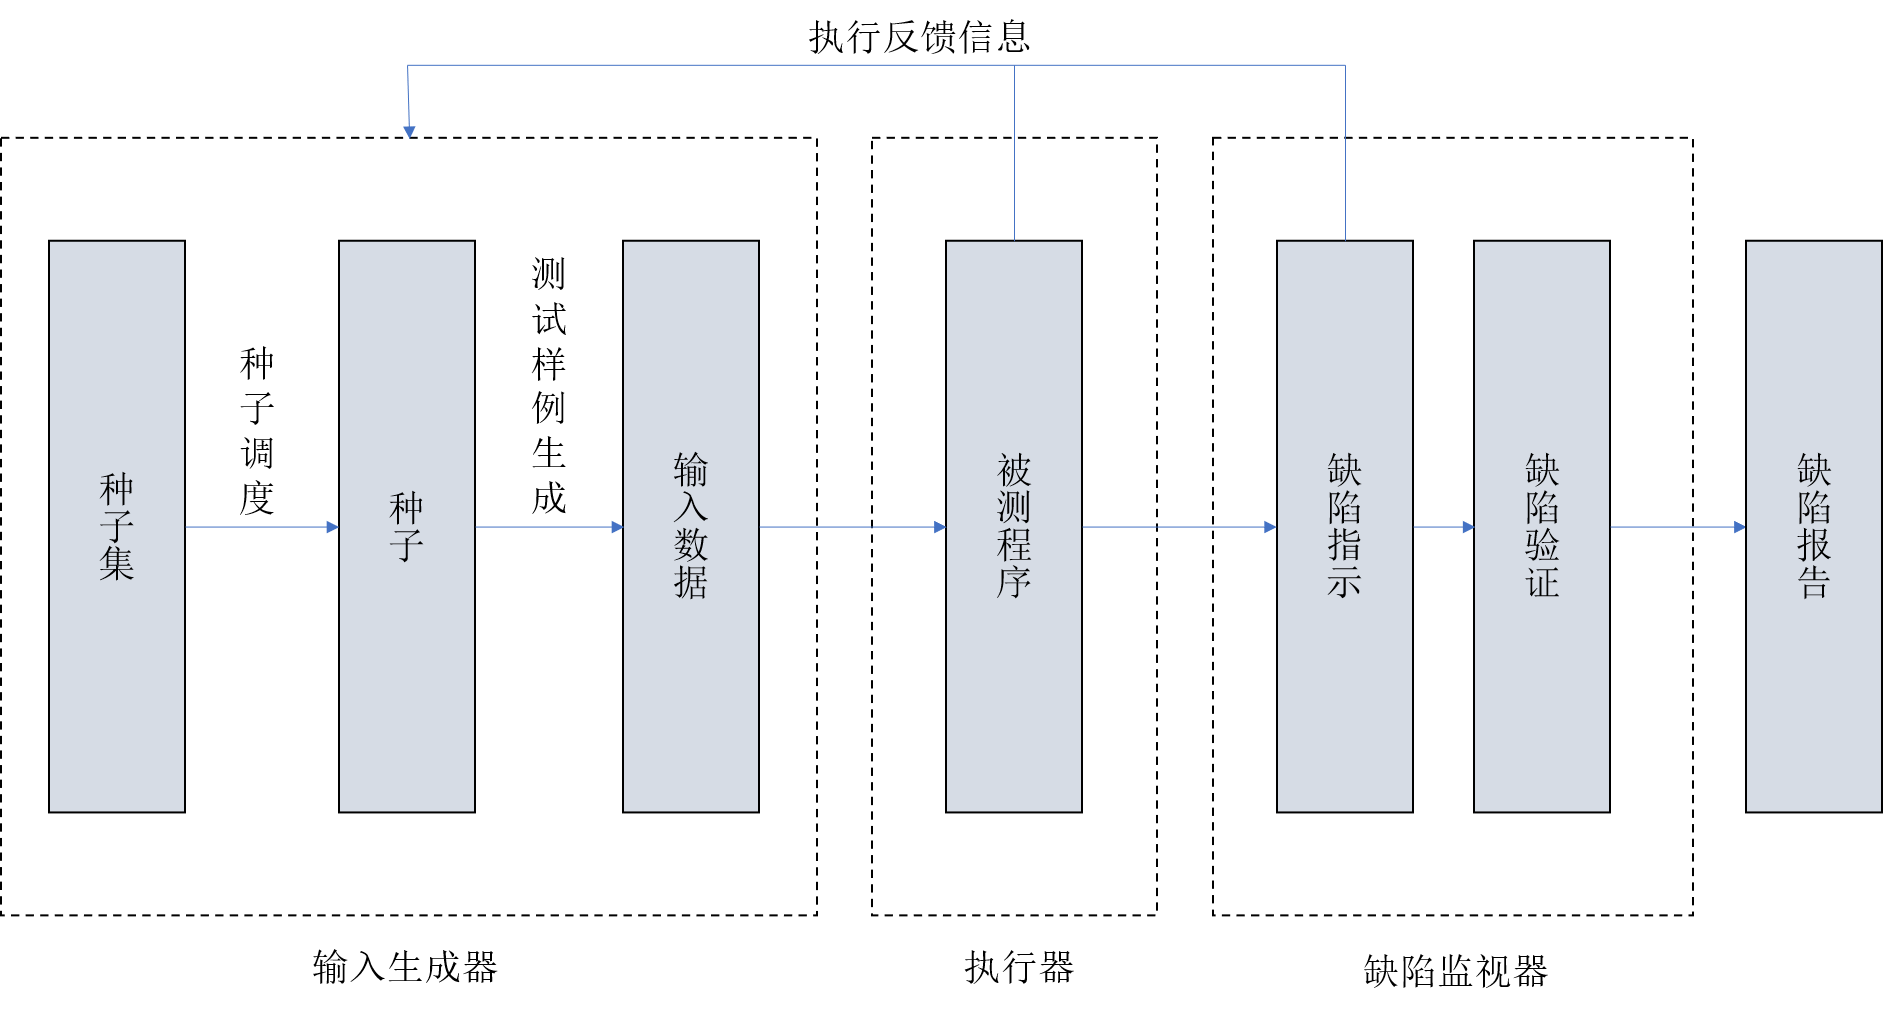
\includegraphics[width=13cm]{fuzzing_workflow.png}
    \caption{通用模糊测试工作流}
    \label{fuzzing_workflow}
\end{figure}

首先解释部分模糊测试中的常用名词,以便后续内容的阅读与理解。

种子(Seed)。在模糊测试中,种子是指作为输入的原始数据或样本。种子可以是各种类型的数据,例如二进制文件、文本文件、图像、音频或视频文件等。种子是模糊测试的基础,因为模糊测试的目标是使用不同的变异或扰动技术生成大量的输入,从而探索应用程序或系统的潜在漏洞或异常行为。

插桩(Instrumentation)。在计算机编程领域,插桩是指在程序的源代码、目标代码或二进制代码中插入代码以收集关于程序执行的信息的过程。在模糊测试中,插桩通常被用来收集关于程序执行的信息,如代码覆盖率、路径覆盖率、函数调用次数等。通过在程序中插入一些用于跟踪程序执行的代码,可以帮助测试人员更好地了解程序的行为,发现潜在的漏洞或错误。

变异(Mutation)。在模糊测试中,变异是指对输入数据进行修改,以便生成新的测试用例的过程。变异可以是随机的,也可以是根据某些规则进行的。变异是模糊测试中非常重要的步骤,因为它可以生成各种不同的测试用例,这些测试用例可以帮助发现程序中的各种漏洞和错误。在变异过程中,可以修改测试用例的任何部分。常见的变异方法包括替换、插入、删除、重排和交换等,这些具体的变异方法也被称作变异算子。

Bug。在计算机科学中,Bug是指程序中的错误或缺陷。当程序在设计、编写或维护过程中出现问题时,就会导致程序的错误或不正常的行为,这种错误或缺陷就被称为Bug。在模糊测试中,测试人员的目标是找出程序中的Bug,以便开发人员能够修复它们。由于模糊测试使用随机和不完整的输入来测试程序,因此可以找到许多开发人员可能没有预料到的程序缺陷。这些Bug可能会导致程序崩溃、安全漏洞、性能问题等。

接下来介绍模糊测试部分常用的分类标准:

根据输入数据生成方法的不同,模糊测试可以分为基于生成的模糊测试和基于变异的模糊测试。基于生成的模糊测试是根据语法规则或有效语料库从零开始生成输入。这种方式下生成的测试用例具备一定的格式约束,通常使用测试人员提供的输入规则,解析得到输入格式,再依据格式生成新的测试用例。基于变异的模糊测试对现有的输入按照一定规则进行修改,以获得新的测试用例。该方式几乎不需要了解待测程序所需的输入格式,因此能够减少测试所需的先验知识。

根据测试目标的不同,可以将模糊测试分为定向模糊测试和非定向模糊测试。定向模糊测试是一种基于先验知识的测试方法,它试图生成能让程序运行到指定位置的输入。定向模糊测试在生成测试用例时利用已知的程序行为或结构信息,有针对性地生成测试用例。例如,根据程序源代码、输入文件格式或API接口规范等先验知识,定向模糊测试可以生成特定类型的测试用例,并尝试抵达程序的特定代码段或调用特定的API接口。这种测试方法可以更快地执行到目标程序中的特定位置。非定向模糊测试希望使测试达到尽可能多的代码覆盖率。它通过随机生成或变异测试用例来测试程序。这种测试方法不关心程序的内部结构和行为,只关注测试用例是否能够触发程序中的错误或异常。非定向模糊测试可以自动化地生成大量测试用例,具有较高的测试覆盖率。

根据程序执行过程中观察到信息量的多少,可以将模糊测试分为黑盒、白盒和灰盒模糊测试。黑盒模糊测试对每个执行程序的内部状态没有任何了解。这些模糊测试工具通常通过利用输入格式或不同的输出状态来优化模糊测试过程。由于其不需要预先获取到程序源代码,因此适用范围更加广泛。但是黑盒模糊测试具有较大的随机性与盲目性,造成测试资源的浪费,测试效率不高。白盒模糊测试获得了每次执行的所有内部知识,使其能够系统地探索目标程序的状态空间。其通常利用动态符号执行技术来分析目标程序并约束求解得到能到达新程序状态的测试用例。理论上,白盒模糊测试可以覆盖程序完整的状态空间。然而实际的测试中,约束求解可能需要花费相当长的时间,甚至可能无法得出有效解。灰盒模糊测试在黑盒和白盒模糊测试之间进行了平衡,能使用插桩等技术获得程序执行状态信息,并利用此信息指导测试用例的生成。

本节的最后介绍部分模糊测试中的常用信息:

模糊测试技术中最常用的信息是被测试程序的执行状态。一种常见的执行状态是代码覆盖率的信息(例如,基本块\citing{nagy2019full}或控制流图中的边\citing{afl2015})。使用覆盖率的基本假设是,发现更多的执行状态(例如,新的覆盖率)会增加发现错误的可能性。例如,安全研究人员发现,代码覆盖率增加1\%,就会增加0.92\%的错误发现\citing{CharlieMiller}。因此,覆盖率引导的模糊测试旨在探索更多的代码覆盖率。然而,由于模糊测试的用途多样,执行状态并不限于代码覆盖率。这些状态也可以是面向对象程序的执行合法性\citing{pacheco2007feedback},协议实现的状态机\citing{li2022snpsfuzzer},并发实现的别名覆盖\citing{xu2020krace},深度学习模型的神经元覆盖\citing{pei2017deepxplore},或安卓智能电视的执行日志\citing{aafer2021android}。

程序的崩溃也是模糊测试经常使用的信息,能够作为发现潜在安全漏洞的参考,因为崩溃提供了直接的自动记录\citing{afl2015}。操作系统会自动产生信号,通知程序崩溃。然而,有些程序缺陷并不表现为崩溃。因此,模糊测试工具可能会使用其他缺陷作为指标,如物理安全侵犯\citing{chen2019learning}。但是这些指标只显示了潜在的安全问题,这些问题要通过安全工具或人工来进一步验证,以确认漏洞\citing{gdb,song2019sok}。

\section{模糊测试关键技术}

模糊测试的算法优化希望使模糊测试能够更有效地暴露缺陷,即模糊测试可以在更短的时间预算或更少的测试用例中发现漏洞。模糊测试根据执行阶段的不同,包含了种子集挑选、种子调度、用例生成和漏洞检测等重要环节。针对这些重要环节,现有的模糊测试工具使用各种解决方案对其进行优化,来提高模糊测试的效率。接下来将对优化模糊测试性能的关键技术进行简要的介绍。

\subsection{种子集挑选技术}

%todo
% 由于 AFL 的流行,afl-cmin [40] 可能是使用最广泛的语料库蒸馏工具。它实现了贪心蒸馏算法,但具有独特的覆盖方法。特别是,afl-cmin 重用 AFL 自己的边缘覆盖概念在蒸馏时对种子进行分类,记录边缘频率计数的近似值,而不仅仅是边缘是否已被占用。蒸馏时,afl-cmin 选择集合语料库中覆盖给定边的最小种子,然后进行贪心加权蒸馏。

种子集挑选技术的目标是最小化种子集,即选择能够覆盖所有发现的代码覆盖率的最少数量的种子\citing{afl2015}。最小化的原因是,无论是测试提供的初始种子,还是模糊测试过程中新加入的种子,它们之间都可能存在冗余信息,从而浪费了检查已探索过的代码区域的计算资源。最小化种子集的问题本质上为最小集覆盖问题,它最小化包含所有元素的子集。由于最小集覆盖问题是一个NP-hard问题,许多研究者采取贪心算法来解决该问题。afl-cmin 重用 AFL 的边缘覆盖概念,在精简时对种子进行分类,记录边缘频率计数的近似值,选择集合语料库中覆盖给定边的最小种子,然后进行贪心加权精简。COVERSET\citing{rebert2014optimizing}使用一个贪心多项式近似算法来获得最小集。

\subsection{种子调度技术}

确定种子集后,种子调度旨在解决以下问题:1)下一轮要选择哪颗种子;2)所选种子的时间预算。在实际工程实现上,大多数模糊测试工具并不对时间预算进行优化,而是对选定种子的变异次数进行优化\citing{yue2020ecofuzz}。虽然这两个问题相当明确,但由于测试环境或漏洞的复杂性,现有的优化解决方案也各不相同。最关键的挑战是对未发现的代码覆盖或漏洞的未知。在验证漏洞之前,测试人员无法预知一个输入是否能触发漏洞;因此,种子调度的优化问题没有一个有效的适配性。类似未知的还有,在检查源代码之前,测试人员无法获得程序行为(例如,分支行为)的概率分布;因此不可能从数学上找到全局最优解。由于上述挑战,研究人员根据不同的优化问题大致或部分地制定了模糊测试过程。

通常,模糊测试利用两种类型的优化问题适应度,即基于漏洞或执行状态(例如,代码覆盖率)的适应度。适应度是衡量种子或输入质量的标量。对于基于漏洞的适应度,研究者会对待测试程序进行预处理,标记出可能存在漏洞的危险代码段,计算得到当前种子对应的执行路径与危险代码段的距离,距离越短意味着由该种子生成的测试用例更有可能使程序执行到危险代码段\citing{chen2020savior}。由于模糊测试将专注于与发现的错误相关的代码区域。因此它可能会错过探索更多代码覆盖率的机会。在这种情况下,受复杂条件保护的深层错误可以逃避模糊测试。为了缓解这个问题,许多模糊测试工具根据执行状态计算适应度,因为执行状态可以为模糊测试提供更多信息。大多数现有的模糊测试工具根据代码覆盖率计算适应度;也就是说,他们以提高代码覆盖率作为研究目标。使用代码覆盖率作为指标还有另一个原因,即更大的代码覆盖率表明发现错误的可能性更高。

\subsection{用例生成技术}

如前所述,模糊测试中的测试用例是通过基于生成的方法或基于变异的方法产生的。

在基于生成的模糊测试中,生成器根据对输入数据格式的了解,生成测试用例。许多常用的文件格式都提供了文档,模糊测试工具可以根据文档中的格式信息生成测试用例。但部分的文件格式并未公开,如何获得处理这类文件的软件输入格式信息是一个很难解决的问题。机器学习技术和形式化方法能够被用来解决这个问题。文献\cite{godefroid2017learn}使用机器学习技术,特别是递归神经网络,来学习输入文件的语法,并使用学到的语法来生成满足格式的测试案例。文献\cite{wang2017skyfire}使用格式化的方法,具体而言,它定义了一个概率上下文敏感的语法,并提取格式知识,以生成格式良好的种子输入。

更多最先进的模糊测试工具\citing{lemieux2018fairfuzz,lyu2019mopt,chen2018angora}采用基于变异的模糊测试策略。它们通过修改变异过程中的部分种子输入来生成测试用例。在盲目变异模糊测试过程中,变异器随机修改种子字节为随机值或几个特殊值,这被证明是非常低效的。因此如何确定修改的位置和修改时使用的值是另一个关键挑战。在基于覆盖的模糊测试中,应首先修改可能影响控制流传输的字节。污点分析技术用于跟踪字节对控制流的影响,以定位变异种子的关键字节,这些关键字节将成为变异的重点位置\citing{rawat2017vuzzer,chen2018angora}。由于污点分析会带来额外的时间开销,因此部分工作仍使用启发式算法来选择变异算子和变异的位置\citing{wu2022one, zhang2022path}。

\subsection{漏洞检测技术}

许多安全漏洞可以被利用来控制系统,泄露私人数据,或破坏服务器\citing{cwe25}。检测漏洞的挑战在于,漏洞是不可预测的。具体来说,漏洞检测工具不知道错误的位置,甚至在测试之前不知道目标程序中是否存在漏洞。因此,在模糊测试过程中自动记录一个潜在的漏洞是非常关键的。通常情况下,指标是程序执行的崩溃,但还有一些指标是基于漏洞模式设计的。虽然漏洞模式只能用来暴露特定类型的漏洞,但如果目标程序中存在这种类型的漏洞,它就非常有效。本小节将介绍六种通过模糊测试技术成功检测到的漏洞。它们是内存违反漏洞(Memory-violation Bugs)、并发漏洞(Concurrency Bugs)、算法复杂性漏洞(Algorithm Complexity Vulnerability)、幽灵型漏洞(Spectre-type Bugs)、侧信道漏洞(Side-channel Bugs)和整数溢出漏洞(Integer Overflow Bugs)。

(1)内存违反漏洞

\begin{figure}[!htbp]
    \vspace{6pt}
    \subfloat[]{
        \label{MemoryBugA}
        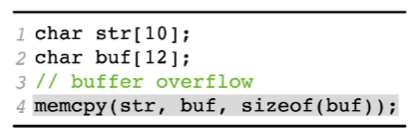
\includegraphics[width=6cm]{MemoryBugA.png}
    }
    \subfloat[]{
        \label{MemoryBugB}
        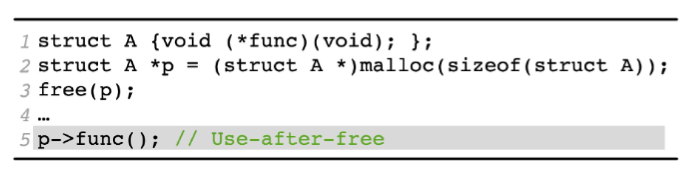
\includegraphics[width=9cm]{MemoryBugB.png}
    }
    \caption{内存违反漏洞(a)空间安全违反;(b)时间安全违反}
    \label{MemoryBug}
\end{figure}

%todo [131、175、178] [175]
内存安全违反是最古老和最严重的安全错误之一。如果指针仅限于访问预期的引用对象,则程序是内存安全的。内存安全违反可分为两类,即空间安全违反和时间安全违反。空间安全违反会访问越界的内存,而时间安全违反会访问无效的引用对象。例如,图\ref{MemoryBugA}是空间违规,因为 buf 的大小大于 str(缓冲区溢出)。另一方面,图\ref{MemoryBugB}是时间违规,因为指针 p 在释放后被再次使用。尽管已经提出了许多方法来减轻内存安全违反的影响,但由于性能开销、兼容性低和鲁棒性低等缺点,大多数方法都没有在实践中使用。

部分非法内存访问会因为操作系统的内存保护机制而发送特殊信号给程序,使得程序直接崩溃。但是部分非法内存访问并不会被程序直接识别出来,程序会继续往下执行。为了解决这个问题,模糊测试通常引入内存消毒剂技术\citing{asan},使得程序在发生非法内存访问时主动中止并记录异常,从而发现正常程序运行无法发现的漏洞。

(2)并发漏洞

并发漏洞也是一种常见且可能导致严重危害的漏洞,当并发程序在没有正确同步或顺序的情况下运行时会发生这种错误。常见的并发漏洞包括:1)竞争条件漏洞。在多线程环境下,两个或多个线程同时访问同一个资源,并且它们之间的执行顺序不确定。如果程序没有正确处理这些竞争条件,可能会导致不一致的状态或者不安全的操作。2)死锁漏洞。在多线程环境下,两个或多个线程同时等待对方释放锁,从而导致程序陷入死锁状态。3)非原子操作漏洞。在多线程环境下,某些操作需要多个步骤才能完成,如果这些步骤没有被原子化,就可能导致竞争条件问题。4)内存共享漏洞。在多进程或分布式环境下,多个进程或节点共享同一块内存区域,如果没有正确处理共享内存的访问,就会导致安全漏洞。

并发漏洞的发生是由于线程不正确地交错执行指令。发现该漏洞的困难在于并发程序可能有太多的交错,无法逐一检查(即状态爆炸问题)。基于一些交错是等价的这个事实可以缓解状态爆炸问题,因为它们来自非交互指令的不同执行顺序。这种等价性表明,它们的执行将导致相同的状态。如模糊测试工具CalFuzzer\citing{Calfuzzer},它随机选择一组线程,这些线程的后续指令互不交互,并同时执行这些指令。因此,CalFuzzer可以更有效地检查不同的交织方式。

(3)算法复杂性漏洞

当算法在最坏情况下的复杂性显著降低性能时,就会出现算法复杂性漏洞,这可能会导致拒绝服务 (Denial of Service,DoS) 攻击。以快速排序算法为例,待排序数组的数据分布会使得算法具有不同的时间复杂度。其平均时间复杂度为$O(nlogn)$,然而最坏时间复杂度达到了$O(n^2)$,当输入的特定的数据时,快速排序算法的性能会显著下降。因此,最坏情况下的行为可能会被攻击者利用来发起 DoS 攻击。

为了发现算法复杂度漏洞,可以将执行指令数量和内存消耗当作反馈的指标,执行指令多说明程序可能存在潜在的算法时间复杂度漏洞,内存消耗多说明程序可能存在潜在的空间算法复杂度漏洞。如模糊测试工具SlowFuzz\citing{petsios2017slowfuzz} 通过将模糊测试引导到增加执行指令数量的路径来检测算法复杂度漏洞;模糊测试工具MemLock\citing{wen2020memlock}基于边缘覆盖和内存消耗这两个指标来检测算法复杂度漏洞,它将模糊测试引向可以发现更多边缘覆盖或消耗更多内存的输入。

(4)幽灵型漏洞

%todo
幽灵型漏洞是一种微体系结构攻击,它的出现是因为CPU设计的分支预测机制,该机制可以预测下一条指令的分支是跳转还是继续执行,从而提高指令的执行效率。攻击者可以利用这个机制,通过构造恶意代码来迫使CPU预测错误,从而访问不属于它的内存数据\citing{oleksenko2020specfuzz}。模糊测试工具SpecFuzz\citing{oleksenko2020specfuzz} 检测目标程序来模拟推测执行,这可以强制执行错误预测的代码路径。然后可以触发错误预测路径中的非法内存访问。

% 例如,在图 10 中,攻击者可以为变量输入发送多个边界内的值,这将训练分支预测器推测第 2 行中的检查是否始终为真。当攻击者为输入发送越界值时,预测器将错误地预测分支行为,并且推测性地执行第 3-4 行(即,它们在第 2 行中没有检查的情况下执行)。由于输入实际上不满足第 2 行的检查,因此第 3-4 行的执行导致缓冲区溢出。因此,

(5)侧信道漏洞

侧信道漏洞通过观察系统的非功能行为(如执行时间)来泄露秘密信息。例如,如果一个秘密是语句 "if (a > 0){...}else{...}"中的变量a,人们可以观察then-branch和else-branch的执行时间来判断a的值是否大于0。一种特殊的侧信道被称为JIT诱导的侧信道,它是由即时(Just-In-Time,JIT)优化引起的\citing{brennan2020jvm}。与前面提到的幽灵型漏洞类似,人们可以反复运行程序来训练JIT编译器优化then-branch或else-branch的执行时间。然后,训练过的分支(如then-branch)和未训练过的分支(如else-branch)的执行时间将有足够的偏差以供观察,进而推测得出变量a的秘密值。

(6)整数溢出漏洞

整数溢出漏洞是指在计算机程序中,对于某些整型变量,当其存储的数值超出了该整型变量的表示范围时,会发生溢出,导致程序出现意外行为。通常情况下,当整型变量的数值超出了其表示范围,会发生截断,即将其截断为其能够表示的最大或最小值。然而,在某些情况下,由于程序设计不当或者缺乏对整数溢出的检测,可能会导致程序出现未预期的行为,从而成为整数溢出漏洞。为了去检测整数溢出漏洞,模糊测试工具SmartFuzz\citing{molnar2009dynamic} 根据不同的整数错误将特定约束添加到符号仿真中。然后,符号求解器将生成可能触发整数错误的具体输入。

\section{模糊测试评价指标}
为了客观评估模糊测试工具的测试能力,需要使用通用的评价指标对测试结果进行评估。常用的模糊测试评价指标包括发现的崩溃数和代码覆盖率。

\subsection{崩溃数}

发现软件漏洞是模糊测试的最终目标,但直接发现漏洞是相当困难的,因此大多数模糊测试工具把程序的崩溃视为一个潜在的漏洞。程序崩溃意味着当前的输入会导致程序处理出错而意外退出,这表明程序中的潜在漏洞可能已经被触发。可以通过当前测试用例下待测程序是否接收到操作系统发出的致命信号(例如SIGKILL、SIGSEGV等)来判断程序是否发生崩溃。判断崩溃是否重复的方法是比较导致程序崩溃的执行路径是否相同,如果相同,则认为这两个测试用例触发了相同的崩溃。

然而执行路径的不同并不一定代表发现了不同的漏洞,大多数漏洞的成因与堆栈中最接近顶部的部分最为相关。在这种情况下,可以查看调用堆栈,将最近的N个堆栈帧与某个特定错误的触发联系起来(N通常被选为3到5之间)。这些堆栈信息可以被哈希化,以便与之前的错误进行快速比较\citing{klees2018evaluating}。

%todo asan图片

\subsection{代码覆盖率}

模糊测试是为了寻找程序中的漏洞。如果一个模糊测试工具运行了很长时间却没有发现任何错误,那么它的用户会认为它是不成功的。根据模糊测试工具发现的错误数量来评估模糊测试工具似乎是合乎逻辑的。然而,仅仅因为模糊测试工具没有找到漏洞,可能并不能告诉测试人员关于模糊测试工具效率的全部情况。也许它的算法是正确的,但由于被测试程序本身漏洞很少或不存在漏洞,模糊测试工具并不一定能发现漏洞。

之前对测试套件有效性的研究表明,代码覆盖率与发现漏洞的有效性存在正相关\citing{gopinath2014code}。因此代码覆盖率成为了评价模糊测试工具性能的另一个有效指标。

典型衡量代码覆盖率的指标有:行覆盖、分支覆盖、路径覆盖\citing{cov}。

(1)行覆盖

行覆盖是指在软件测试中,测试用例执行后能够覆盖到代码中的每一行。如果一行代码被测试用例执行到了,那么该行就被认为是被覆盖的。

(2)分支覆盖

分支覆盖是指在软件测试中,测试用例执行后能够覆盖到代码中的每一个分支语句。分支语句指的是if、else、switch、case等分支结构。如果一个分支语句被测试用例覆盖到了,那么该分支就被认为是被覆盖的。

(3)路径覆盖

路径覆盖是指在软件测试中,测试用例执行后能够覆盖到代码中的每一条路径。路径指的是程序执行的路径,即从程序的入口到出口所经过的所有语句序列。路径覆盖的目标是使得程序中所有的路径至少被测试用例中的一个执行过程覆盖一次。

\section{本章小结}

本章首先介绍了模糊测试的概念和通用的测试流程。然后介绍了模糊测试常见的一些分类标准和模糊测试中常用的信息。接下来重点介绍了模糊测试中的关键技术,包括种子集挑选、种子调度、用例生成、漏洞检测等技术。最后介绍了两种典型的模糊测试评价指标,包括崩溃数和代码覆盖率。

\chapter{动态策略并行模糊测试系统方案设计}

本章首先介绍并行模糊测试的基础模型,然后分析现有方案的优点以及存在的不足,进而针对这些不足提出本文并行模糊测试的研究目标,最后针对研究目标设计动态策略并行模糊测试系统。

\section{并行模糊测试基础模型}
本节将介绍一个描述并行模糊测试的模型\citing{wang2021facilitating}。该模型包含现有模糊测试工具中的并行模式,它的通用性足以应用于其他并行模糊测试解决方案。

形式化来说,并行模糊测试系统由$n$个模糊测试实例$\{F_1, F_2, ..., F_n \}$组成。这些实例共同处理一组$m$个任务$\{T_1, T_2, ..., T_m \}$。其中,第$i$个实例被分配以专注执行任务子集$\{T_{i1}, T_{i2}, ..., T_{im_i}\}(m_i \leq m)$。根据任务的定义,$\{T_1, T_2, ..., T_m \}$可能需要完成不同数量的工作量$\{W_1, W_2, ..., W_m \}$。为了提高并行模糊测试的效率,并行模糊测试系统需要满足以下三个属性。

\textbf{不同的实例应该处理不相交的任务子集。}这是为了避免重叠并增加并发程度。形式上,给定任意两个实例$F_i$和 $F_j (i \neq j)$,模糊测试系统需要确保:
\begin{equation}
\{T_{i1}, T_{i2}, ..., T_{im_i}\} \bigcap \{T_{j1}, T_{j2}, ..., T_{jm_j}\} = \emptyset
\label{eq1}
\end{equation}

\textbf{所有的实例加起来应该涵盖所有的任务。}形式化上看,这意味着:
\begin{equation}
\bigcup_{i = 1}^{n} \{T_{i1}, T_{i2}, ..., T_{im_i}\} = \{T_{1}, T_{2}, ..., T_{m}\}
\end{equation}

否则,并行模糊测试可能会导致某些任务丢失,从而可能会错过那些任务可以覆盖的代码。

\textbf{不同的任务应被分配类似的工作量。}形式化上看,模糊测试系统应该在任何两个实例之间保持以下关系:
\begin{equation}
\sum_{n = 1}^{m_i}W_{in} \approx \sum_{n = 1}^{m_j}W_{jn} 
\end{equation}

否则,某些实例可能会收到负载不足的任务,并以大量的空闲周期结束,这在原则上也会损害并发性。

虽然上述模型很普遍,但它忽略了一个事实,即同一个任务被不同的模糊测试实例执行可能带来不同的收益,特别是在代码覆盖率上的提升\citing{chen2019enfuzz}。具体来说,同一个任务,分发给运行不同模糊测试算法的实例进行测试,由于其变异算法、评估算法等的不同,得到的最终效果会存在差异性,测试结果可能存在互补的情况。因此,对于同一测试任务,给它分配到唯一的模糊测试实例进行测试,并不一定达到最优的测试效果。

综上,方程\ref{eq1}应该被修正,以允许具有较高收益的任务重叠,这样这些任务就有较高的机会被选中并被不同的模糊测试实例执行。为了纳入这一考虑,并不是必须修改提出的模型。相反,可以复制高回报的任务,并把它们的复制体视为独特的任务。这将达到与允许这些任务重叠的类似效果。

\section{现有方案分析}

目前,并行模糊测试技术主要是采用同构的方式,也有一些并行模糊测试工具采用了异构的设计。如图\ref{classify}所示,常见的同构并行模糊测试工具有AFL、Pafl、Ultrafuzz等,其中AFL工具应用最为广泛;异构并行模糊测试工具有EnFuzz与Collabfuzz。下面将介绍业界广泛使用的并行模糊测试工具AFL和近年来在同构方向研究中最为出色的并行模糊测试工具Ultrafuzz、异构方向方向研究中最为出色的并行模糊测试工具Collabfuzz。

\begin{figure}[!htbp]
    \vspace{6pt}
    \centering
    
\includegraphics[width=13cm]{classify.png}
    \caption{并行模糊测试工具分类}
    \label{classify}
\end{figure}

(1)AFL

AFL 支持并行模糊测试以完全利用多核机器上的可用资源并加快模糊测试过程。在这种情况下,每个 AFL 实例独立执行,它们之间没有明确的资源竞争关系。从 AFL 设计的角度来看,模糊测试操作应该随着核心数量的增加而线性扩展。此外,为了避免对文件系统访问的明显争用,每个 AFL 实例都在其用于测试用例的私有工作目录中工作。在模糊测试循环结束时,AFL 实例扫描其他实例的输出目录以了解它们的测试用例,称为同步阶段。对于每个协作邻居,它保留一个测试用例标识符,指示它检查的最后一个测试用例。它找出所有标识符大于保留标识符的测试用例,并逐个重新执行它们。如果测试用例覆盖了实例本身尚未发现的新路径,则测试用例将被复制到它自己的目录中以进行进一步的变异。图\ref{aflp}展示了AFL并行模糊下的架构。

\begin{figure}[!htbp]
    \vspace{6pt}
    \centering
    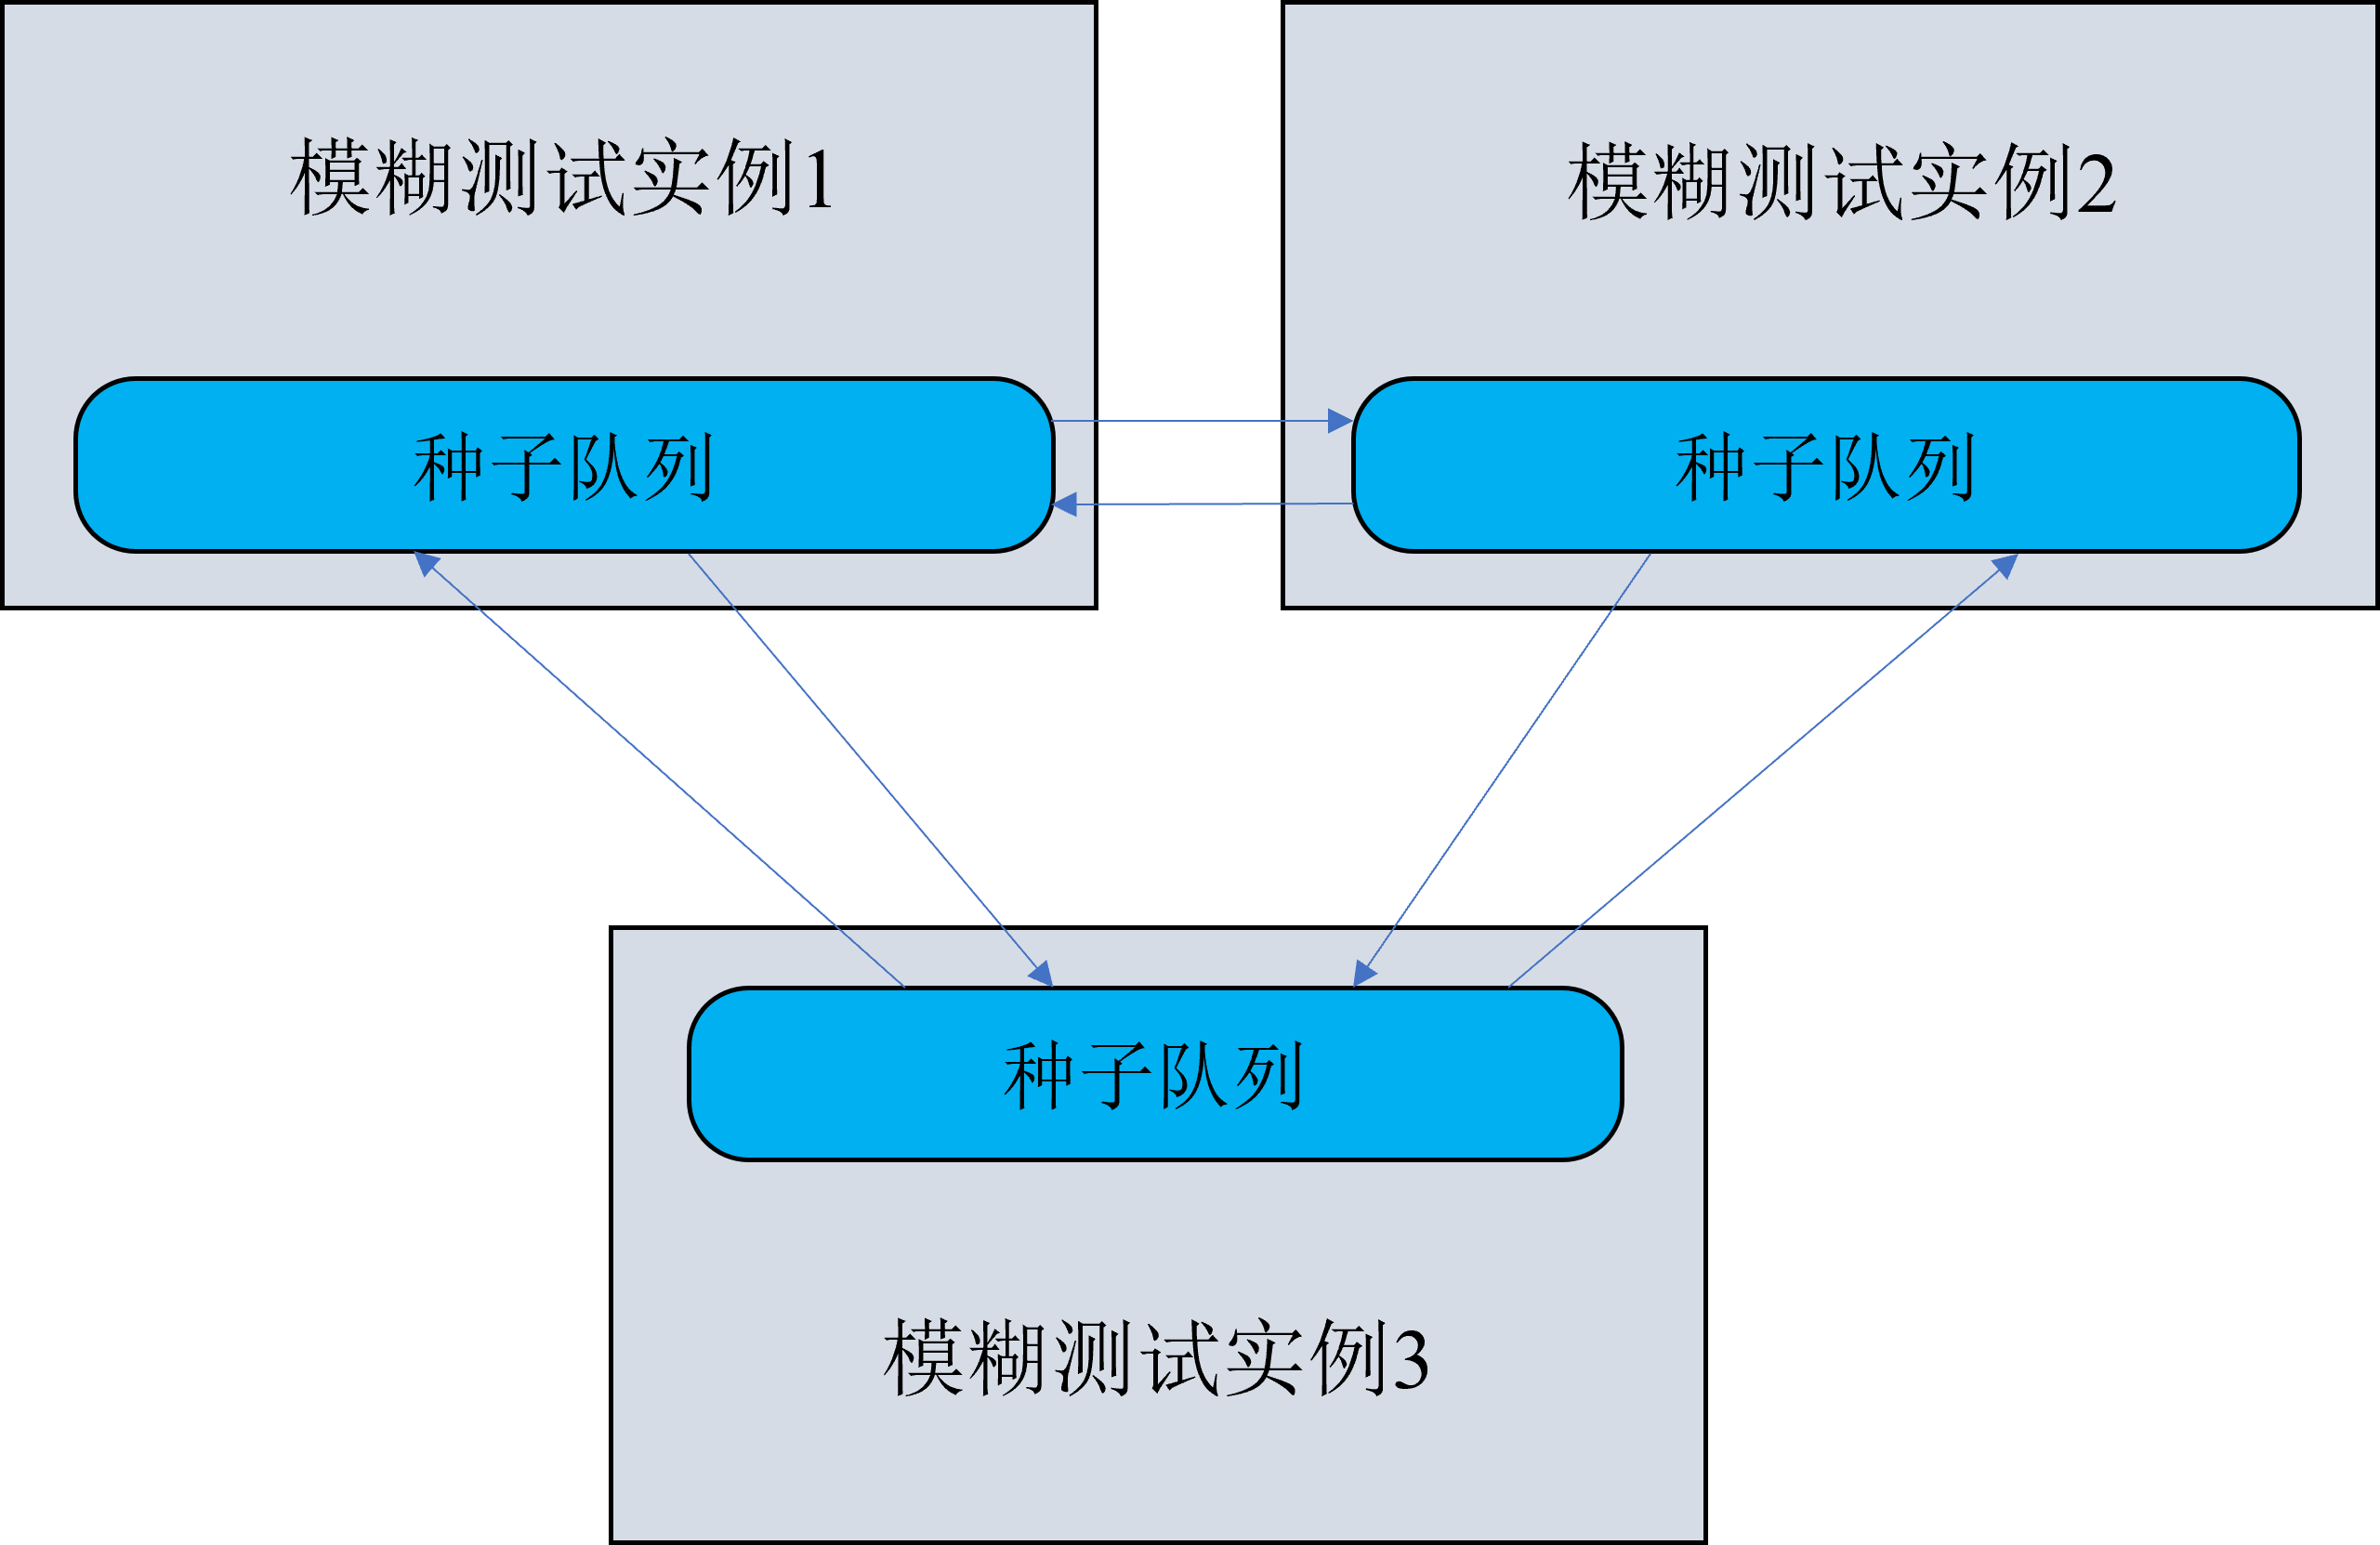
\includegraphics[width=11cm]{afl-p.png}
    \caption{AFL并行模式架构}
    \label{aflp}
\end{figure}

AFL工具的并行模式实现简单,各个模糊测试实例较为独立,使得整个系统鲁棒性强,即使一个节点失效,也不会影响其他节点的测试。但是这样的特性也有其缺点,各实例之间信息交流极少,使得测试可能存在大量冗余,浪费了宝贵的系统资源。

(2)Ultrafuzz

%todo arrow

\begin{figure}[!htbp]
    \vspace{6pt}
    \centering
    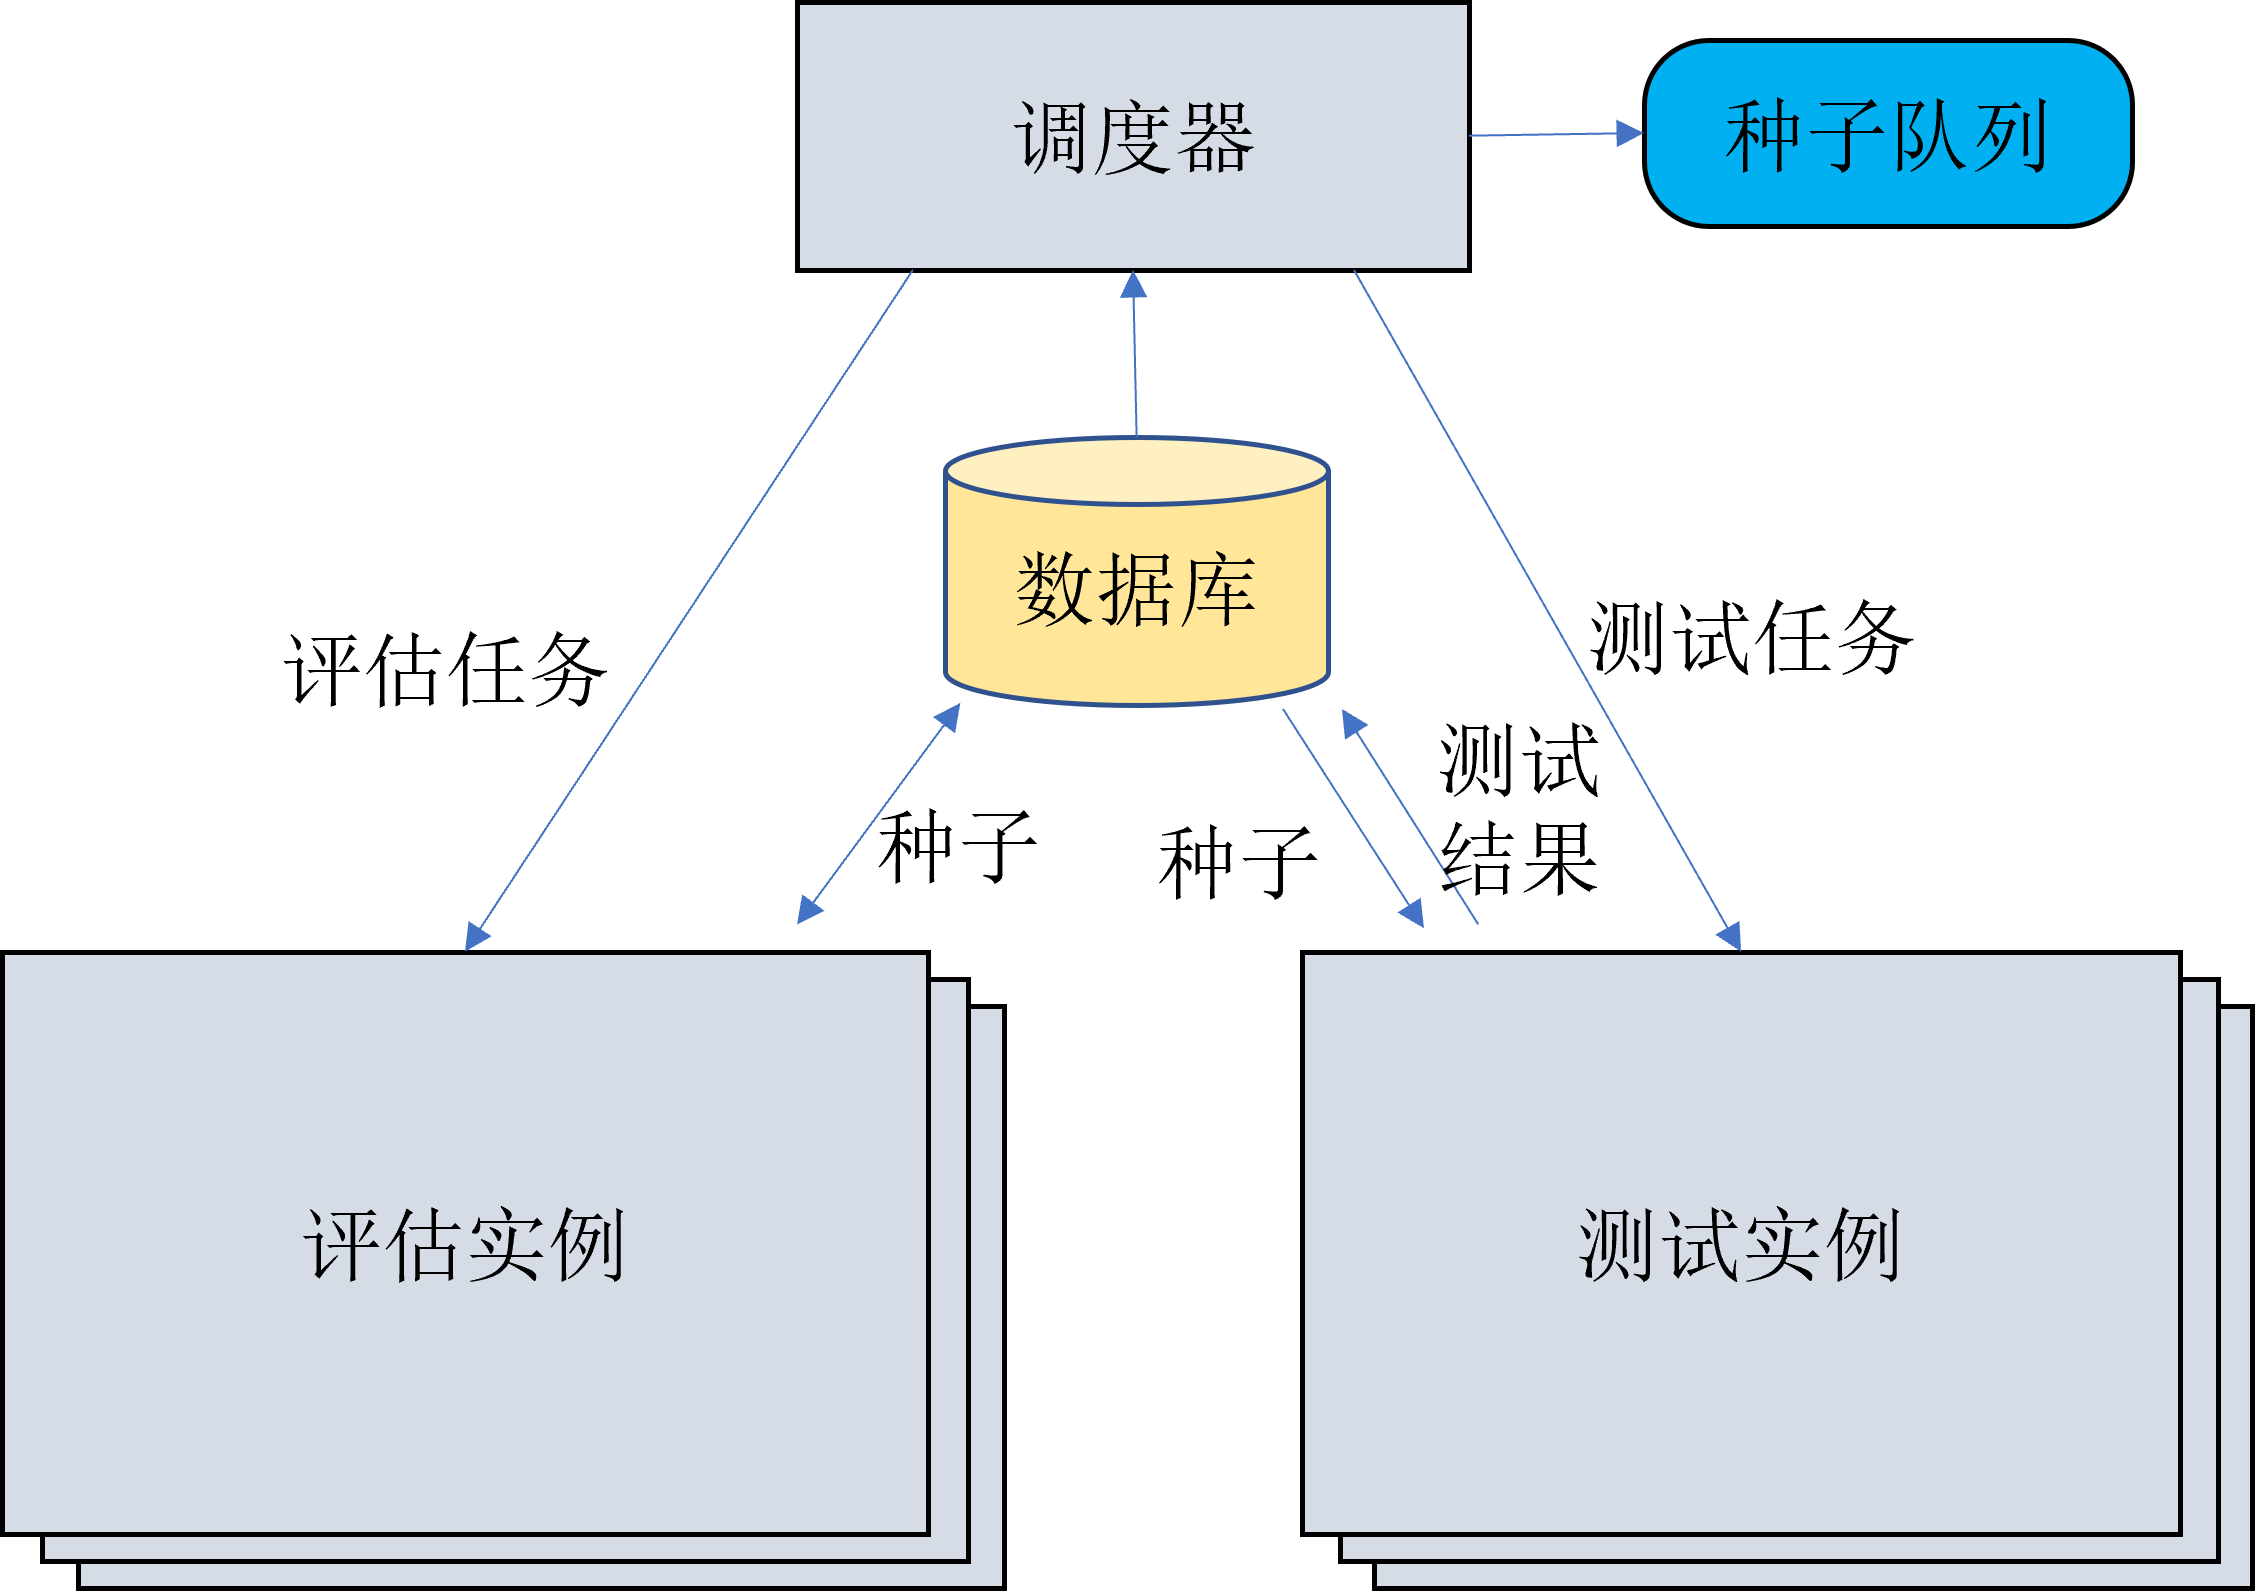
\includegraphics[width=10cm]{ultrafuzz.png}
    \caption{Ultrafuzz架构图}
    \label{ultrafuzz}
\end{figure}

Ultrafuzz使用集中式动态调度,从种子选择、能量调度、模糊状态同步和任务调度等方面全面优化分布式模糊测试。如图\ref{ultrafuzz}所示,模糊测试架构由四个部分组成:一个调度器、一个数据库、模糊测试实例和评估实例。在组成分布式系统的计算节点中,选择一个作为主节点,其余的为工作节点。工作节点用于进行测试执行或评估种子。

在主节点上,Ultrafuzz设计了一个调度程序来调度种子评估、对队列中的种子进行优先排序、处理来自模糊测试实例的请求以及调度模糊测试任务。模糊测试任务包含两种信息:种子的索引(即哈希值)和指示种子应变异多少次的整数(即能量)。同时,在主节点上部署了一个数据库,用于存储和共享模糊测试数据(例如,种子、模糊测试状态和覆盖率)。每个模糊测试实例都连接到数据库以同步模糊测试信息和种子。

对于工作节点,它既可以作为模糊测试实例,也可以作为评估实例。模糊测试实例负责运行测试用例和变异种子。它从数据库中下载调度程序分配的任务种子,并将新的种子上传到数据库中。大多数计算核心用于运行模糊测试实例。评估实例用于过滤掉重复的种子,使得模糊测试实例可以下载唯一的种子。

这种集中式动态调度将调度与模糊测试分开,可以从全局角度选择种子和调度功率,缓解任务冲突造成的资源浪费问题,将机器内的并行模糊测试扩展到分布式环境中的机器之间。但是这种架构仍然存在一定的局限性,它只能使用一种调度策略和测试用例生成策略,如果这些策略本身对被测试程序效果不佳,并行后的模糊测试效果也有限。

(3)Collabfuzz

\begin{figure}[!htbp]
    \vspace{6pt}
    \centering
    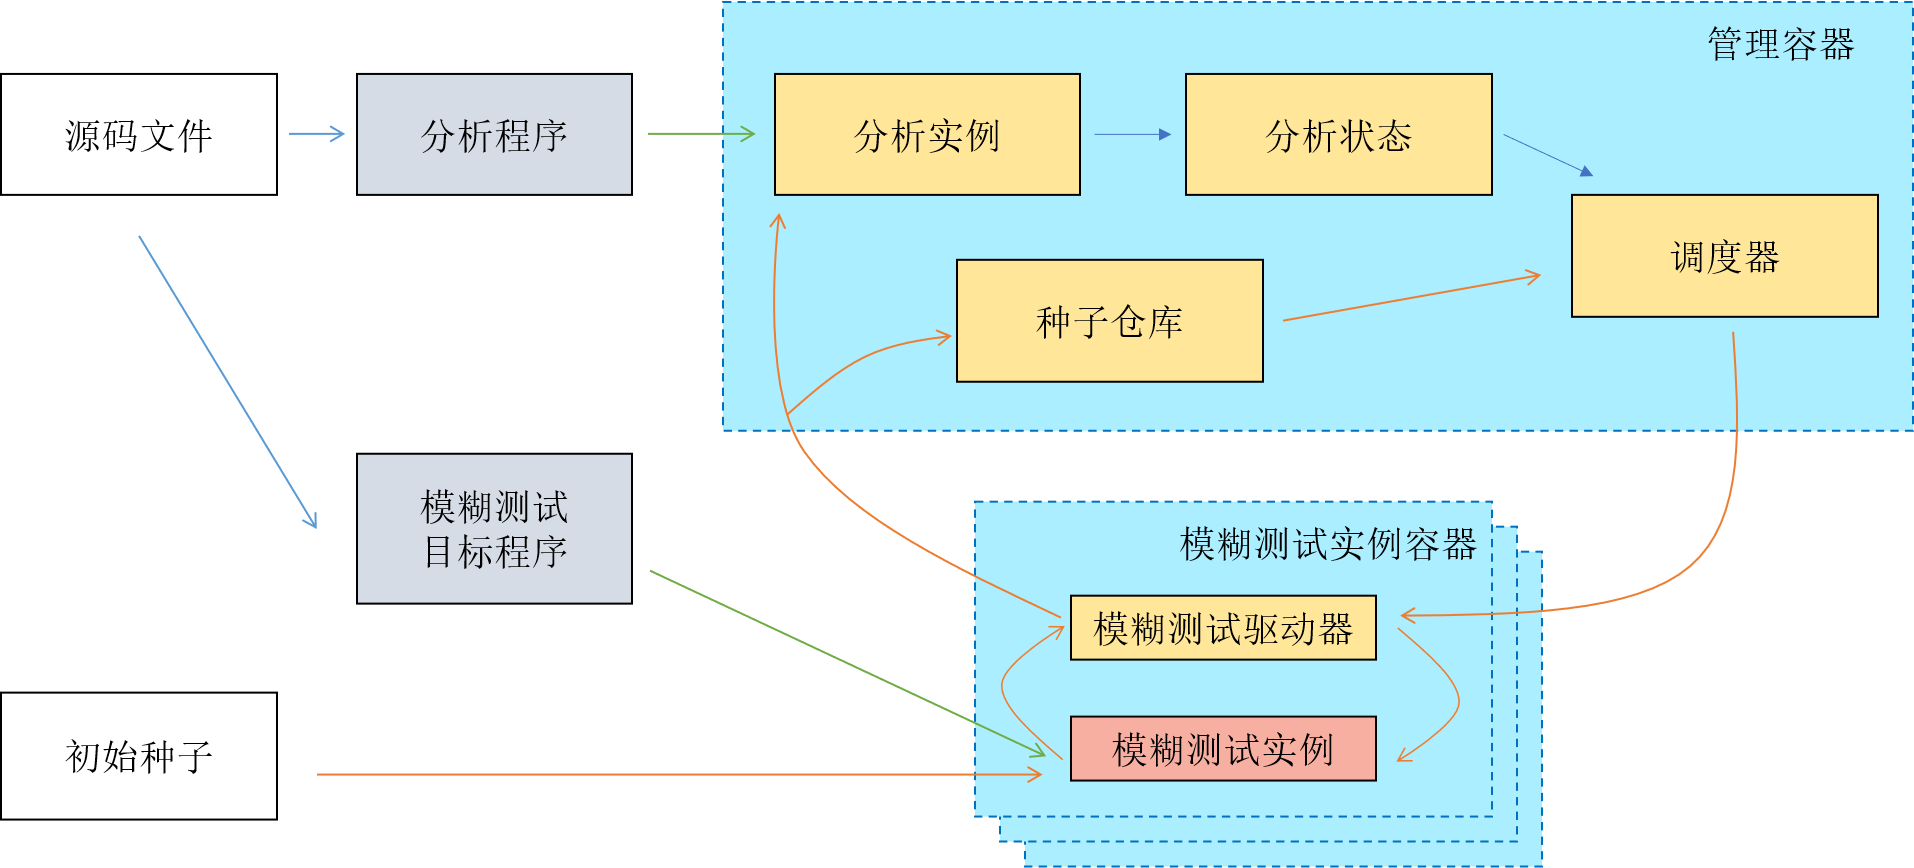
\includegraphics[width=15cm]{collabfuzz.png}
    \caption{Collabfuzz架构图}
    \label{collabfuzz}
\end{figure}

Collabfuzz是一个协作模糊测试框架,允许多个不同的模糊测试工具在基于大量中央分析的知情调度策略下进行协作。更具体地说,Collabfuzz 是一个通用框架,允许用户表达不同的测试用例调度策略,例如 EnFuzz 提出的协作方法。 Collabfuzz 可以控制将哪些测试用例分发给哪个模糊测试实例,并允许跨网络编排不同的模糊测试实例。此外,它允许集中分析其控制下的各种模糊测试实例生成的测试用例,允许根据任意程序(例如数据流)分析的结果实施调度策略。

对于一次运行,Collabfuzz必须提供被测程序的源代码、该程序的一组种子、要运行的模糊测试工具组合以及协调它们的策略。如图\ref{collabfuzz}所示,源程序将被编译成几个工具化的二进制文件(将用于分析测试案例)和每个模糊测试工具所需的所有二进制文件。之后,该框架可以被启动。在运行过程中,以下三个组件值得关注:

(1)中央管理器。该组件根据用户设置的调度策略将测试用例调度到不同的模糊测试实例。

(2)模糊测试实例。用户可以将任何现成的模糊测试工具添加到组合中。这些模糊测试实例获取测试用例并对其进行变异,通常会针对寻找新的覆盖范围进行优化。 

(3)模糊测试驱动器。驱动程序与现成的模糊测试实例交互,在中央管理器需要安排它们时将新的测试用例交给它,并将新发现报告给中央管理器。

在收到来自一个驱动器的新测试用例时,管理器首先将收到的测试用例放入存储空间,然后它启动许多由调度程序定义的分析实例。例如,调度程序可能需要覆盖率分析,在这种情况下,管理器将在分析实例上为传入的测试用例启动覆盖率收集工作。这些分析实例的结果存储为分析状态,稍后调度程序可以在做出调度决策时查询这些状态。

当新的测试用例到达管理器时,调度程序会定期(以用户可配置的时间间隔)和以事件驱动的方式被调用,从而在实施调度策略时提供最大的灵活性。当调用调度程序时,它可以对存储的分析状态进行推理,然后就是否将零个或多个测试用例分发给任何正在运行的模糊测试实例做出决定。当调度程序做出决定时,选定的测试用例将发送到相应的模糊测试实例驱动器。然后将新的测试用例插入到模糊测试实例的种子队列中。

Collabfuzz提供了对不同模糊测试工具较为通用的支持,相比于并行化后模糊测试算法固定的同构并行模糊测试,不同模糊测试工具共享信息并行化地进行模糊测试有一个显著的优点。图\ref{motivation}是该优点的简易示例\citing{chen2019enfuzz}。

该示例将两个字符串作为输入,并在两个字符串之一为“Magic Str”,而另一个字符串为“Magic Num”时崩溃。许多现有的模糊测试策略往往是根据某些偏好设计的。假设有两个不同的模糊测试工具 fuzzer1 和 fuzzer2,fuzzer1 擅长解决“Magic Str”问题,因此它更好地达到目标 T1 和 T3,但未能达到目标 T2 和 T4。fuzzer2 擅长解决“Magic Num”问题,因此可以更好地达到目标 T2 和 T6,但未能达到目标 T1 和 T5。如果分别使用这两个模糊测试工具进行测试,测试只能覆盖一条路径和两个分支。如果同时使用它们并在没有种子同步的情况下集成它们的最终模糊测试结果,可以覆盖两条路径和四个分支。然而,如果在整个模糊测试过程中将这两个模糊测试工具与一些同步机制结合在一起,那么,一旦 fuzzer1 达到 T1,它就会同步可以覆盖 T1 到 fuzzer2 的种子。在这个同步种子的帮助下,fuzzer2 也可以达到 T1,并且由于它能够解决“Magic Num”问题,fuzzer2 可以进一步达到 T4。同样,借助fuzzer2同步的种子输入,fuzzer1也可以进一步到达T2和T5。因此,通过这种集成方法可以涵盖所有四个路径和所有六个分支。

\begin{figure}[!htbp]
    \vspace{6pt}
    \subfloat[]{
        \label{crash_code}
        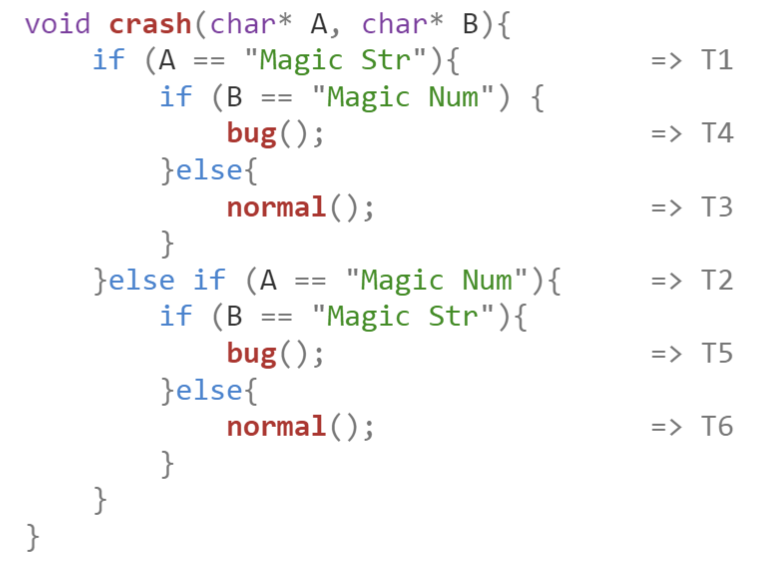
\includegraphics[width=9cm]{crash.png}
    }
    \quad
    \subfloat[]{
        \label{cfg}
        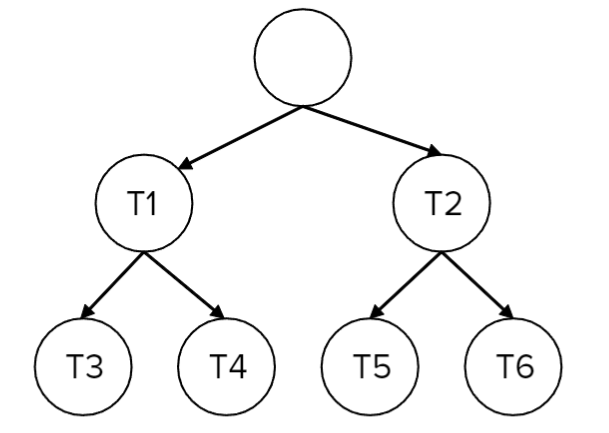
\includegraphics[width=6cm]{cfg.png}
    }
    \caption{异构并行模糊测试优点示例\citing{chen2019enfuzz}(a) crash函数源码;(b) crash函数控制流图}
    \label{motivation}
\end{figure}

通过上述示例可以直观地发现,使用不同模糊测试工具进行模糊测试并相互同步信息能够达到单一模糊测试工具所达不到的效果,不同模糊测试工具算法上的互补能够提高整体的测试效率。

然而Collabfuzz也存在一定的不足,它只能对各个模糊测试实例产生的新的测试用例进行分析,对各个模糊测试实例的执行情况了解有限;并且也只能对测试用例的同步进行调度,调度的粒度较小,对整体并行模糊测试的影响有限。


结合上述对AFL、Ultrafuzz、Collabfuzz的分析,可以得到如表\ref{table1}所示的典型并行模糊测试工具优缺点对比。

\begin{table}[!htbp]
    \caption{典型并行模糊测试工具优缺点对比}
    \begin{tabular}{llll}
    \toprule
    工具& 类型 & 优点 & 缺点 \\
    \midrule
    AFL & 同构并行模糊测试工具 & 系统鲁棒性强 & 存在测试冗余 \\
    Ultrafuzz & 同构并行模糊测试工具 & 不存在测试冗余 & 测试效果存在局限性 \\
    Collabfuzz & 异构并行模糊测试工具 & 整体测试效率高 & 并行调度空间有限 \\
    \bottomrule
    \end{tabular}
    \label{table1}
    \vspace{6pt}
\end{table}

可以看到,对高效并行模糊测试研究还处于起步阶段,各种工具都存在一定程度上的不足,影响了并行模糊测试效率的进一步提升。为此,本文研究优化并行模糊测试的方法,并设计动态策略并行模糊测试系统(Dynamic Strategy Parallel Fuzzer,DSPFuzzer)。

\section{设计目标}
由上一节对现有并行模糊测试方案的分析可知,针对模糊测试的并行化扩展,传统的模糊测试工具的并行模式相比于自身的单实例模式,代码覆盖率上会有一定的提高,但是各模糊测试实例之间同步信息较少,仅定期同步种子文件,不同种子测试的频率存在巨大的差异,导致存在较大的测试冗余,限制了代码覆盖率的进一步提升。同构并行模糊测试工具意图引入主控模糊测试节点,由主控节点统一管理测试任务的分发。这样的好处是避免了模糊测试实例间重复的测试任务执行,提高了并发的力度。但是由于同构并行模糊测试只选择了一种模糊测试算法进行测试,无法充分利用各种技术路线不同的优秀模糊测试算法,导致了一定的测试局限性。异构并行模糊测试集成了不同技术路线的模糊测试工具,使其同时并行执行模糊测试。不同模糊测试技术的差异使得每个模糊测试实例能够为其他实例提供更为有效的新种子,异构化使得模糊测试实例间能够做到优势互补,进而提升整体的测试效率。

但是目前的异构化并行模糊测试的研究仍然存在不足,各模糊测试实例所分配的系统资源相同,相同对待效果较好和效果较差的模糊测试实例会降低整体并行模糊测试的效率;并且未能解决各模糊测试实例维护独立种子池的问题,各模糊测试实例可能会对相同种子进行测试,使得测试存在冗余。

为充分利用并行模糊测试技术在代码路径探索上的优势去挖掘软件的漏洞,本文考虑在已有异构并行模糊测试技术的基础上,通过扩展模块收集更多运行时数据,通过数据指导并行模糊测试系统资源分配和种子挑选,最终提高并行模糊测试的测试效率。本节将从收集细粒度信息、动态分配系统资源和跨实例调度种子三个方面阐述并行模糊测试的研究目标。

(1)收集细粒度信息

现有的异构并行模糊测试方案对模糊测试实例的控制能力较弱,只能控制其同步种子的策略。该局限性产生的原因为并行模糊测试过程中对各模糊测试实例的运行情况了解不足,导致无法收集更多的有效信息数据,从而限制了并行模糊测试的优化。因此需要收集更多并行模糊测试中细粒度运行时数据,来指导并行模糊测试优化算法的提出与实现。

在模糊测试过程中,细粒度的信息收集需要人工在代码中加入探针,而异构并行模糊测试中各个模糊测试实例的实现并不相同,使得需要收集的信息和加入探针的方法都不相同,会增加大量人工参与的工作量。因此对于并行模糊测试中的细粒度信息收集,不追求收集数据的全面性,而是专注于收集重要性程度高、通用性强的数据,这样能尽可能减少从不同模糊测试实例收集到数据的差异性,便于降低数据采集的复杂性和后续的处理难度。此外,还需要降低插入代码的难度,否则不利于扩展新的模糊测试实例,影响系统的可扩展性。

(2)动态分配系统资源

% 模糊测试的测试效率主要包括代码覆盖率的提升效率和崩溃发现的提升效率。代码覆盖率体现了模糊测试对软件测试的完整程度,崩溃发现数体现了模糊测试的最终效果。提高测试效率需要引入优化算法来提升并行模糊测试系统的性能,研究目标1为优化算法提供了数据基础。在已有的数据基础下,本文将从两个独立的角度,分别对已有并行模糊测试方案进行优化。
现有的异构并行模糊测试方案对系统资源的分配不够合理,均等地分配系统资源给不同的模糊测试实例,忽略了模糊测试实例在测试效率上的差异。对于不同的被测软件,各模糊测试实例会有不同的效率。改变不同模糊测试实例的资源分配,会影响整体的测试效率。本系统希望使得测试效率高的模糊测试实例能够执行较多的测试,测试效率低的模糊测试实例能够执行较少的测试,最终提高整体的测试效率。因此本文将对如何通过动态调整不同模糊测试实例的资源分配来提升整体测试效率这一问题进行研究。

(3)跨实例调度种子

现有的异构并行模糊测试方案欠缺对种子调度的能力,模糊测试实例仅分享产生的新种子,具体的测试信息并没有进行分享。因此无法得知同一个种子在不同模糊测试实例中的测试详情。不同的模糊测试实例无法利用全局信息来优化自己的测试策略,可能会产生同一个种子被多个模糊测试实例都大量使用的情况。这种情况可能影响并行模糊测试的效率。因此本文将研究如何在全局视角下评估种子的有效性,进而进行跨实例种子调度。

综上,本文针对并行模糊测试的研究主要包括三个方面:1)收集细粒度信息,提供更多有效信息供并行模糊测试算法优化环节使用;2)动态分配系统资源,让测试效率高的模糊测试实例能够执行更多的测试;3)跨实例调度种子,通过全局管理种子让模糊测试实例能够执行潜在效率更高的种子。

\section{系统方案设计}
为实现本文3.3节中的三个研究目标:收集细粒度信息、动态分配系统资源和跨实例调度种子,本文在Collabfuzz的基础上进行拓展与改进,下面将给出动态策略并行模糊测试整体方案。

\subsection{整体方案设计}
本文设计的动态策略并行模糊测试系统整体方案如图\ref{jiagou}所示。为了支持不同的模糊测试实例,需要在测试之前对被测程序进行针对性的插桩,插桩后的目标程序将被模糊测试实例运行。此外还需要提供初始种子给各模糊测试实例。
\begin{figure}[!htbp]
    \vspace{6pt}
    \centering
    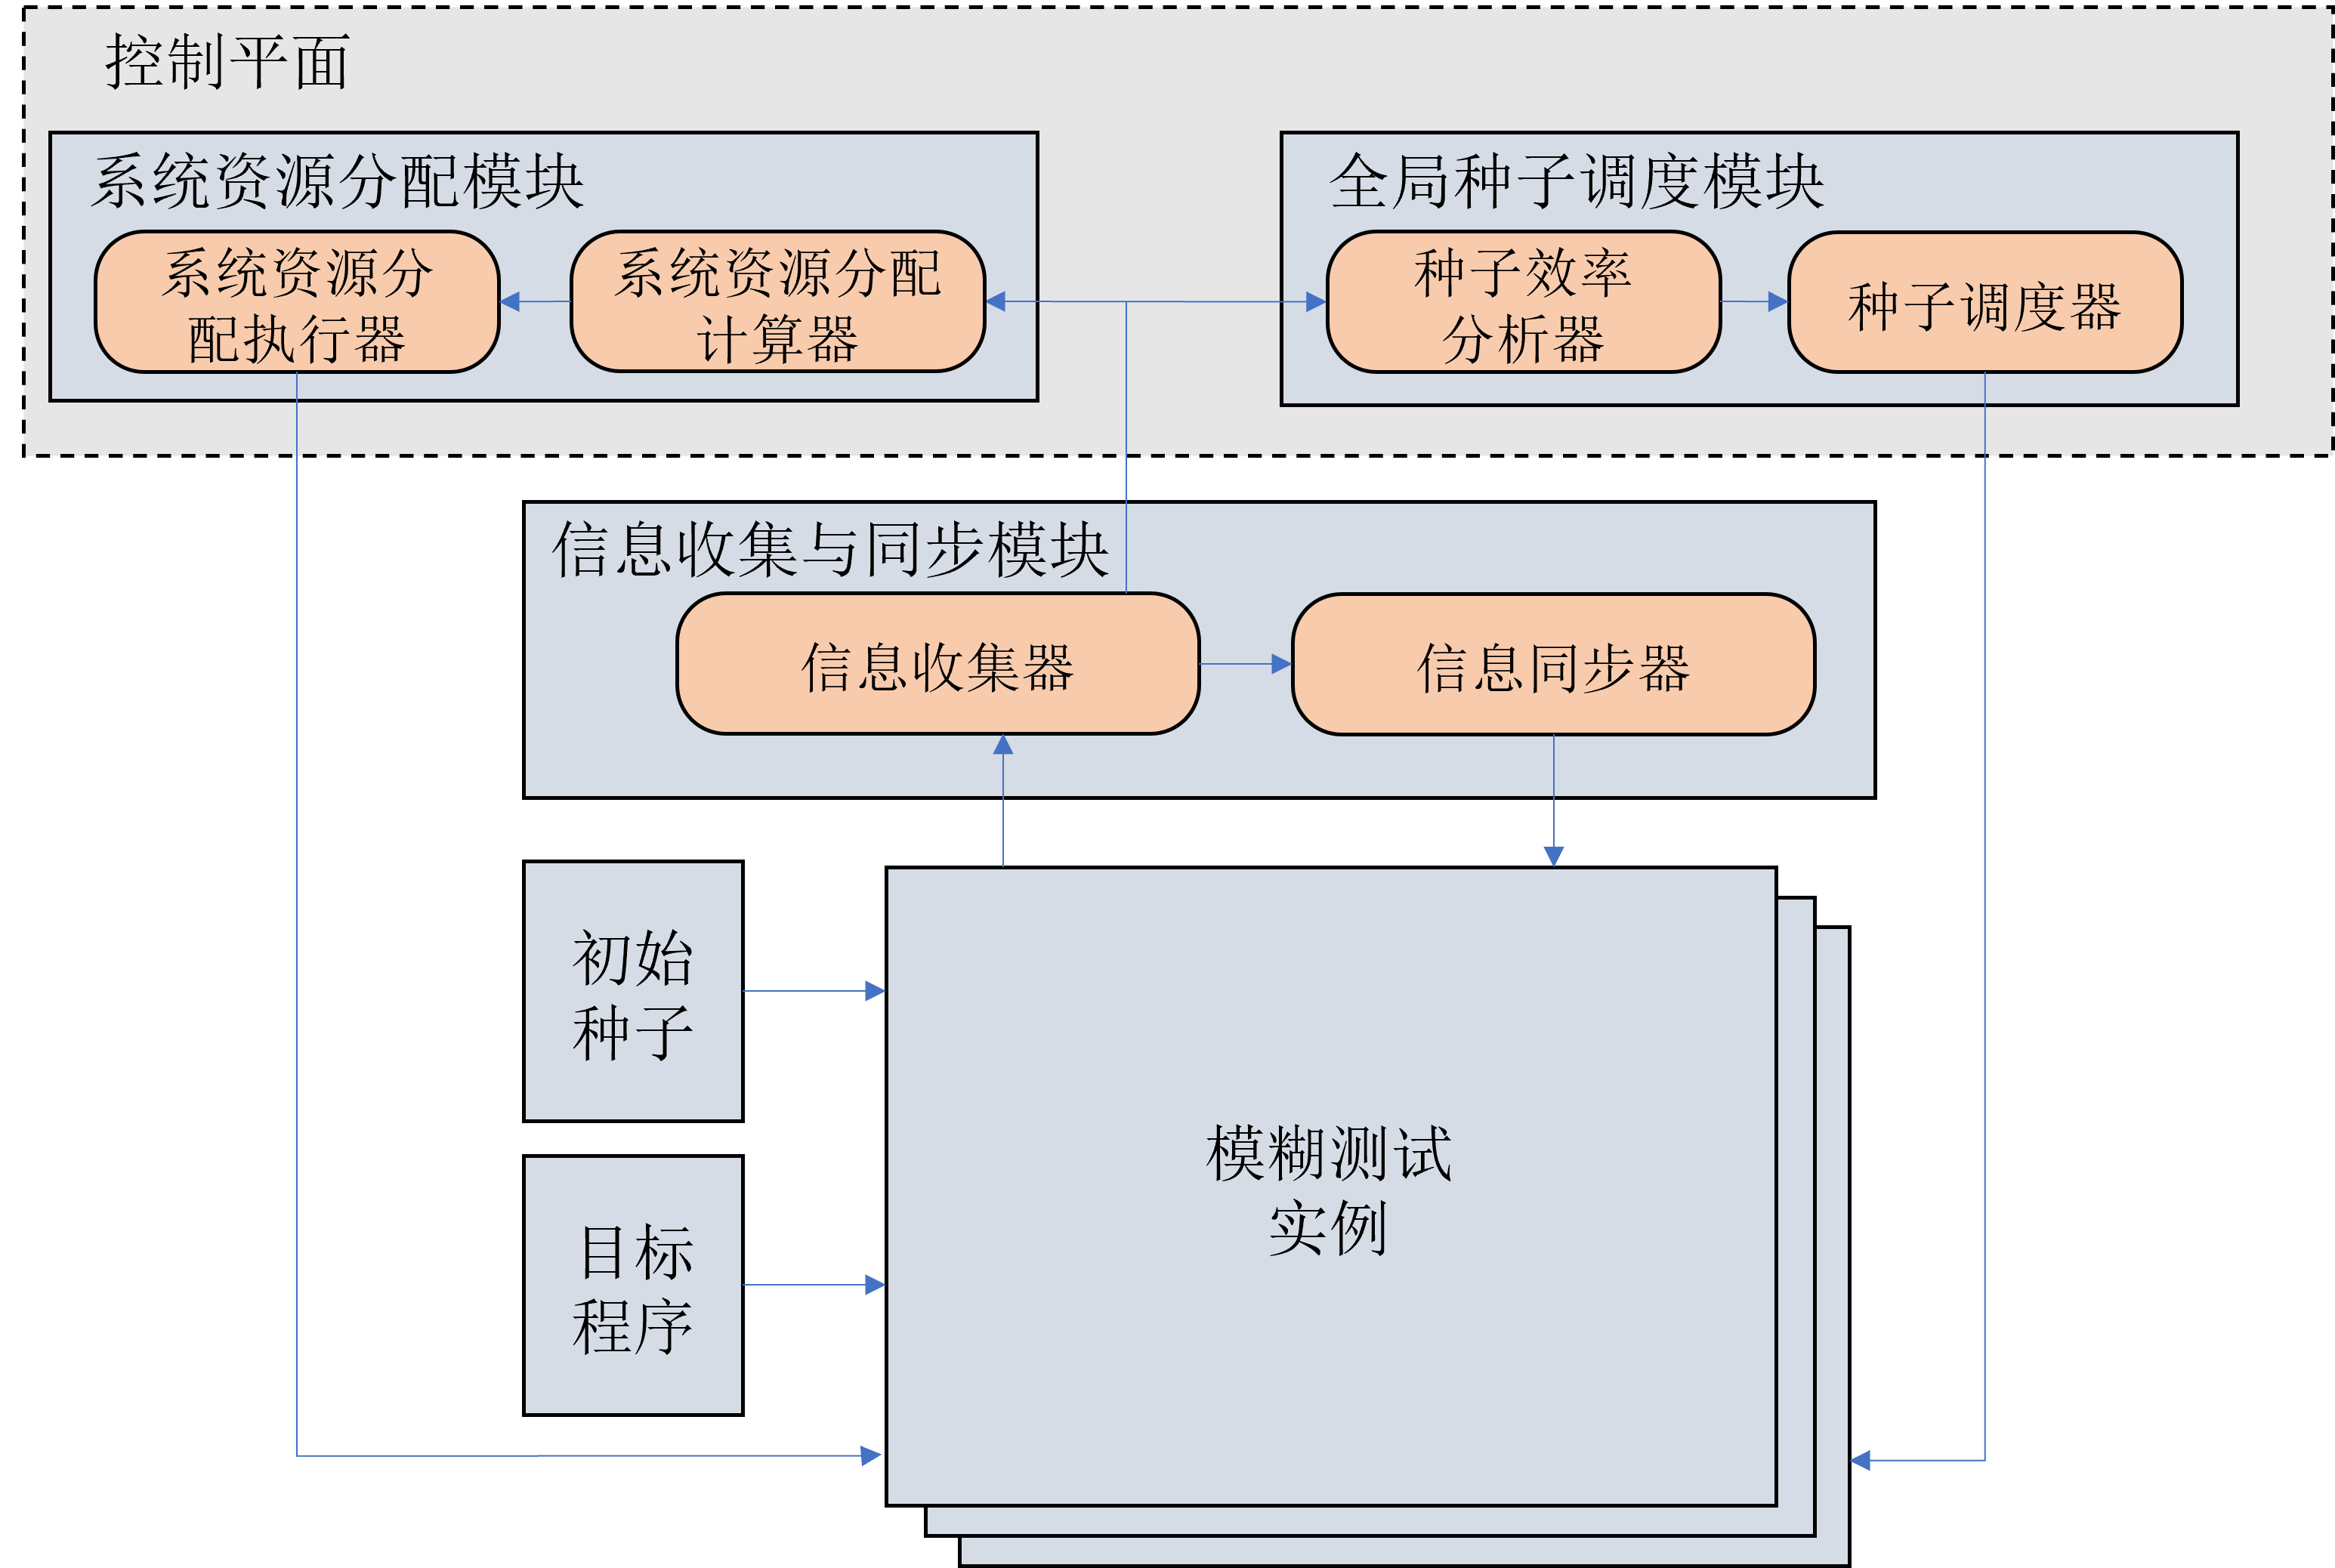
\includegraphics[width=13cm]{jiagou.png}
    \caption{并行模糊测试系统整体方案}
    \label{jiagou}
\end{figure}

针对目标一,为收集细粒度信息,本文设计了信息收集与同步模块。

信息收集与同步模块的难点在于如何挑选并上传所需要收集的信息。首先是这些信息能够对并行模糊测试优化起到指导作用;其次,不同模糊测试工具保存的模糊测试信息各有不同,为了方法的通用性,应该提取各模糊测试工具都维护的信息;最后,不同模糊测试工具的代码实现各有不同,同样是为了模块的通用性,应该设计一种较为通用的获取信息的方法。本文通过对通用模糊测试流程和数据结构的分析,明确了模糊测试过程中通用的有效信息,并且在不改变原有测试流程的情况下,提出了上传所收集信息的方案。

针对目标二,为动态分配系统资源,本文设计了系统资源动态分配模块。

系统资源动态分配模块的难点在于如何决定分配各模糊测试实例的具体资源数值,让未来测试效率高的模糊测试实例能够拥有更多的系统资源,进行更多次的测试,使得整体的测试效率得到提升。为了解决这一难点,先需明确分配系统资源的类型,再研究并行模糊测试中各实例测试效率的关系,得到预测模糊测试实例未来测试效率的方法,并根据该方法的结果对各实例所使用的系统资源进行动态地分配。

针对目标三,为跨实例调度种子,本文设计了跨实例种子调度模块。

跨实例种子调度模块的难点在于如何维护全局的种子状态信息和如何提出一种有效的跨实例种子调度策略。为了解决这些难点,本文设计了专门维护全局种子状态信息的数据结构,使得模糊测试实例能够高效得到所需信息,并且通过研究,发现了种子执行次数与新路径发现概率的关系,进而提出了一种基于种子潜在效率的跨实例种子调度策略。

\subsection{模块功能描述}

在测试开始之前,需要提前准备两种文件:插桩后或原始的目标程序和种子文件。其中,插桩或原始的目标程序是根据模糊测试实例对了解测试情况的需求,定制的可执行二进制文件。种子文件是针对被测程序准备的初始数据。模糊测试实例通过变异种子生成大量测试用例,以探索更多的程序状态空间和发现更多的崩溃。

并行模糊测试系统整体框架包括三部分:信息收集与同步模块、系统资源动态分配模块和跨实例种子调度模块。下面将对这三大模块的功能进行简要描述。

(1)信息收集与同步模块

信息收集与同步模块包括两大部分,信息收集器和信息同步器。信息收集器主要收集两类信息,第一类是模糊测试实例的种子执行情况,该信息需要在模糊测试实例中加入探针代码,在每次种子执行完成之后将当前种子的执行情况记录到日志中,信息收集器通过对日志的收集与整理,得到全局的种子执行情况;第二类是模糊测试实例发现的新种子,监控各模糊测试实例的种子目录,对于新创建的种子文件,计算种子文件的MD5值用于全局种子池的管理,然后判断该种子文件是否具有价值,如果有价值则将该种子文件发送给信息同步器。信息同步器在接收信息收集器发送的种子文件后,将该文件分发到各模糊测试实例的待同步文件队列中。

(2)系统资源动态分配模块

系统资源动态分配模块包括两大部分,系统资源分配计算器和系统资源分配执行器。系统分配计算器首先对信息收集模块整理的不同模糊测试实例种子发现情况进行预处理,得到各模糊测试实例前一个时间段的测试效率,再通过预测模型分析历史测试效率预测得到下一时间段的测试效率,最后将预测的测试效率发送给系统资源分配执行器。系统资源分配执行器通过管理cgroup\citing{ref_cgroup}中的cpu子系统,将预测效率按比例转换成对模糊测试实例所在cgroup组使用CPU资源的限制。

(3)跨实例种子调度模块

跨实例种子调度模块包括两大部分,种子效率分析器和种子调度器。种子效率分析器获取信息收集器收集的全局种子执行情况,根据种子执行次数的多少进行分组,得到每个分组的平均种子执行效率。种子调度器根据不同分组的种子平均效率,计算得出每个种子被选中后的跳过概率,并存入数据库中,模糊测试实例在选择种子之后,会访问数据库,并决定是否跳过当前种子的执行。

\section{本章小结}
本章首先对并行模糊测试的基础模型进行介绍。接下来分析现有并行模糊测试方案的优缺点,并提出了动态策略并行模糊测试系统的三大目标,分别是收集细粒度信息、动态分配系统资源和跨实例调度种子。最后给出了系统的整体框架,并对框架中的信息收集与同步模块、系统资源动态分配模块以及跨实例种子调度模块进行简要介绍。 

\chapter{动态策略并行模糊测试系统关键技术}

本章将介绍并行模糊测试系统的关键技术,首先介绍信息收集与同步技术,包括信息收集技术和信息同步技术的设计与实现;然后介绍系统资源动态分配技术,包括确认需要分配的系统资源、通过预测模型计算系统需分配的资源和系统资源分配功能的实现;最后介绍跨实例种子调度技术,包括确认种子效率与种子执行次数的关系和跨实例种子调度算法的设计与实现。

\section{信息收集与同步技术}

本节首先分析了已有的并行模糊测试算法,梳理了能够进行同步的细粒度信息,并且提出了一种提取这些有效信息的通用方法,然后通过一种中心化的方案实现,提升了同步种子文件的并发度,保证了细粒度信息的可用性。收集的细粒度信息,可以被后续模块使用,为提升并行模糊测试效率提供了基础。

\subsection{信息收集技术}
%明确有效信息,有效信息提取方案
对于细粒度信息收集的任务,首先需要明确哪些信息是需要被收集的,这些信息应该具有通用性,能够被大多数模糊测试工具所利用,否则无法将这些信息的利用扩展到其他模糊测试工具上;其次是采用何种方法收集这些有效信息,收集这些信息的方法也应该具有通用性并且尽可能的简单,这样能够降低测试人员扩展模糊测试工具带来的时间开销。
% \vspace{-20pt}
\begin{algorithm}[t]
    \setstretch{1.3}
    \KwData{$\mathbb{C}$, $t_{limit}$ }
    \KwResult{$\mathbb{B}$ // 发现的Bug集合}
    $\mathbb{B} \leftarrow \varnothing$ \;
    $\mathbb{C} \leftarrow Preprocess(\mathbb{C})$\;
    \While{$Continue(\mathbb{C}, t_{elapsed}, t_{limit})$}{
        $\mathbb{C} \leftarrow \mathbb{C} \bigcup ConfSynchronize()$\;
        $conf \leftarrow Schedule(\mathbb{C}, t_{elapsesd}, t_{limit})$\;
        $tcs \leftarrow InputGen(conf)$\;
        $\mathbb{B}^\prime, execinfos \leftarrow InputEval(conf, tcs, O_{Bug})$\;
        $\mathbb{C} \leftarrow ConfUpdate(\mathbb{C}, conf, execinfos)$\;
        $\mathbb{B} \leftarrow \mathbb{B} \bigcup \mathbb{B}^\prime$\;
    }
    \Return{$\mathbb{B}$}
    \caption{通用并行模糊测试算法}
    \label{parallel_fuzzing}
\end{algorithm}

\vspace{-18pt}
为了更好的分析问题,首先对已有的并行模糊测试算法进行分析。算法\ref{parallel_fuzzing}是一个基于通用模糊测试的并行模糊测试算法\citing{manes2019art},主流模糊测试工具AFL、Angora等都采取了这个算法对自身工具进行了并行化扩展。算法\ref{parallel_fuzzing}以一组模糊测试配置信息 $\mathbb{C}$ 和超时参数 $t_{limit}$ 作为输入,并输出一组发现的Bug(  $\mathbb{B}$)。模糊测试配置信息 $\mathbb{C}$包括被测试程序、提供的初始输入文件等执行模糊测试的必要信息。超时参数 $t_{limit}$决定了模糊测试的总执行时长,到达该时间后模糊测试将自动停止。Bug集合($\mathbb{B}$)可以为测试人员发现程序真正的漏洞提供有效的参考。算法由两部分构成,第一部分是预处理(Preprocess),它在模糊测试流程开始时执行。第二部分是一个循环内的一系列六个方法:配置信息同步(ConfSynchronize)、种子调度(Schedule)、测试用例生成(InputGen)、测试用例评估(InputEval)、配置信息更新(ConfUpdate)和测试终止判断(Continue)。这个循环的每次执行都称为模糊测试迭代。

为了分析模糊测试中信息的通用性,本文进一步分析算法\ref{parallel_fuzzing}具体的步骤:

(1)$\mathbb{C} \leftarrow Preprocess(\mathbb{C})$

测试人员向 $Preprocess$ 提供一组模糊配置作为输入,它返回一组可能被修改的模糊配置。根据模糊测试算法,$Preprocess$ 可以执行各种操作,例如将检测代码插入被测试程序、精简初始种子集合或测量种子文件的执行速度。不同的模糊测试工具根据自身的需求对被检测程序进行插桩,这些插桩方法会带来额外程序运行开销。因此不适合对被测试程序同时进行多种插桩,否则会极大的增加程序的执行时间。

(2)$\mathbb{C} \leftarrow \mathbb{C} \bigcup ConfSynchronize()$

模糊测试工具会定时从其他模糊测试工具获取配置信息并与自身的配置信息进行整合。由于是主动从其他模糊测试工具处获取信息,因此只能获取到可持久化的信息,这些信息通常是以文件形式保存的新发现的种子。模糊测试工具会对其他模糊测试工具新发现的种子进行评估,将有效的种子添加到自身的种子队列中。

(3)$conf \leftarrow Schedule(\mathbb{C}, t_{elapsesd}, t_{limit})$

$Schedule$ 将当前的模糊配置集、当前时间和测试超时时间作为输入,生成用于当前模糊测试迭代的模糊配置。$conf$ 通常包括调度选择的种子,种子的能量等信息。不同的模糊测试工具根据自身的目标设计了不同的种子调度策略。

(4)$tcs \leftarrow InputGen(conf)$

$InputGen$将当前迭代模糊配置($conf$)作为输入,并返回一组具体的测试用例($tcs$)作为输出。基于变异的模糊测试工具使用$conf$中的种子来生成测试用例,基于生成的模糊测试工具使用模型或语法作为参数。基于变异的生成方式可能会利用一些已知信息,如输入字节与程序分支的映射关系,不同变异算子的变异效率等信息。但是这些信息仍然不够通用,输入字节与程序分支映射关系取决于使用何种预处理方法,并且不一定能保证精准性和有效性,不同模糊测试工具使用的变异算子种类也不尽相同。

(5)$\mathbb{B}^\prime, execinfos \leftarrow InputEval(conf, tcs, O_{Bug})$

$InputEval$将模糊配置$conf$、一组测试用例$tcs$ 和一个错误预言机($O_{Bug}$) 作为输入。它将测试用例($tcs$)输入给被测试程序,并执行被测试程序,使用$O_{Bug}$(假设已经集成到模糊测试工具中,如程序异常中止)检查执行是否违反了安全策略。然后它输出发现的Bug集合($\mathbb{B}^\prime$)和有关模糊测试运行的执行情况信息($execinfos$),这些信息可用于更新模糊测试配置。Bug集合已经是模糊测试的最终输出信息,无需额外同步给其他模糊测试工具。执行情况信息包括通用信息与各模糊测试工具用于自身算法的特色信息。对于灰盒模糊测试来说,通用信息的代表为该种子变异的次数、变异生成的有效种子数等,这些是每个灰盒模糊测试工具都会直接或间接维护的信息。执行情况特色信息与模糊测试工具使用的优化策略有关,如表\ref{table_info}所示,Mopt会收集测试时不同变异算子生成有效种子的数量并统计它们的效率,Tortoisefuzz会收集每次测试时被测试程序执行危险指令的数量。

\begin{table}[!htbp]
    \caption{模糊测试工具特色信息}
    \begin{tabular}{llll}
    \toprule
    模糊测试工具& 特色信息 \\
    \midrule
    AFLFast & 路径频率 \\
    Fairfuzz & 变异掩码 \\
    Mopt & 变异算子效率 \\
    Tortoisefuzz & 种子执行到潜在漏洞的数量 \\
    Angora & 输入字节流与程序结构映射关系 \\
    Savior & 包含潜在漏洞的全局控制流图 \\
    \bottomrule
    \end{tabular}
    \label{table_info}
    \vspace{6pt}
\end{table}

(6)$\mathbb{C} \leftarrow ConfUpdate(\mathbb{C}, conf, execinfos)$

$ConfUpdate$将一组模糊配置$\mathbb{C}$、当前配置 $conf$ 以及有关每个模糊用例的运行信息($execinfos$)作为输入。它可能会更新模糊配置集$\mathbb{C}$。例如,许多灰盒模糊测试工具根据$execinfos$减少$\mathbb{C}$中模糊配置的数量。模糊配置$\mathbb{C}$也会含有一些与具体模糊测试相关的特色信息,这些信息有助于实现更好的调度策略和用例生成策略。如表\ref{table_info}所示,AFLFast维护了种子对应的路径频率信息,Fairfuzz维护了低频分支来生成变异掩码,Mopt维护了变异算子的效率信息,Tortoisefuzz维护了种子对应的危险指令执行数量,Angora维护了输入字节流与程序结构的映射关系,Savior维护了一个包含潜在漏洞的全局控制流图。这些信息都与自身的模糊测试策略有紧密的联系。

(7)$\{True, False\}\leftarrow Continue(\mathbb{C}, t_{elapsed}, t_{limit})$ 

$Continue$ 将模糊配置$\mathbb{C}$、测试运行时间和测试终止时间作为输入,输出一个布尔值,指示是否应进行新的模糊测试迭代。对于白盒模糊测试来说,当没有更多路径可供发现时,可以终止测试。对于灰盒模糊测试来说,通常存在一个中止时间,如24小时,达到中止时间后测试结束。

通过上述对并行模糊测试流程的分析,可以发现不同的模糊测试工具根据自己的设计目标,维护了许多特有的信息为算法实现提供支撑,这些信息难以直接被其他模糊测试工具利用。因此为了使得提取的信息能够被其他模糊测试工具利用上,应该收集每种模糊测试工具中都生成并利用的数据。根据上述分析,除了现有方案中同步的种子文件,对每个种子的执行次数和通过该种子变异生成新的有效种子的数量也是一种值得同步的信息,后续章节将展示如何利用这种信息提高系统的测试效率。

\begin{algorithm}[!htbp]
    \setstretch{1.3}
    \KwData{$\mathbb{C}$, $t_{limit}$ }
    \KwResult{$\mathbb{B}$ // 发现的Bug集合}
    $\mathbb{B} \leftarrow \varnothing$ \;
    $\mathbb{C} \leftarrow Preprocess(\mathbb{C})$\;
    \While{$Continue(\mathbb{C}, t_{elapsed}, t_{limit})$}{
        $\mathbb{C} \leftarrow \mathbb{C} \bigcup ConfSynchronize()$\;
        $conf \leftarrow Schedule(\mathbb{C}, t_{elapsesd}, t_{limit})$\;
        $tcs \leftarrow InputGen(conf)$\;
        $\mathbb{B}^\prime, execinfos \leftarrow InputEval(conf, tcs, O_{Bug})$\;
        $\mathbf{ConfUpload(conf, execinfos)}$\;
        $\mathbb{C} \leftarrow ConfUpdate(\mathbb{C}, conf, execinfos)$\;
        $\mathbb{B} \leftarrow \mathbb{B} \bigcup \mathbb{B}^\prime$\;
    }
    \Return{$\mathbb{B}$}
    \caption{通用并行模糊测试算法优化}
    \label{parallel_fuzzing_pro}
\end{algorithm}

确定好所需提取的有效信息之后,应该明确一种提取这些数据的方法。由于这些数据属于程序运行中的内部数据,因此只能通过人工修改代码的方式将这些数据提取出来。由于各模糊测试工具实现方法不同,为保证本文系统对于模糊测试实例的可扩展性,提取数据的方法应该尽可能的通用、简单,应该作为一个环节,添加到已有的算法逻辑中。根据对算法\ref{parallel_fuzzing}的流程分析,在一次测试迭代中按顺序经历了种子调度、测试用例生成、测试用例评估、配置信息更新和测试终止判断等过程。为了提取信息,应该在配置信息更新之前,将当前迭代的测试信息同步出去。算法\ref{parallel_fuzzing_pro}描述了这种在已有并行模糊测试算法下增加细粒度信息提取的方法。由于希望同步的数据为种子的执行次数和通过该种子变异生成新的有效种子的数量,更为具体的做法是在种子调度环节之后、测试用例生成环节之前,统计当前模糊测试总的执行次数和总的种子数量,再在测试用例评估环节之后统计这两个数据,它们的差值就是当前种子的执行次数和通过该种子变异生成新的有效种子的数量。

\subsection{信息同步技术}
%已有问题,解决方案,去重

上一小节提出了一种针对细粒度信息收集的并行模糊测试算法,但是在实际工程实现上,仍然存在一些需要解决的问题,如提升同步种子文件的并发度、保证细粒度信息的可用性。

AFL的并行模糊测试算法实际上是一个去中心化的架构,每个模糊测试工具会定时同步其他模糊测试工具的种子文件,因此需要扫描各个模糊测试工具存放种子文件的种子目录。然而在同步阶段扫描目录是不可扩展的:首先,用于发现新的、未同步的测试用例的目录枚举操作的数量随着模糊测试工具数量的增加呈非线性增加,这导致同步阶段的耗时更长。例如,每个模糊测试实例将采用 $O(f*t)$,其中 $f$ 是模糊测试实例的数量,$t$ 是测试用例目录中测试用例的数量;其次,目录枚举严重干扰了创建新测试用例,因为目录写操作(即创建文件)和读操作(即枚举文件)不能同时执行\citing{min2016understanding}。由于每个模糊测试实例的内部信息不共享,这种去中心化的架构导致信息存在冗余,因此每个模糊测试实例都需要完整扫描除它本身维护的种子文件之外的所有种子文件。从另一个角度看,每个种子文件,都将被扫描$f-1$次。并不是每个种子文件对于其他模糊测试都是有价值的。为了减低模糊测试工具对种子文件频繁扫描的次数,可以使用一种中心化的架构,通过统一的管理种子文件,在中心节点评估每个种子对不同模糊测试实例是否有价值,如果有价值,再分发到对应的同步队列中,模糊测试实例只从对应的同步队列中同步种子文件,减轻同步种子文件带来的对并发度的影响。

针对第二个问题,由于一个模糊测试实例上传的细粒度信息并不能够直接被其他模糊测试实例使用,因此也需要一个中心化数据库来保存这些细粒度信息。此外,同一个种子文件可能存在于不同模糊测试实例的种子队列中,它们的细粒度执行信息应该进行整合,否则无法根据这些细粒度信息做跨实例种子调度。因此如何识别出这些相同的种子文件,也是一个需要解决的问题。由于同步后的种子文件内容相同,因此对种子文件做哈希计算也会得到相同的结果,因此本系统将在模糊测试实例中额外保存每个种子文件创建时的MD5值,这个值也将和种子执行信息一起上传,作为区分不同种子的唯一标识。

\begin{figure}[!htbp]
    \vspace{6pt}
    \centering
    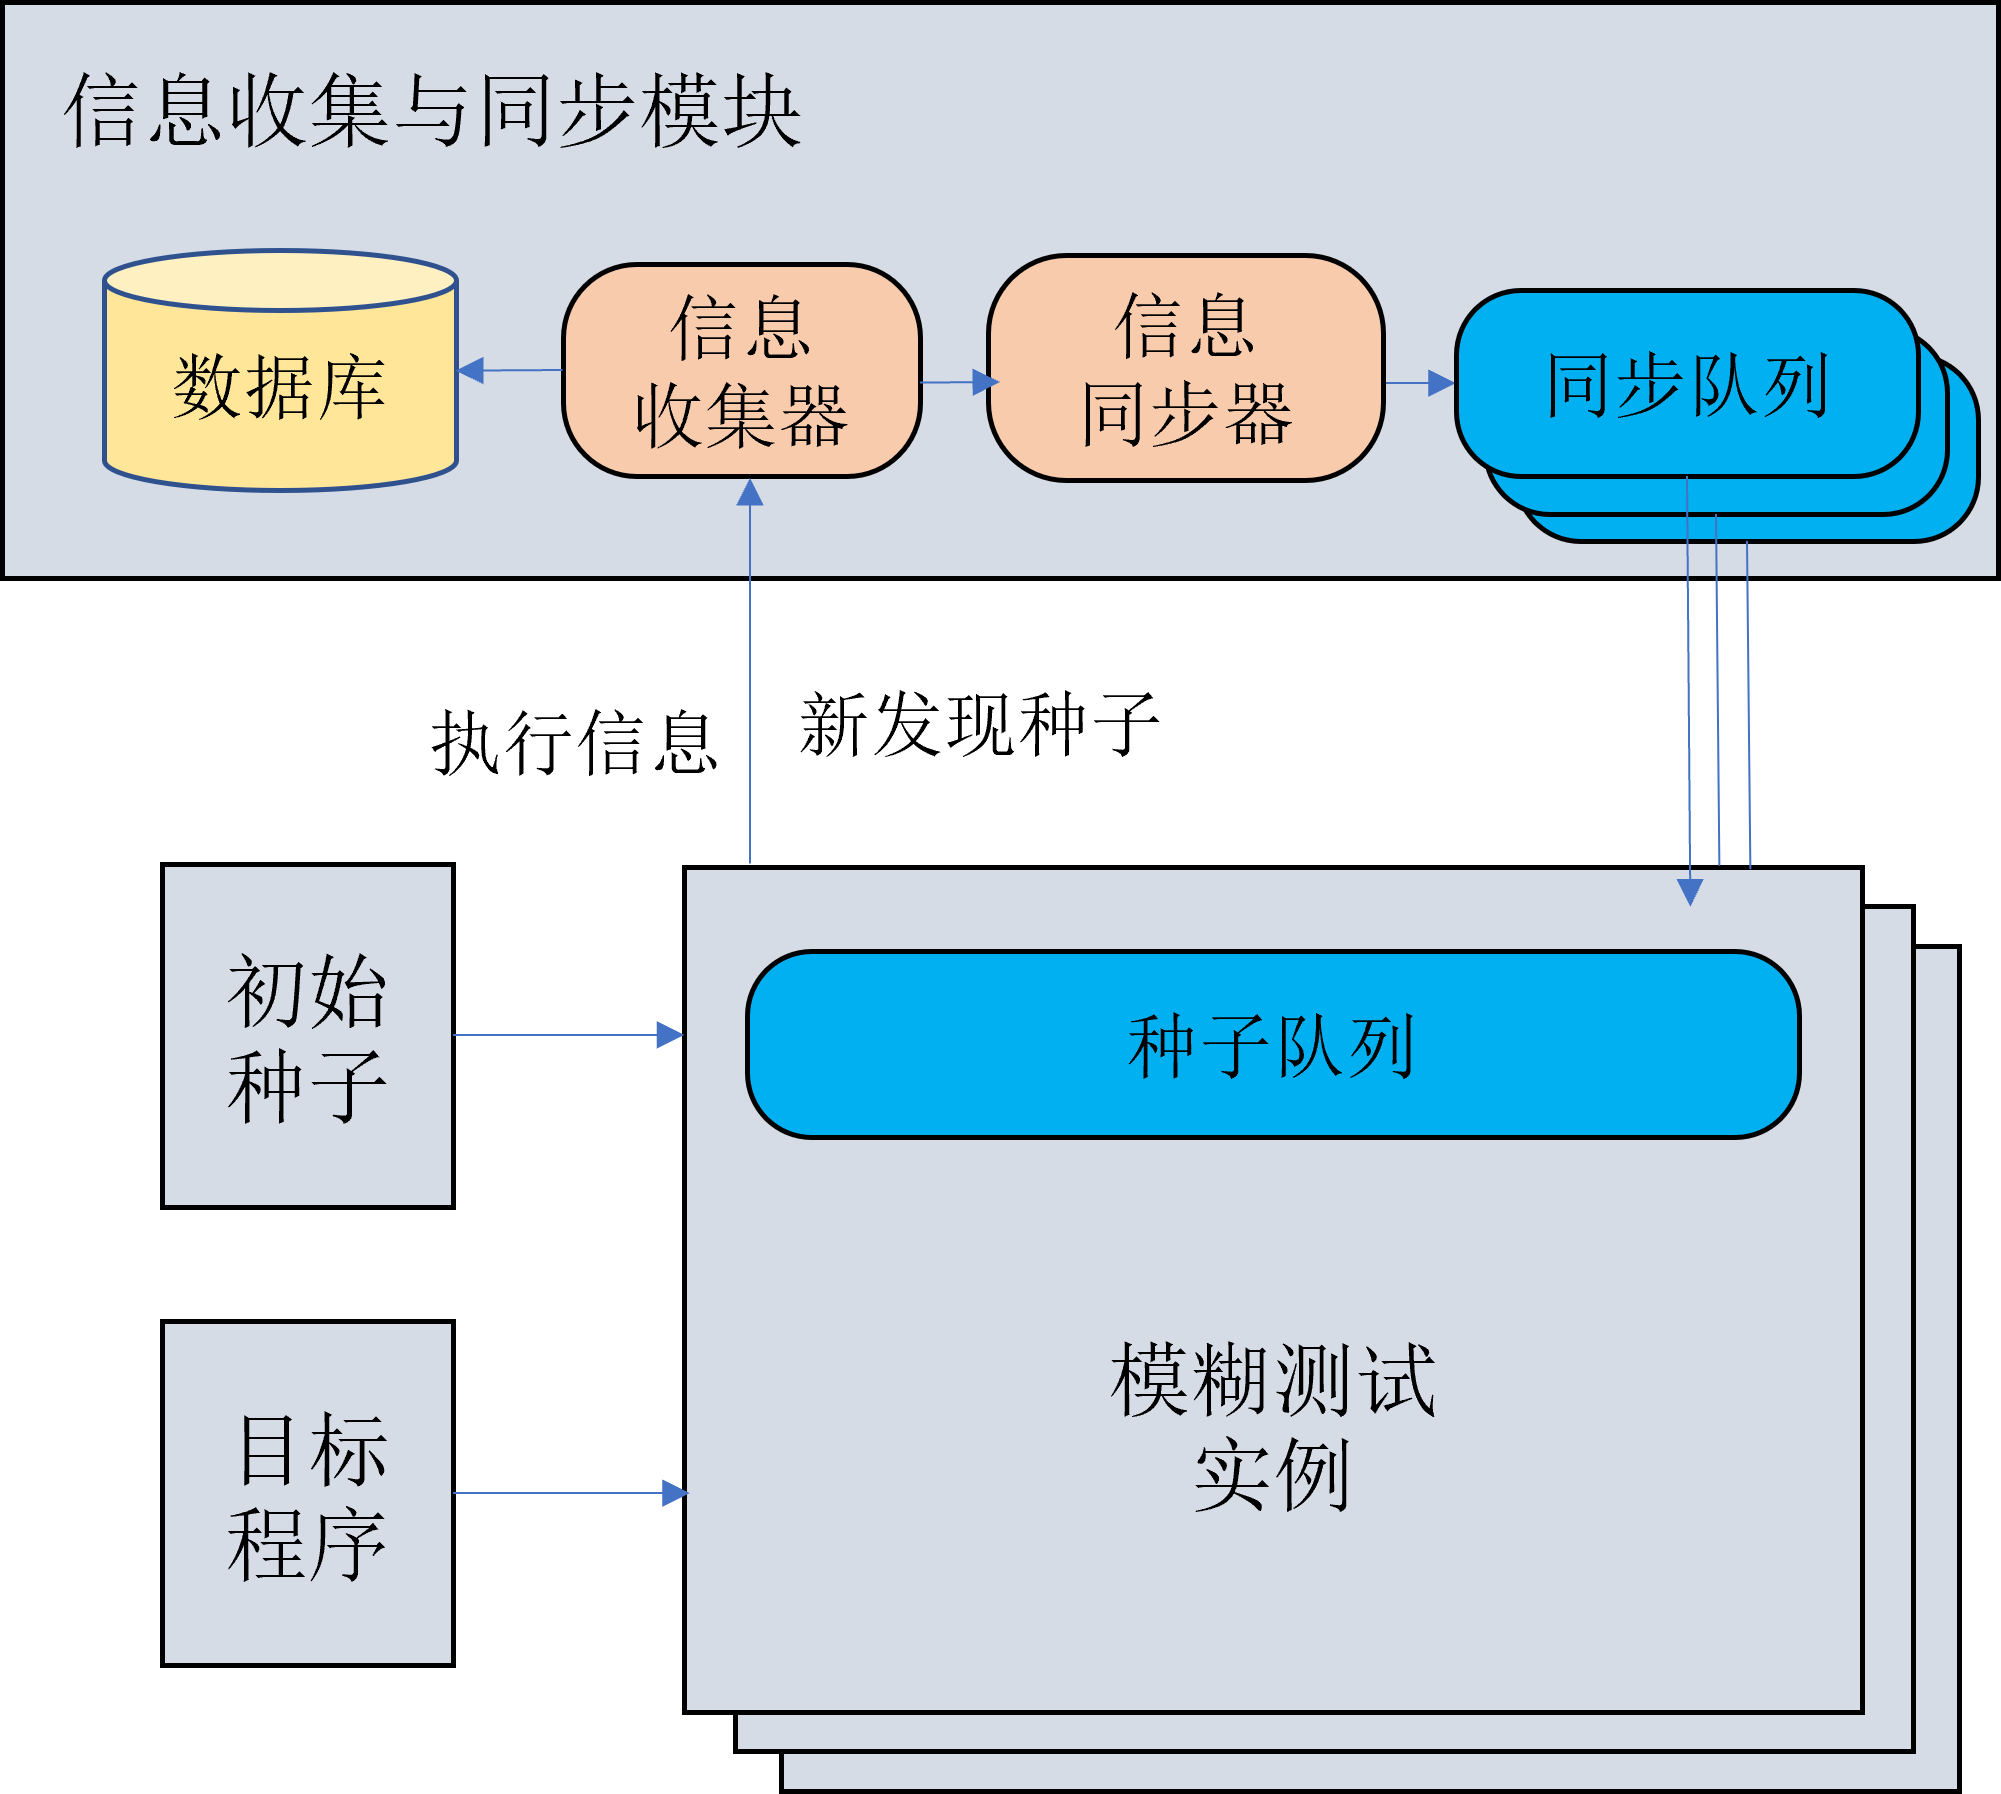
\includegraphics[width=9cm]{syn.png}
    \caption{信息获取与同步架构}
    \label{syn}
\end{figure}

图\ref{syn}展现了本文系统中完整的信息收集与同步模块,在每次模糊测试实例执行完一次迭代中的测试用例评估后,如果有新生成的种子,则将这些种子上传给信息同步模块,进行分析,再按照需求分发到不同的同步队列中,对于当前种子的执行数量和发现新种子的数量,则与该种子的MD5值一同储存到数据库中,待后续的使用。表\ref{table_database}介绍了数据库各个字段的名称、类型与作用,$seed\_id$是种子的MD5哈希值,通过字符串形式进行保存,$exec\_nums$是种子的总执行数量,通过32位有符号整型数进行保存,$find\_nums$是种子发现新种子的数量,通过32位有符号整型数进行保存,$eff$是种子的潜在效率,通过8位无符号整型进行保存,其中$eff$字段的设置将在4.3.2小结进行介绍。


\begin{table}[!htbp]
    \caption{数据库字段}
    \begin{tabular}{lll}
    \toprule
    字段 & 类型 & 作用 \\
    \midrule
    seed\_id & STRING & 种子唯一标识符 \\
    exec\_nums & INT32 & 种子执行数量 \\
    find\_nums & INT32 & 发现新种子的数量 \\
    eff & UINT8 & 种子的潜在效率 \\
    \bottomrule
    \end{tabular}
    \label{table_database}
    \vspace{6pt}
\end{table}

\section{系统资源动态分配技术}

对模糊测试实例使用的系统资源进行动态分配是希望让整体测试效率更高,这里的潜在前提是不同模糊测试工具对不同软件进行测试时的效果存在差异。这里的差异主要体现在两个维度:对于不同软件的测试结果来说,不同模糊测试工具对不同软件的测试效果存在差异;对于同一款软件的测试完整过程来说,模糊测试工具的测试效率也随测试时长的变化而变化。

文献\cite{li2021unifuzz}评估了8款主流的模糊测试工具,观察到以下结果:对于 20 个真实世界的程序,QSYM 在五个程序上表现最好。Angora 、Honggfuzz\citing{honggfuzz} 和 Mopt 分别在三个程序上表现最好,AFL 在一个程序上表现最好。体现了第一个维度的差异。此外该文献还发现模糊测试工具性能之间的比较可能会随着时间的推移而发生逆转。例如,Mopt 在早期对程序 sqlite3 发现的独特崩溃少于 QSYM,但在 10 小时后发现的独特崩溃比 QSYM 多。体现了第二个维度的差异。

为了提高测试效率,一个直观的想法是让当前测试效率高的模糊测试实例拥有更多的系统资源,提高测试速度,间接提高整体的测试效率。为了实现上述目的,本节将依次介绍如何确定需要动态分配的系统资源、如何预测模糊测试实例未来的测试效率、如何设计分配算法和功能的具体实现。

\subsection{系统资源选择}

为了得到适用于并行模糊测试系统的系统资源动态分配算法,首先需明确需要对何种系统资源进行动态分配。在并行模糊测试中,主要使用到的系统资源有CPU、内存、硬盘和网络。接下来将依次分析这些系统资源的动态调整对模糊测试有何影响。

(1)CPU

在模糊测试中,CPU主要用于测试用例生成和程序执行。模糊测试的核心是生成各种不同的测试用例,而测试用例的生成通常需要使用大量的 CPU 资源。测试用例生成的过程可能涉及到各种算法和技术,如遗传算法、污点分析等,这些都需要进行大量的计算。生成的测试用例需要在被测程序中进行执行,并且需要监控程序的运行状态。程序执行时需要使用大量的 CPU 资源,尤其是在测试复杂程序时,需要更高性能的 CPU。通过上述分析,可以发现CPU资源将直接影响模糊测试的速度,更多的CPU资源意味着在单位时间内模糊测试工具能够执行更多的指令,生成更多的测试用例,执行更多的测试。

(2)内存

在模糊测试中,内存主要用于生成测试用例和程序执行时的状态信息。测试用例的生成通常是通过对已有测试用例进行修改或组合得到的,这涉及到对测试用例进行存储和处理。在测试用例生成的过程中,需要保存生成的测试用例,并且在进行组合或修改时,需要将不同的测试用例加载到内存中进行处理。程序执行时,需要将程序和测试用例同时加载到内存中,并且程序执行过程中产生的日志、堆栈和内存信息也需要保存到内存中。如果程序比较复杂,测试用例数量又较多,那么所需的内存资源就会非常大。通过上述分析可以发现,内存也是影响模糊测试效率的一个重要资源。与CPU资源不同的是,当可用内存较少时,内存资源将成为模糊测试的瓶颈,可能会造成生成测试用例过慢和程序执行异常崩溃的情况。但当内存资源充足时,模糊测试不会因为可用内存的增加而直接提升效率。对于现代操作系统来说,内存的大小通常足够模糊测试使用,因此对内存的动态分配不会对模糊测试的执行效率有明显的影响。

(3)硬盘

在模糊测试中,硬盘空间主要用于存储测试用例、程序执行结果、日志和其他调试信息。测试用例需要存储在硬盘上以备后续的测试,而程序执行过程中产生的日志和崩溃信息也需要保存在硬盘上,以便进行分析和调试。测试用例数量、大小和程序的复杂度都会影响硬盘空间的使用量。过度使用硬盘空间可能会导致系统性能下降,因此可以对硬盘空间的使用进行优化和控制,例如定期清理无用的测试用例和测试日志等。通过上述的分析可以发现,随着模糊测试的进行,对硬盘的需求将不断增大。与内存资源一样,硬盘资源也是在不足的情况下会影响模糊测试的进行,如无法储存更多的有效种子。当硬盘资源充足时,硬盘空间的提升并不会提高模糊测试的速度。并且硬盘作为可扩展性较强的系统资源,通常有较大的余量供用户使用。

(4)网络

在同一个主机进行并行模糊测试,通常不涉及网络资源的使用,但如果是使用不同主机进行并行模糊测试,网络资源的使用就非常必要了。在这种情况下,需要确保测试主机之间能够互相通信并共享资源,例如共享种子文件和执行路径等信息。同时,还需要保证网络的稳定性和带宽的充足,否则同步过程中的网络延迟和丢包等问题会直接拖慢模糊测试的速度。与内存和硬盘资源一样,网络资源的不足会成为并行模糊测试系统的瓶颈,但是充足的网络资源并不会使得并行模糊测试获得额外的增益。

\begin{table}[!htbp]
    \caption{模糊测试使用的系统资源}
    \begin{tabular}{ll}
    \toprule
    系统资源类别 & 主要用途 \\
    \midrule
    CPU & 生成大量的随机输入数据、运行待测试程序 \\
    内存 & 运行待测试程序 \\
    硬盘 & 储存测试结果 \\
    网络 & 同步测试信息 \\
    \bottomrule
    \end{tabular}
    \label{table_resource}
    \vspace{6pt}
\end{table}

通过对上述四种被并行模糊测试使用的系统资源的分析可以发现,CPU资源直接影响模糊测试的速度,给模糊测试实例分配更多的CPU资源,可以提高模糊测试的执行速度。而对于内存、硬盘、网络这三种资源资源,当这些资源不足时,会成为并行模糊测试的瓶颈,影响测试速度或影响测试结果。然后当资源的分配已经达到并行模糊测试的使用需求时,提供额外更多的系统资源将不再能提升系统的测试速度。此外,CPU资源通常是有限且不易于扩展的。而其他系统资源相对于CPU资源来说,扩展相对容易。综上所述,CPU是一种直接影响并行模糊测试测试效率的系统资源,可以将这种资源动态分配给不同的模糊测试实例,以试图提高并行模糊测试的效率。

% 介绍模糊测试使用的系统资源;
% 分析该使用何种系统资源
% 说明模糊测试工具的效率使动态变化的,因此需要一个预测模型
% 提出预测模型并选择最合适的模型
% 具体的工程算法实现

\subsection{效率预测技术}

在确定好需要动态分配的资源后,接下来研究如何预测模糊测试实例的测试效率,首先需要对问题进行数学上的建模。

模糊测试可以看作一个时间连续的随机过程。为了便于后续的分析,本文将使用一个固定的时间窗口对模糊测试的效果进行评估,将时间连续的过程转化为时间离散的过程。具体对各模糊测试实例效果评估的指标定位新发现种子的数量,在一段时间内发现的种子数量越多,说明这段时间内模糊测试实例的效率越高。由于在模糊测试过程中,不同时间段的测试效果存在明显差异,通常变现为模糊测试前期发现种子的速度快,而后期发现种子的速度较慢。为了使得数据能够被算法统一处理,需要对其进行归一化,即每个模糊测试实例的效率为 $x_{i, t} = a_{i,t} / A_t$,$a_{i,t}$为第$i$个模糊测试实例在第$t$个时间段内发现种子的数量,$A_t$为所有模糊测试实例在第$t$个时间段内发现种子的数量。则第$t$个时间段各模糊测试实例的效率可表示为$X_t = \{x_{1, t}, x_{2, t}, ..., x_{m, t}\}$,$m$为模糊测试实例的数量。当前的任务变成了在已知 $\{X_1, X_2, ..., X_t\}$ 的情况下,预测下一个($t + 1$)时间段的模糊测试效率($X_{t + 1}$)。

将上述建模进行转换,本质上是将观测对象按照时间顺序排列,构成一个时间序列,从已有的时间序列中总结变化规律,推断今后变化的可能性。这是一个典型的时间序列模型。

时间序列模型是一种回归模型,其基于的原理是,一方面承认事物发展的延续性,运用过去时间序列的数据统计分析就能推测事物的发展趋势;另一方面又充分考虑到偶然因素影响而产生的随机性,为了消除随机波动的影响,利用历史数据,进行统计分析,并对数据进行适当的处理,进行趋势预测。

由于时间序列模型具有多种具体的实现模型,本文将介绍三种最为常见的模型:自回归模型、滑动平均模型和自回归滑动模型。

(1)自回归模型

自回归模型(Autoregressive Model,AR Model),是统计上一种处理时间序列的方法,用同一变数例如$x$的之前各期,亦即$x_1$至$x_{t-1}$来预测本期$x_t$的表现,并假设它们为线性关系。因为这是从回归分析中的线性回归发展而来,只是不用 $x$预测 $y$ ,而是用 $x$ 预测 $x$;所以叫做自回归。

更进一步,如果时间序列中的每个数据都为一个向量,则该模型被称之为多维自回归(Vector Autoregression,VAR)模型,其计算公式如下:
\begin{equation}
    X_t = c + \sum_{i=1}^{p} A_i X_{t-i} + \epsilon_t
\end{equation}

其中,$X_t$ 是一个 $k$ 维列向量,表示在时刻 $t$ 的观测值。$p$ 是模型的滞后阶数,是VAR模型重要的参数,$A_i$ 是一个 $k \times k$ 的系数矩阵,表示在时刻 $t-i$ 的观测值对当前观测值的影响。$\epsilon_t$ 是一个 $k$ 维列向量,表示在时刻 $t$ 的误差。

$c$ 是一个 $k$ 维列向量,表示常数项。如果不考虑常数项,则将 $c$ 设为 $0$。

% Vector Autoregression(VAR)模型中,最小二乘法(Ordinary Least Squares,OLS)是估计模型系数的一种方法,其具体算法如下:

% 假设有 $m$ 个变量,$p$ 个滞后期,有 $N$ 个时间步长的样本数据,$Y_t$ 是一个 $m$ 维列向量,表示在时间 $t$ 的 $m$ 个变量的取值,$X_t$ 是一个 $mp$ 维矩阵,表示 $m$ 个变量的 $p$ 个滞后期的值。

% 首先,将 VAR 模型转换为 OLS 模型,即 $Y_t = X_t B + \epsilon_t$,其中 $B$ 是一个 $mp \times m$ 维矩阵,表示模型的系数,$\epsilon_t$ 是一个 $m$ 维列向量,表示模型的误差项。

% 然后,通过最小二乘法(OLS)来估计系数 $B$。具体来说,我们要求解下面的正规方程:

% $$X^{\prime}X\hat{B}=X^{\prime}Y$$

% 其中,$\hat{B}$ 是系数矩阵的估计值,$X\prime$ 是矩阵 $X$ 的转置。解出 $\hat{B}$ 后,就可以得到 VAR 模型的系数,从而进行预测和分析。

VAR模型中,最小二乘法(Ordinary Least Squares,OLS)是估计模型系数的一种常用方法,在实际应用中,VAR 模型通常需要进行多次迭代才能得到最优的系数估计值。此外,如果模型中存在共线性或高度相关的变量,OLS 估计的系数可能会不准确或不稳定。因此,在实际应用中,需要结合领域知识和其他方法(如 Lasso、Ridge 等)来对模型进行进一步的调整和优化。

(2)滑动平均模型

滑动平均(Moving Average,MA)模型也是一种常见的时间序列分析方法之一,用于预测时间序列的未来值。滑动平均模型的核心思想是通过对时间序列的残差进行建模来进行预测。

MA 模型的建立通常包括三个步骤:确定阶数,估计参数和模型检验。在确定阶数时,需要通过观察自相关函数和偏自相关函数的图形来判断模型的阶数。在估计参数时,常用的方法是最大似然估计。在模型检验时,需要检查模型的残差序列是否符合白噪声的特征,如果存在自相关性则需要对模型进行调整。

MA 模型有两个重要的参数:阶数和移动平均窗口。MA 模型中的阶数通常用 $q$ 表示。移动平均窗口指的是在计算残差序列的平均值时,用到的观测值的个数,通常用 $m$ 表示。

更进一步,如果时间序列中的每个数据都为一个向量,则该模型被称之为多维滑动平均(Vector Moving Average,VMA)模型,其计算公式如下:

设 $X_{t}$ 是一个 $m$ 维时间序列,$W_{1},W_{2},\cdots,W_{q}$ 是一个权重系数序列,则多维滑动平均模型可以表示为:
\begin{equation}
    X_{t} = W_{1}\varepsilon_{t-1} + W_{2}\varepsilon_{t-2} + \cdots + W_{q}\varepsilon_{t-q} + \mu 
\end{equation}


其中,$\varepsilon_{t-1},\varepsilon_{t-2},\cdots,\varepsilon_{t-q}$ 是 $m$ 维的白噪声序列,$\mu$ 是常数。

可以将上述公式转化为矩阵形式:
\begin{equation}
    X_t = \boldsymbol{W}\boldsymbol{\varepsilon}_{t} + \boldsymbol{\mu}
\end{equation}

其中,$X_t = [x_{1,t},x_{2,t},\cdots,x_{m,t}]^{\top}$,$\boldsymbol{\varepsilon}_{t} = [\varepsilon_{1,t},\varepsilon_{2,t},\cdots,\varepsilon_{q,t}]^{\top}$,$\boldsymbol{\mu} = [\mu,\mu,\cdots,\mu]^{\top}$,$\boldsymbol{W}$ 是一个 $m \times q$ 的矩阵,表示滑动平均模型的权重系数,其中第 $i$ 行第 $j$ 列的元素 $w_{i,j}$ 表示 $x_{i,t-j}$ 对 $x_{t}$ 的影响。

多维滑动平均模型可以通过最小二乘法进行参数估计。如果假设误差项 $\boldsymbol{\varepsilon}_{t}$ 是各维度之间相互独立的白噪声序列,那么可以通过以下的最小二乘估计方法得到权重系数 $\boldsymbol{W}$:
\begin{equation}
    \hat{\boldsymbol{W}} = \boldsymbol{X}\boldsymbol{\varepsilon}^{T}(\boldsymbol{\varepsilon}\boldsymbol{\varepsilon}^{T})^{-1}
\end{equation}

其中,$\hat{\boldsymbol{W}}$ 是参数估计值,$\boldsymbol{X}$ 是一个 $m \times (n-q)$ 的矩阵,表示从时间序列中提取的滞后矩阵,其中第 $i$ 行第 $j$ 列的元素 $x_{i,t-j}$ 表示时间序列 $i$ 在时刻 $t-j$ 的取值,$\boldsymbol{\varepsilon}$ 是一个 $(n-q) \times m$ 的矩阵,表示误差矩阵,其中第 $i$ 行第 $j$ 列的元素 $\varepsilon_{i,j}$ 表示时间序列 $j$ 在时刻 $t-i$ 和时刻 $t$ 之间的误差。

多维滑动平均模型和多维自回归模型都是用于多变量时间序列分析的方法,但它们存在一些区别:

建模方法不同。多维滑动平均模型是基于滑动平均的思想来建模的,通过计算观察值和残差的平均值来对未来的观察值进行预测。而多维自回归模型则是通过拟合多个变量之间的线性关系来建模,使用过去观测值的线性组合来预测未来值。

模型假设不同。多维滑动平均模型假设各个变量之间是独立的,即不考虑变量之间的相关性,而多维自回归模型假设各个变量之间存在线性关系,即变量之间存在相互影响的关系。

数据处理不同。多维滑动平均模型对于每个变量都要单独建模,而多维自回归模型是对多个变量进行联合建模的。这意味着多维滑动平均模型需要为每个变量建立一个模型,可能需要更多的计算和存储空间。而多维自回归模型可以将多个变量组合成一个矩阵,减少了计算和存储的负担。

预测效果不同。多维滑动平均模型对于稳定的时间序列效果较好,但对于非稳定时间序列的预测效果不如多维自回归模型。多维自回归模型基于变量之间的相互关系建模,能够更准确地捕捉时间序列中的动态变化和相关性,因此预测效果更好。

综上所述,多维滑动平均模型和多维自回归模型在建模思路、假设、数据处理和预测效果等方面存在一些区别。选择哪种方法取决于具体的数据和应用场景。在处理多个相关变量的时间序列数据时,多维自回归模型的表现通常更为优秀,但是对于每个变量之间独立的时间序列,多维滑动平均模型可能更适合。为了结合两种模型的优势,取长补短,因此有将这两个模型结合起来的 ARMA 模型。

(3)自回归滑动平均模型

自回归滑动平均(Autoregressive Moving Average,ARMA)模型是一种广泛用于时间序列分析和预测的统计模型,可以处理具有自回归性质、随机性质和季节性质的时间序列数据。ARMA模型基于时间序列过去的观测值来预测未来的值,主要包括两个部分:

AR(自回归)部分:指时间序列当前值与其过去若干时刻的值的线性组合,其中所选的时刻数为模型的阶数$p$。

MA(滑动平均)部分:指时间序列当前值与其过去若干时刻的随机误差的线性组合,其中所选的时刻数为模型的阶数$q$。

如果时间序列中的每个数据都为一个向量,则该模型被称之为多维自回归滑动平均 (Vector Autoregressive Moving-Average,VARMA)模型,是一种多元时间序列模型,是VAR和VMA模型的结合,能够同时考虑多个时间序列之间的相互作用和时间序列自身的波动。其公式如下:
\begin{equation}
    X_t = \sum_{i=1}^{p}A_iX_{t-i} + \sum_{j=0}^{q}W_j\epsilon_{t-j}+\epsilon_t
\end{equation}

其中,$X_t$表示一个$m$维的向量时间序列,$A$为$m \times m$维的系数矩阵,$W$为$m \times m$维的白噪声系数矩阵,$\epsilon_t$为$m$维的白噪声误差序列。

VARMA 模型中的 $A$ 和 $W$ 可以通过最小二乘法等方法进行估计和优化,得到模型参数,从而对多维时间序列进行预测。

通过VARMA模型的定义可以发现,VAR模型和VMA模型是VARMA的子集。$q=0$时,VARMA模型等价于VAR模型;当$p=0$时,VARMA模型等价于VMA模型。因此这三个模型可以统一使用VARMA模型进行描述。

为了评估不同预测模型的测试效果,本小节收集了真实的异构并行模糊测试对四款软件(as、nm、objdump和readelf)测试过程中,各个模糊测试实例在每个时间间隔的种子发现数量,并使用三种预测模型VAR(2)、VMA(4)和VARMA(2,4)和默认设置(每个实例的种子发现数均为$1/k$,$k$为实例个数)进行实验,收集预测值与真实值的均方误差(Mean Squared Error,MSE)。

\begin{table}[!htbp]
    \caption{各模型回归的均方误差}
    \begin{tabular}{lllll}
    \toprule
    软件 & 默认 & VAR(2) & VMA(4) & VARMA(2,4) \\
    \midrule
    as & 0.099 & 0.031 & 0.028 & 0.032 \\
    nm & 0.106 & 0.099 & 0.058 & 0.064 \\
    objdump & 0.149 & 0.144 & 0.089 & 0.110 \\
    readelf & 0.117 & 0.074 & 0.035 & 0.074 \\
    \hline
    平均 & 0.118 & 0.087 & 0.053 & 0.070 \\
    \bottomrule
    \end{tabular}
    \label{table_model}
    \vspace{6pt}
\end{table}

表\ref{table_model}展示了实验结果,可以发现,三种预测算法都比默认的平均分配策略的效果好,其中VMA(4)对于每款被测试的软件,其预测效果均为最佳,因此动态策略并行模糊测试系统将采用VMA(4)模型来预测各模糊测试实例下一时间段发现新种子的能力。

\subsection{分配算法与功能实现}

在明确了如何预测下一时间段各模糊测试发现种子的能力后,可以构建完整的资源动态分配算法。该算法的核心思想是让发现种子能力强的模糊测试实例拥有更多的系统资源,使得实例能够在下一个时间段进行更多的测试。算法\ref{ins_power}详细描述了算法完整的流程。

首先对部分数据进行初始化,模糊测试的测试时长 $t_{limit}$ 和测试单次统计的时间段$t_{duration}$ 设置为使用者自定义的数值,如测试时长为12小时,单次统计的时间段为20分钟。模糊测试实例真实测试效率$X$和模糊测试实例的预测效率 $W$都是 $m * k$ 维的矩阵,$m$ 为时间段的个数,$k$ 为模糊测试实例的个数。其中 $X_{m,k}$为在第$m$个时间段内第$k$个模糊测试实例的效率,$W_{m,k}$为系统预测第$m$个时间段内第$k$个模糊测试实例的效率。$X$和$W$中的元素都初始化为$1/k$。
\vspace{-20pt}
\begin{algorithm}[!t]
    \setstretch{1.2}
    \KwData{$X$, $t_{duration}$, $t_{limit}$ }
    \KwResult{$W$}
    \tcc{初始化真实测试效率数组和预测效率数组}
    $Init(X, W)$\;
    \While{$Wait(t_{duration}, t_{elapsed}, t_{limit})$}{
        \tcc{收集模糊测试实例发现的种子数}
        $seeds\_finding \leftarrow CollectSeeds()$\;
        \tcc{计算模糊测试实例发现种子的相对数量}
        \For{$i \in \{1, 2, 3, ..., k\} $}{
            $seeds\_effect[i] \leftarrow seeds\_finding[i] / \sum_{i = 1}^{k}seeds\_finding[i]  $\;
        }
        \tcc{对发现种子的相对数量进行权重的调整}
        \For{$i \in \{1, 2, 3, ..., k\} $}{
            $seeds\_unweighting[i] \leftarrow seeds\_effect[i] / W_{t-1, i}$\;
        }
        \tcc{归一化模糊测试实例发现种子的效率}
        \For{$i \in \{1, 2, 3, ..., k\} $}{
            $seeds\_normalize[i] \leftarrow seeds\_unweighting[i] / \sum_{i = 1}^{k}seeds\_unweighting[i]$\;
        }
        \tcc{记录第$t-1$个时间段的真实测试效率}
        $X_{t-1} \leftarrow seeds\_normalize$\;
        \tcc{预测第$t$个时间段的测试效率}
        $W_t \leftarrow VMA(X, 2)$\;
        \tcc{根据预测效率分配系统资源}
        $Allocate(W_t)$\;
    }
    \caption{并行模糊测试实例系统资源动态分配算法}
    \label{ins_power}
\end{algorithm}

接下来进入算法的循环部分,在循环的判断条件中,首先阻塞的等待当前测试时间达到$t_{duration}$,然后判断以及执行的测试时间 $t_{elapsed}$ 是否超过 $t_{limit}$,如果超过则跳出循环结束整个测试,否则进入循环的主体逻辑。算法循环主体首先收集上一个时间段每个模糊测试实例发现的种子数量$seeds\_finding$,然后将每个模糊测试实例发现的种子数量进行归一化,得到种子发现效率数组$seeds\_effect$,数组元素的和为1。由于上一个时间段各模糊测试实例所使用的资源不一定相同,因此需要考虑到上一时间段的资源分配情况,对种子的发现效率进行除权,得到除权后的种子发现效率$seeds\_unweighting$。再对除权后的种子发现效率进行归一化,得到最终的种子效率数组$seeds\_normalize$,将其记录于模糊测试实例真实测试效率$X$中。之后使用上一小节介绍的VMA模型进行预测,得到第$t$个时间段各模糊测试实例的预计效率。最后根据预计效率对模糊测试实例使用的CPU资源进行等比例分配。

算法中收集种子发现数量的功能由系统的信息收集模块提供,该模块会将每个模糊测试实例新发现的种子实时进行验证,判断是对于整个系统来说是否是新的种子,如果是则更新对应模糊测试实例当前时间段内的种子发现数量。

分配系统CPU资源的功能由cgroup(Control Groups)工具提供,cgroup是Linux内核的一个特性,用于将一组进程组织在可配置的层次结构中,以便管理员可以控制它们的资源使用。cgroup可以用于限制进程使用的CPU、内存、磁盘I/O、网络带宽等资源。可以在资源管理和控制上实现更细粒度的控制,使管理员可以控制进程使用资源的方式。它提供了一种基于层次结构的资源管理模型,可以控制多个进程组使用资源的方式。

% cgroup可以在资源管理和控制上实现更细粒度的控制,使管理员可以控制进程使用资源的方式。它提供了一种基于层次结构的资源管理模型,可以控制多个进程组使用资源的方式。例如,管理员可以将一组进程限制在特定的CPU集合上运行,以避免与其他进程竞争CPU资源;可以限制进程使用的内存,以确保它们不会使用过多的内存资源;可以控制进程对磁盘I/O的访问,以避免影响其他进程的磁盘I/O操作。

由于本系统只需要对CPU资源的使用进行限制,因此在cgroup中与CPU相关的子系统中进行选择,如表\ref{table_cgroup}所示,具体包括:cpuset子系统、cpu子系统和cpuacct子系统。

\begin{table}[!htbp]
    \caption{cgroup中与CPU相关的子系统}
    \begin{tabular}{ll}
    \toprule
    名称 & 主要用途 \\
    \midrule
    cpuset子系统 & 限制进程在特定的CPU上运行 \\
    cpu子系统 & 限制进程使用特定的CPU配额 \\
    cpuacct子系统 & 跟踪每个cgroup使用的CPU资源 \\
    \bottomrule
    \end{tabular}
    \label{table_cgroup}
    \vspace{6pt}
\end{table}

cpuset子系统允许将一组进程限制在一个特定的CPU集合上运行。这可以用于限制特定的进程在特定的CPU上运行,以避免与其他进程竞争CPU资源。

cpu子系统允许用户控制进程对CPU的访问,包括使用CPU的时间片和CPU的优先级。通过将进程限制在特定的CPU配额中,可以确保它们不会使用过多的CPU资源。

cpuacct子系统允许用户跟踪每个cgroup使用的CPU资源。它会记录cgroup内的所有进程使用的CPU时间,并生成报告,以便用户可以了解各个cgroup之间的CPU使用情况。

通过分析,本系统使用cgroup的cpu子系统对模糊测试实例进行资源分配。cgroup可以被视为一个虚拟文件系统,它的文件系统层次结构类似于Linux文件系统。cgroup中的每个层次都包含一组进程和一些控制参数。这些参数可以控制该cgroup内的进程对资源的访问和使用情况。每个cgroup都有一个唯一的名称和一个关联的控制文件。管理员可以使用控制文件来配置cgroup的各种参数。本系统将不同模糊测试实例的进程组添加到cgroup的cpu子系统中,通过修改各进程组对应的shares文件中的数据,来调整各模糊测试实例的CPU资源使用限制。shares文件内是一个字符串形式的整型数值,代表了该进程组的能使用CPU的权重。具体来说,每个模糊测试实例所处cgroup组中的shares文件内的数值将被设置为$1024 * W_{t,i}$,$i$为模糊测试实例的id号。

图\ref{cgroup}描述了系统资源动态分配子系统的架构。不同的模糊测试实例和其测试的目标程序被分入不同的cgroup组中,以便于控制其使用的CPU资源。信息收集器会收集各模糊测试实例新发现种子的数量,并定期发送给系统资源分配计算器,系统资源分配计算器通过使用VMA模型,根据历史测试效率预测下一个时间段各模糊测试实例的相对测试效率。

\begin{figure}[!htbp]
    \vspace{6pt}
    \centering
    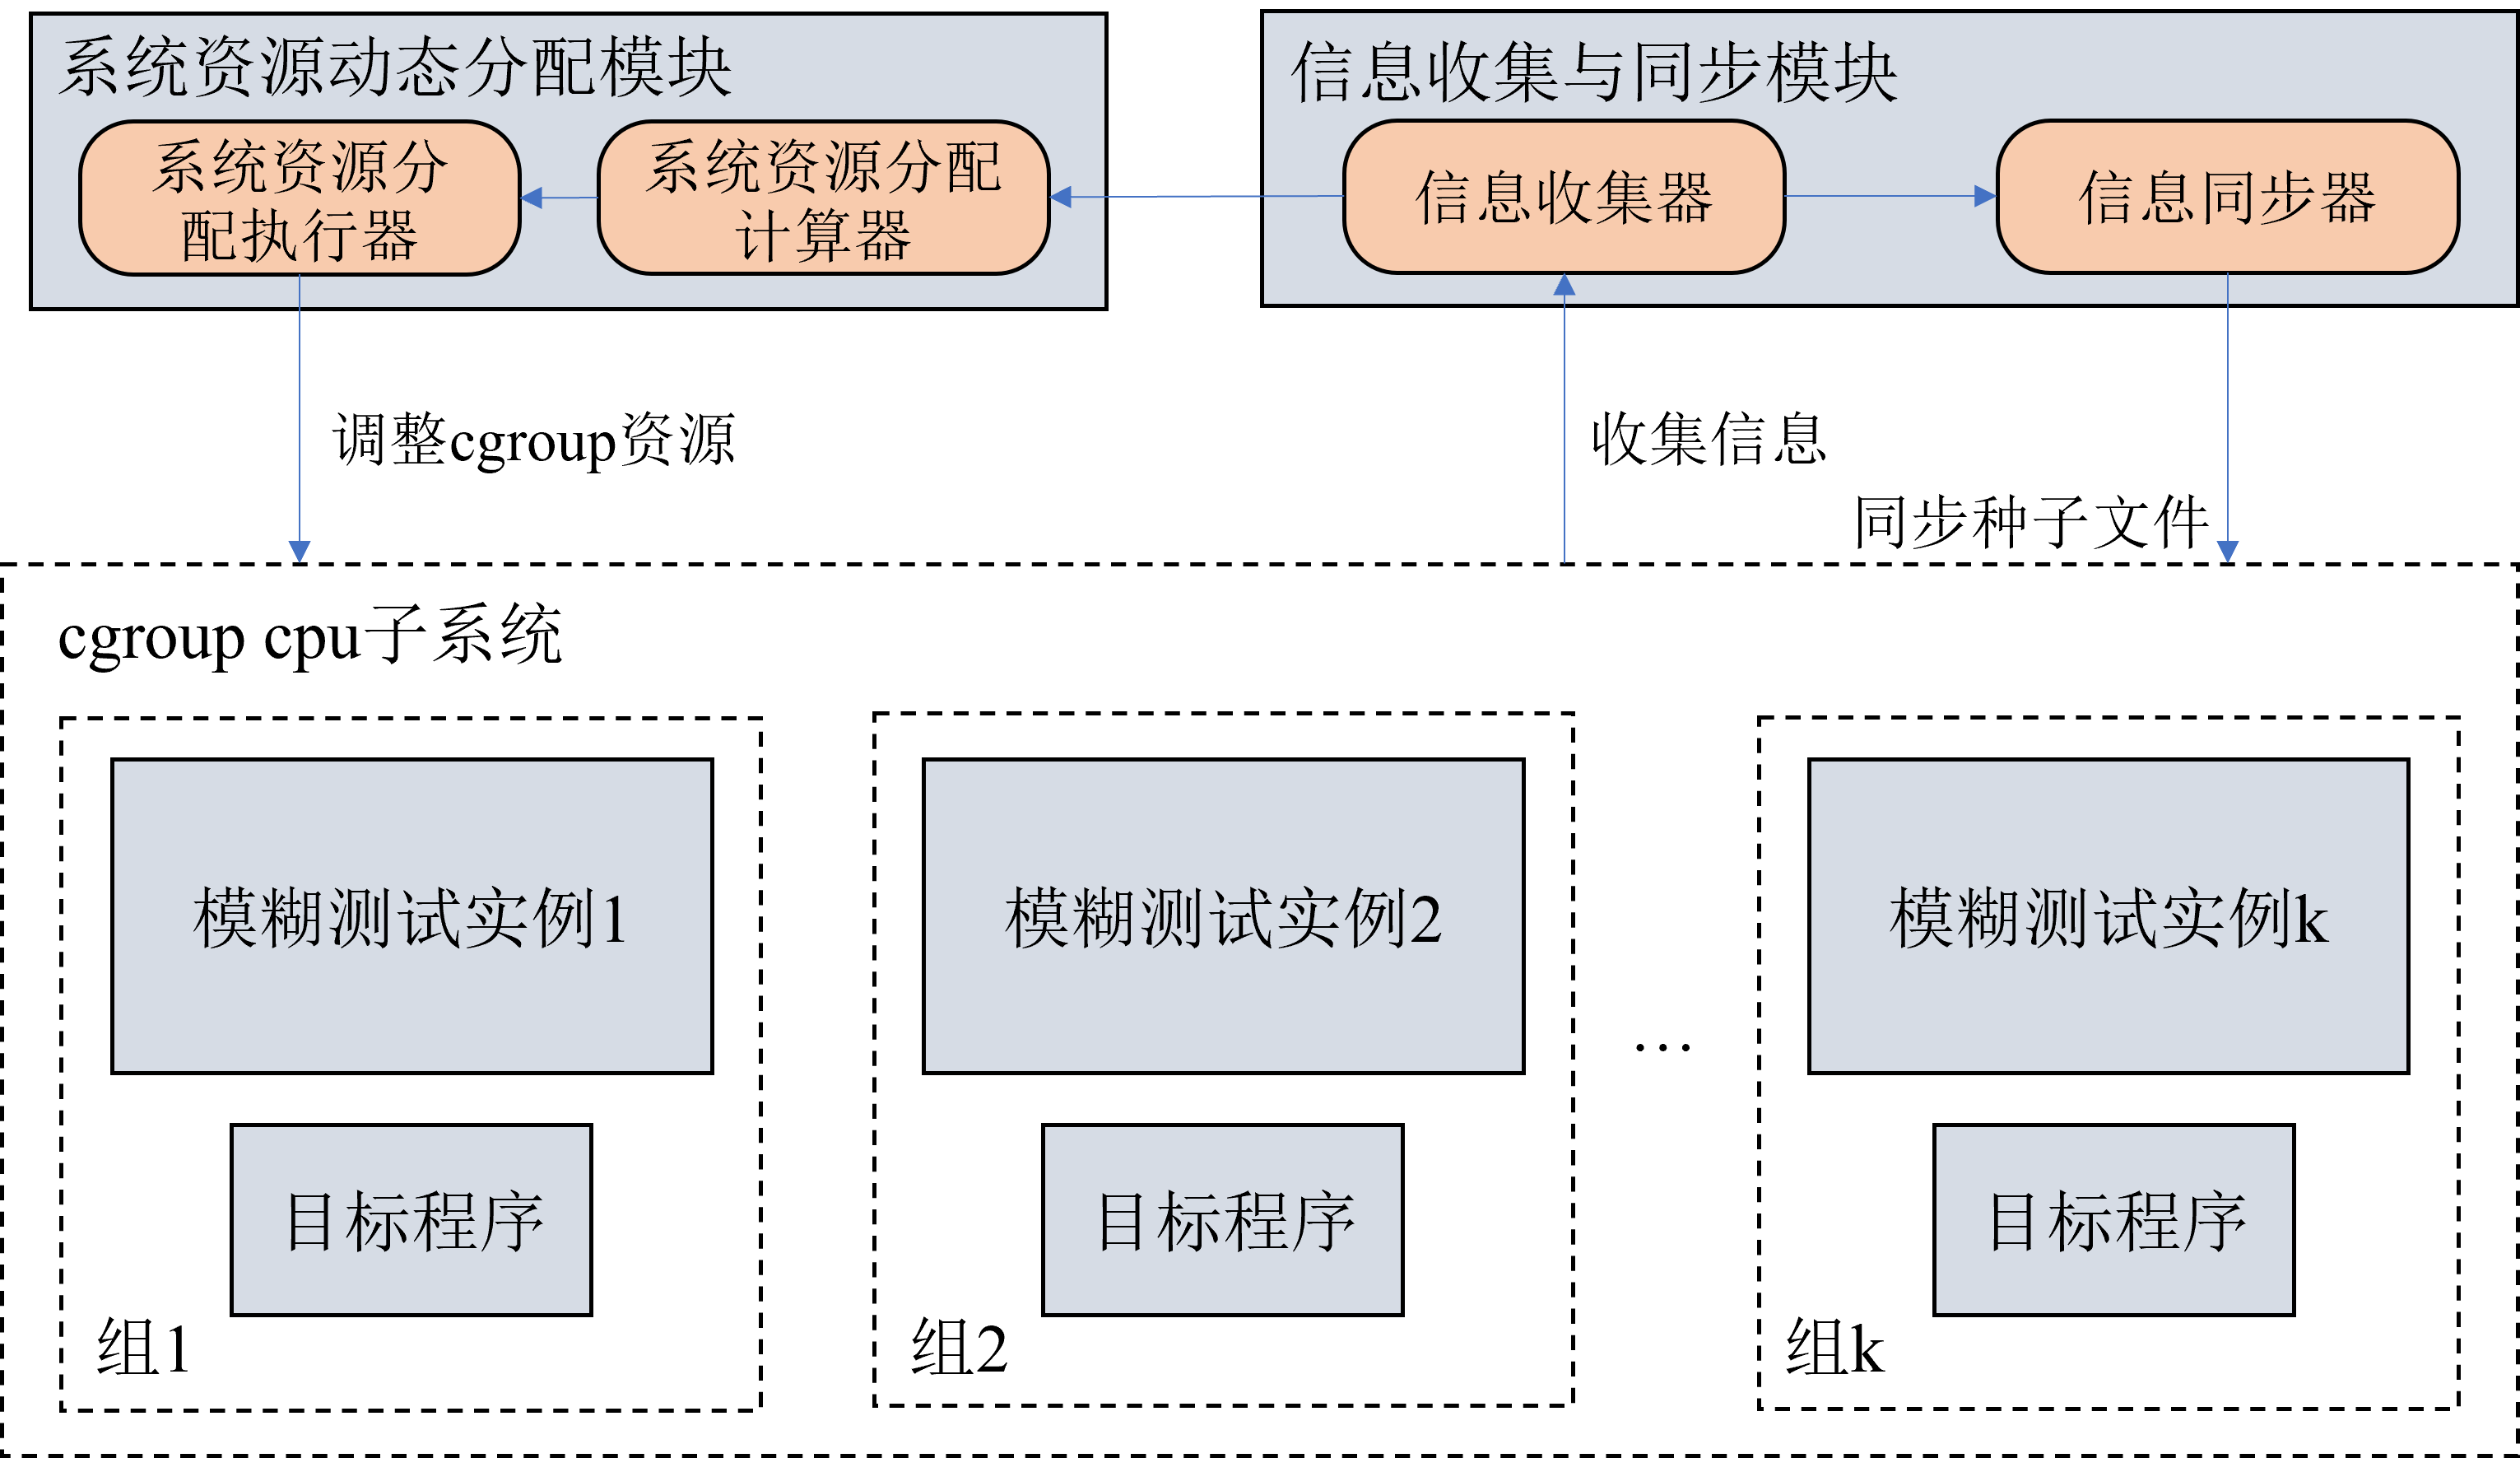
\includegraphics[width=14cm]{cgroup.png}
    \caption{系统资源动态分配子系统架构}
    \label{cgroup}
\end{figure}

\section{跨实例种子调度技术}
已有的异构并行模糊测试工具并不具备跨实例种子调度的能力,工具对各模糊测试实例的管理能力较弱,影响了并行模糊测试效率的进一步提升。为了解决这一问题,本节将从种子效率研究和种子调度算法设计与实现两个部分,介绍本文系统使用的跨实例种子调度技术。
\subsection{种子效率研究}
% 已有种子调度策略分析
% 观察得到种子执行数与频率的关系

在模糊测试中,种子的执行次数会影响测试的覆盖率和深度。通常情况下,对于一个种子,如果它在尽可能短的时间内执行的次数越多,就越有可能发现一些深度更深、覆盖面更广的漏洞,因为它已经深入了目标程序的不同部分,并产生了更广泛的输入。因此,在实践中,通常会尽可能多地执行每个种子,以最大化测试的覆盖率和深度。

然而尽可能多的执行每个种子会受到现实因素的限制,因为模糊测试通常有时间上的要求,希望在有限时间发现更多的漏洞,因此对每个种子进行全面的测试是不现实的。

对于一个种子来说,它被执行的次数越多,通过它得到新种子的可能性就越小。这是因为模糊测试的目的是尽可能发现新的漏洞,而已经被多次执行的种子已经被充分测试过,可能已经生成了其他新的种子,则不太可能发现新的路径或漏洞。因此,在实践中,为了提高模糊测试的效率,通常会使用某些技术,例如基于覆盖率指导的种子挑选技术,优先对尚未充分测试的种子进行进一步测试,从而提高发现新种子的效率。

文献\cite{wang2021facilitating}对AFL的并行模式进行了研究。在四个流行的基准测试程序(objdump、readelf、libxml、nm)上使用 2 个并行实例运行 AFL 24 小时。跟踪变异过程以了解哪些种子由哪些实例变异。结果表明,尽管许多种子从未发生变异,但不同的实例确实存在变异重叠的种子。以 6 小时后的结果为例,平均而言,近 20\% 的种子从未发生变异。然而,超过 42\% 的种子接受了多轮变异。文献\cite{wang2021facilitating}还观察到一种趋势,即变异种子之间的重叠越少,代码覆盖率就越高。文献\cite{wang2021facilitating}的实证研究表明,AFL(可能还有许多其他模糊测试工具)的并行模式确实会带来重叠,这进一步阻碍了代码覆盖的效率。

\begin{table}[!htbp]
    \caption{模糊测试工具种子调度策略}
    \begin{tabular}{ll}
    \toprule
    模糊测试工具 & 种子调度策略 \\
    \midrule
    AFLFast & 低频路径优先 \\
    Fairfuzz & 稀缺分支优先 \\
    Collafl &  未触及的邻居分支多优先 \\
    Tortoisefuzz & 更多危险操作优先 \\
    Savior & 未触及邻居分支的危险操作多优先 \\
    \bottomrule
    \end{tabular}
    \label{table_seeds}
    \vspace{6pt}
\end{table}

对于异构并行模糊测试来说,这个问题同样存在。尽管不同的模糊测试实例使用不同的种子挑选策略,但是不同策略下的种子集合仍然会有重叠,图\ref{celue}是一个简单的示例。特别来说,部分模糊测试种子挑选算法较为相近,如AFLFast和Fairfuzz的策略都倾向于选择低频分支的种子、Savior和Collafl都倾向于选择未触及的邻居多的种子,在这种情况下,种子集重叠的范围会更大。那些处于重叠范围内的种子会获得比其余种子更多的执行次数,随着模糊测试的进行,花费时间在这些种子上的性价比将不断变低。

\begin{figure}[!htbp]
    \vspace{6pt}
    \centering
    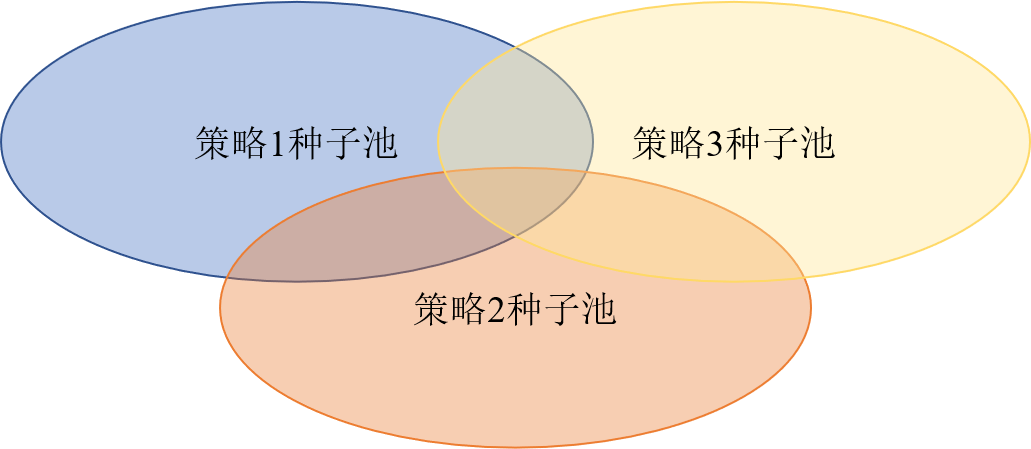
\includegraphics[width=12cm]{cross.png}
    \caption{不同策略种子池}
    \label{celue}
\end{figure}


为了确认种子集重叠问题的存在和其影响,本文收集并统计了异构并行模糊测试中,不同种子的执行次数和每次选择种子后发现新种子的效率(发现新种子的数量/执行次数)。为了便于数据的统计,需要根据种子的执行次数,将其动态分成$k$组。具体步骤如下:

1)首先将种子按照其执行次数从小到大的顺序进行排序。

2)然后从第一个种子开始,依次将每个种子加入当前的分组,直到该分组的数值之和大于等于总和的$1/k$,其中$k$为需要分成的组数。

3)如果当前分组的数值之和已经接近总和的$1/k$,或者已经处理完了所有种子,则将当前分组存储起来,并开始处理下一个分组。

4)重复步骤2和3,直到所有种子都被分组完毕。

这种贪心算法的时间复杂度为$O(nlogn)$,其中$n$为种子的个数。是一种时间复杂度较低的分类算法,能够在较短时间内将种子集合根据其执行次数的关系进行分类,执行次数相近的种子将被分在同一个类中,并且每个分类中种子的执行数量的总和基本相等。

在本小节的验证实验中,$k$取5,即将种子根据执行次数分成5组,种子的分组情况是动态更新的。实验被测试的软件为as、nm、objdump和readelf,并行的模糊测试实例为AFL、Fairfuzz、Mopt、Tortoisefuzz、Angora和QSYM,测试时长为12小时,实验结果重复5次取平均值。

图\ref{fenbu}展示了不同分组种子被执行的次数占总执行次数的比例,as测试中不同分组占比为76.20\%、14.40\%、7.44\%、1.78\%、0.18\%;nm测试中不同分组占比为22.62\%、21.40\%、20.57\%、19.40\%、16.01\%;objdump测试中不同分组占比为56.78\%、14.76\%、11.55\%、8.66\%、8.25\%;readelf测试中不同分组占比为61.32\%、12.55\%、10.24\%、9.19\%、6.70\%。

对于测试的四款软件、其属于最高执行次数分组的种子的执行次数仍然占据一定比例,平均占比达到了7.79\%,反映了在异构并行模糊测试中,仍然存在一定程度的种子重叠问题。

% 提出跨实例种子调度算法

\begin{figure}[t]
    \vspace{6pt}
    \centering
    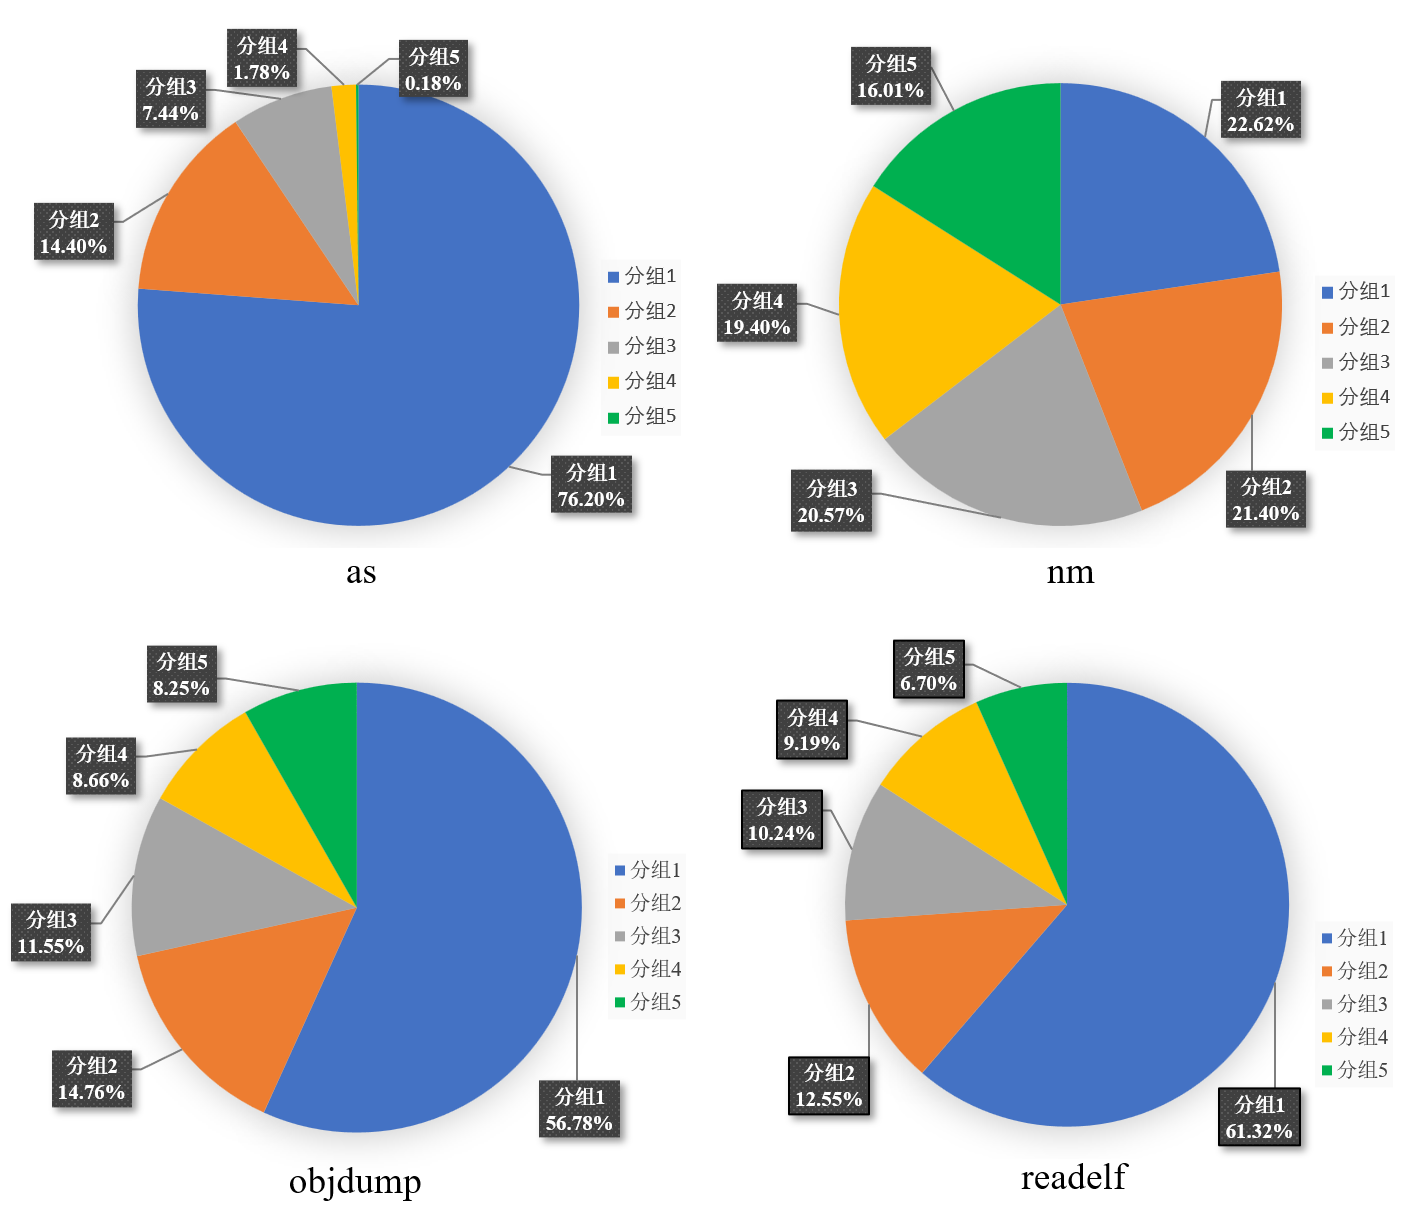
\includegraphics[width=15cm]{pie.png}
    \caption{种子执行次数分布}
    \label{fenbu}
\end{figure}

表\ref{table_eff}展示了不同分组种子被执行生成新种子的效率与测试平均效率的差异,as测试中不同分组的测试效率与测试平均效率的差异为+20.3\%、-56.2\%、-67.4\%、-70.6\%、-76.4\%;nm测试中不同分组的测试效率与测试平均效率的差异为+205.8\%、-74.2\%、-87.7\%、-89.0\%、-93.7\%;objdump测试中不同分组的测试效率与测试平均效率的差异为+35.1\%、-73.3\%、-75.9\%、-85.5\%、-91.3\%;readelf测试中不同分组的测试效率与测试平均效率的差异为+44.3\%、-68.9\%、-72.9\%、-84.1\%、-93.1\%。根据表中的数据可以发现,对于所有被测试的软件,其种子执行次数最低的分组中的种子的执行效率都要高于平均的执行效率,随着执行次数的增加,各个分组中种子的执行效率将不断降低。

\begin{table}[!htbp]
    \caption{种子执行次数与平均效率的关系}
    \begin{tabular}{llllll}
    \toprule
    测试程序 & 分组1 & 分组2 & 分组3 & 分组4 & 分组5 \\
    \midrule
    as & +20.3\% & -56.2\% & -67.4\% & -70.6\% & -76.4\%  \\
    nm & +205.8\% &- 74.2\% & -87.7\% & -89.0\% & -93.7\%    \\
    objdump & +35.1\% & -73.3\% & -75.9\% & -85.5\% & -91.3\% \\
    readelf & +44.3\% & -68.9\% & -72.9\% & -84.1\% & -93.1\% \\
    \bottomrule
    \end{tabular}
    \label{table_eff}
    \vspace{6pt}
\end{table}

通过上述数据可以发现,对于被测试的四款软件,它们测试过程中处于第一个分组(执行次数最低)中的种子的平均测试效率高于所有种子的平均测试效率,而其他分组中种子的平均测试效率低于所有种子的平均测试效率,并且平均执行次数更高的分组中的种子的效率会更低。充分验证了在异构并行模糊测试中,也存在种子集重叠的问题,并且这个问题会导致总体测试效率的降低。

% 在模糊测试中,一个种子被执行的次数与它能够发现新代码覆盖的测试用例数目之间存在着一定的关系。可以使用测试用例执行次数的期望值和测试用例生成新样本的期望值来衡量这种关系。

% 设一个种子被执行的次数为 $N$,发现的新代码覆盖测试用例数为 $M$,则其测试用例执行次数的期望值为 $E(N)$,测试用例生成新样本的期望值为 $E(M)$。

% 在模糊测试中,为了尽可能发现更多的新代码覆盖,一般会增加每个种子的执行次数。但是,增加执行次数也会导致测试时间和资源消耗增加。因此,需要在执行次数和发现新样本数之间寻找一个平衡点。

% 通常,可以通过实验得到种子被执行次数和发现新样本数之间的关系,然后使用数学方法拟合出一条曲线。根据这条曲线,可以预测执行某个种子 $N$ 次后可以发现多少个新样本。同时,也可以预测在发现一定数量的新样本后,需要执行多少次测试用例才能发现更多的新样本。

% 需要注意的是,由于测试用例生成算法和被测试程序的复杂度不同,不同的模糊测试工具在同一种子上的测试结果可能会不同。因此,这种预测方法只是一种参考,具体的测试结果仍需要通过实验来验证。

\subsection{种子调度算法设计与实现}

本小节将在上一小节得到的种子已执行次数与种子探索效率关系的基础上,提出跨实例种子调度算法,并给出工程上的实现方式。

异构并行模糊测试中产生种子集重叠问题的原因是各模糊测试实例虽然同步了种子信息,但是仅限于同步种子的原始数据。种子同步后,各模糊测试实例并不知道该种子在其他模糊测试实例中的执行情况,即使当前实例的种子选择策略考虑了种子的执行次数,但是也仅限在本实例中的执行次数。假设一个种子在其他模糊测试实例中得到了充分的测试,但当前模糊测试实例对其完全不知情,仍可能选中该种子对其进行大量的测试。这些测试的效率很可能会十分低下,影响整体并行模糊测试的效率,因此要通过算法来降低此类情况出现的概率。

4.1.2小节给出了并行模糊测试的优化算法,算法\ref{parallel_fuzzing_pro}展示了在一次模糊测试迭代中,模糊测试实例会依次经过同步信息、种子调度、用例生成、测试用例评估等过程。为了保证本小节算法的通用性,应该将跨实例种子调度这一过程应该在不破坏原有模糊测试流程的基础上,作为一个独立的环节嵌入迭代的串行过程中。本系统将跨实例种子调度环节加入到种子调度环节之后,用例生成环节之前。这样的设计保证了原有模糊测试实例仍能按照自身的逻辑进行模糊测试。

该算法涉及到三个具体实例,其一是模糊测试实例,它负责执行具体的模糊测试任务;其二是全局种子数据库,该数据库维护每个种子的有效信息,包括种子id、执行次数、执行发现的新种子数量和潜在效率,其中潜在效率代表该种子未来发现新种子的能力;其三是全局种子调度器,它通过分析已有数据推算出每个种子的潜在效率。

具体跨实例种子调度的流程如图\ref{seeds_process}所示。数据库首先进行初始化,所有已发现的种子的潜在效率都为最高。在一次模糊测试迭代中,模糊测试实例在进行种子调度后已选出当前的原始种子并计算好种子所分配的能量,然后访问全局种子数据库,获取当前种子的潜在效率,根据潜在效率具体的数值决定是否跳过用例生成和测试用例评估阶段。然后模糊测试实例将当前迭代种子的测试结果(执行次数、新发现的种子数)上传到全局种子数据库中进行更新。全局种子调度器将通过最新的种子测试情况更新种子的潜在效率。

\begin{figure}[!htbp]
    \vspace{6pt}
    \centering
    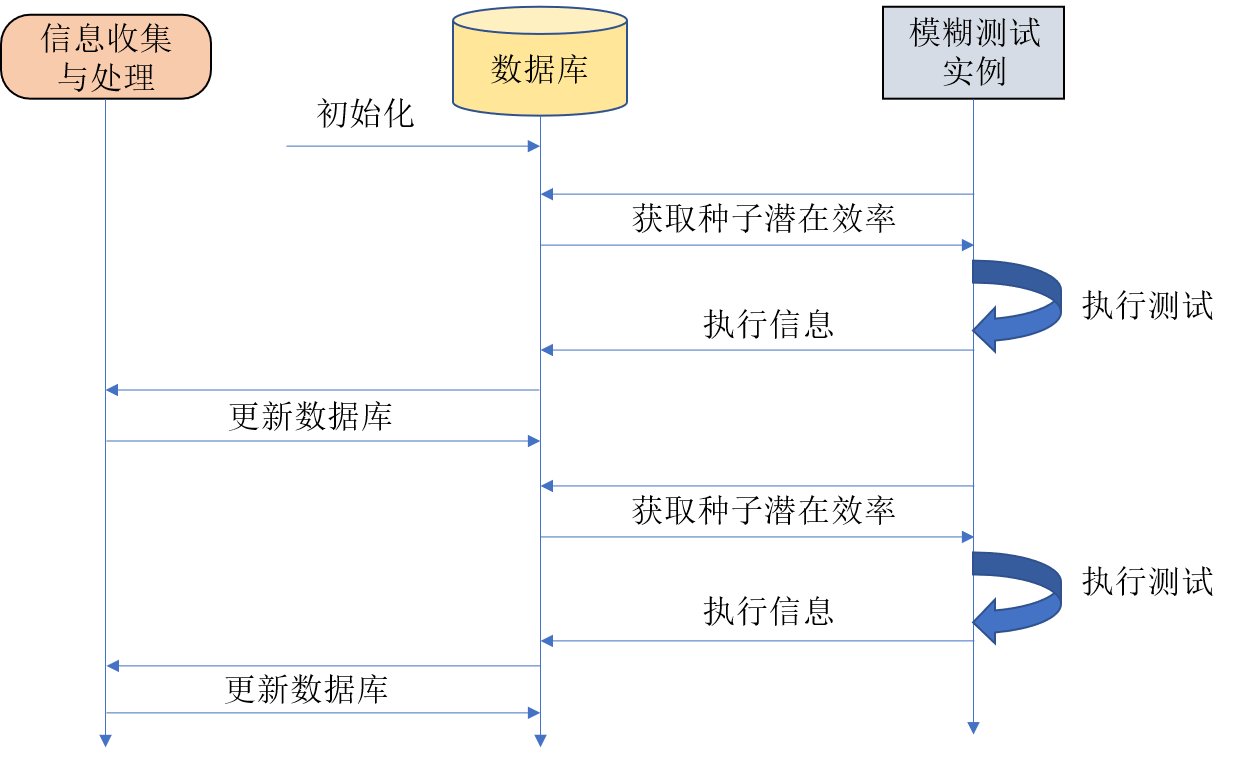
\includegraphics[width=15cm]{seeds_process.png}
    \caption{跨实例种子调度流程图}
    \label{seeds_process}
\end{figure}

对于模糊测试实例来说,为了使得扩展难度降低,具体工程实现上应该尽可能简单。本文将种子潜在效率这一数值范围限定在八位无符号整型(0-255)范围内,当模糊测试实例获取到该值后,自身再通过随机的方法产生一个0-255范围内的随机数,如果生成的随机数大于种子潜在效率的值,则跳过用例生成和用例测试评估阶段。可以发现,如果种子潜在效率始终为255,无论如何模糊测试实例都不会跳过这两个阶段,和已有的模糊测试逻辑完全相同。
\begin{equation}
    f_{score}(\bm{x})=
    \begin{cases}
    \min\{255, \left\lfloor  255 * \frac{e_1}{e_{avg}} \right\rfloor\} & \bm{x} \in \mathbb{G}_1 \\
    \min\{255, \left\lfloor  255 * \frac{e_2}{e_{avg}} \right\rfloor\} & \bm{x} \in \mathbb{G}_2 \\
    \min\{255, \left\lfloor  255 * \frac{e_3}{e_{avg}} \right\rfloor\} & \bm{x} \in \mathbb{G}_3 \\
    \min\{255, \left\lfloor  255 * \frac{e_4}{e_{avg}} \right\rfloor\} & \bm{x} \in \mathbb{G}_4 \\
    \min\{255, \left\lfloor  255 * \frac{e_5}{e_{avg}} \right\rfloor\} & \bm{x} \in \mathbb{G}_5 
    \end{cases}
    \label{cross}
\end{equation}

最重要的部分为种子潜在效率数值的确定,为了避免执行次数过高的种子对整体测试效率的影响,应该尽可能降低选中这类种子的概率。但是考虑到不同模糊测试实例生成测试用例的技术不同,即使其他模糊测试实例对某个种子进行了较为全面的测试,当前模糊测试实例也有可能因为其生成测试用例的特殊性,通过该种子生成新的种子。因此应当保留一定的概率使得执行次数过高的种子仍有可能被选择并执行。本文提出的种子潜在效率数值的计算公式如公式\ref{cross}所示,根据种子的执行次数确认种子所在的分组,种子的潜在效率为最大潜在效率255乘以当前分组效率$e_{i}$($i$为当前分组号)与整体平均效率$e_{avg}$的比值,种子的潜在效率最大不超过255。


\section{本章小结}

本章首先介绍了信息收集与同步技术,包括信息收集器与信息同步器的实现原理;然后介绍了系统资源动态调度技术,分析得出并行模糊测试需要动态分配的系统资源类型,并重点介绍预测模糊测试实例效率的方法与整体的系统资源动态分配算法的设计与实现;最后介绍了跨实例种子调度技术,通过分析种子执行次数与种子效率的关系,得到了种子效率与种子执行次数负相关的结论,并以此设计并实现跨实例种子调度模块。 

\chapter{动态策略并行模糊测试系统验证实验}

本章首先介绍动态策略并行模糊测试系统验证实验的实验环境、选取的被测试软件和选取的模糊测试实例,然后对测试系统在细粒度信息收集、系统资源动态分配、跨实例种子调度和提升测试效率上的能力进行验证,并对验证结果进行展示和分析。

\section{测试准备}
\subsection{实验环境}

本文动态策略并行模糊测试系统验证实验使用的服务器,其配置信息如表\ref{table_server}所示。为充分利用服务器资源,在有限时间内进行多次实验,本文使用KVM\citing{kivity2007kvm}虚拟化技术在服务器上创建多个KVM虚拟机,虚拟机配置如表\ref{table_kvm}所示。所有的实验测试均于KVM虚拟机中进行。

\begin{table}[!htbp]
    \caption{服务器配置信息表}
    \begin{tabular}{lllll}
    \toprule
    服务器型号 & CPU型号 & CPU核心数 & 内存大小 & 磁盘大小 \\
    \midrule
    \makecell[l]{戴尔机架式服务器 \\ Dell PowerEdge R740 }
 & \makecell[l]{Intel(R) Xeon(R) CPU \\ Gold 6230R @ 2.10GHz} & 52核 & 256GB & 20TB \\
    \bottomrule
    \end{tabular}
    \label{table_server}
    \vspace{6pt}
\end{table}

\begin{table}[!htbp]
    \caption{虚拟机配置信息表}
    \begin{tabular}{llll}
    \toprule
    操作系统 & 虚拟CPU个数 & 虚拟内存大小 & 虚拟磁盘大小 \\
    \midrule
    Ubuntu16.04 & 4核 & 8GB & 50GB \\
    \bottomrule
    \end{tabular}
    \label{table_kvm}
    \vspace{6pt}
\end{table}
% 实验软件环境
% \begin{table}[!htbp]
%     \caption{实验软件环境}
%     \begin{tabular}{cccc}
%     \toprule
%     软件 & 版本 \\
%     \midrule
%     ubuntu & 16.04 \\
%     python & 2.12 \\
%     clang & 10\\
%     gcovr &  未触及的邻居分支多优先 \\
%     \bottomrule
%     \end{tabular}
%     \label{table_soft}
%     \vspace{6pt}
%\end{table}

\subsection{被测试软件选取}

Binutils\citing{ref_binutils}是一组用于操作二进制文件的开源工具,广泛应用于操作系统、编译器、调试器等软件的开发中。选择Binutils作为模糊测试的对象有以下几个原因:1)Binutils是一个非常复杂的软件包,由多个程序组成,涉及到多种操作和数据类型,因此它很可能存在多种漏洞;2)Binutils被广泛使用,存在于大量的软件和系统中,因此发现和修复Binutils中的漏洞可以带来广泛的安全性和稳定性影响;3)Binutils的代码是公开的,易于获取和分析,测试人员可以根据需要对其进行修改和扩展,从而提高模糊测试的效率和效果;4)在实际应用中,模糊测试常常用于发现新的漏洞,而Binutils的开发者已经投入了大量的资源来保证其质量,因此它在一定程度上可以作为一种标准的测试对象,可以帮助测试人员更准确地评估模糊测试的效果。

本文实验具体选取Binutils-2.28中的as、nm、objdump和readelf软件作为被测试对象,具体运行这些软件的参数如表\ref{table_targets}所示。

\begin{table}[!htbp]
    \caption{被测试软件介绍}
    \begin{tabular}{lll}
    \toprule
    软件名 & 软件功能 & 测试参数 \\
    \midrule
    as & 将汇编文件转化为对象文件 & -o /dev/null \\
    nm & 列出给定对象文件中出现的符号 & \makecell[l]{-A -a -l -S -s --special-syms \\--synthetic --with-symbol-versions -D}  \\
    objdump & 查看对象文件信息 & -S \\
    readelf & 查看elf文件 & -a \\
    \bottomrule
    \end{tabular}
    \label{table_targets}
    \vspace{6pt}
\end{table}

% todo 初始种子

\subsection{模糊测试实例选取}

本文实验具体选取AFL、Mopt、Fairfuzz、Tortoifuzz、Angora和QSYM工具作为动态策略并行模糊测试系统中的模糊测试实例,每种实例各一个。AFL是当前最流行的模糊测试工具之一,其余五款工具均发表于高水平会议中。在具体运行这些实例的部分参数如表\ref{table_instances}所示。

% todo
\begin{table}[!htbp]
    \caption{选取的模糊测试实例}
    \begin{tabular}{lll}
    \toprule
    工具 & 工具特点 & 测试配置 \\
    \midrule
    AFL & 执行速度快 & -S afl \\
    Mopt & 动态调整变异算子选择概率 & -L 1 -S mopt \\
    Fairfuzz & 针对稀缺分支进行测试 & -q 1 -S fairfuzz \\
    Tortoisefuzz & 针对危险代码段进行测试 & -S tf -s \\
    Angora & 使用污点分析技术生成测试用例 & -S \\
    QSYM & 使用符号执行技术生成测试用例 & -a afl -n qsym \\
    \bottomrule
    \end{tabular}
    \label{table_instances}
    \vspace{6pt}
\end{table}

\section{细粒度信息收集能力验证实验}
本节将通过实验验证动态策略并行模糊测试系统的细粒度信息收集能力,具体包括种子执行情况收集能力和模糊测试效率信息收集能力。
\subsection{种子执行情况收集能力验证}

种子执行情况指的是不同模糊测试实例对种子的执行次数和发现新种子的数量,可以为后续动态策略的实施提供参考。通过对模糊测试实例代码加入少量探针代码,可以实时记录每个模糊测试实例的种子执行情况,具体输出的执行情况如图\ref{exec_log}所示。可以发现,不同的模糊测试实例在执行完一次种子测试的迭代后,会依次打印实例id、执行的种子路径、执行次数和发现新种子的数量。

\begin{figure}[!htbp]
    \vspace{6pt}
    \centering
    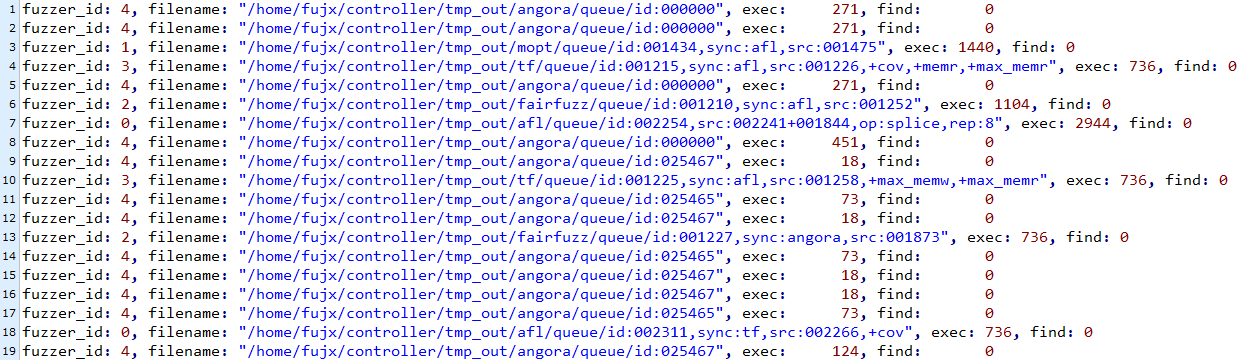
\includegraphics[width=15cm]{exec_log.png}
    \caption{模糊测试实例种子执行情况}
    \label{exec_log}
\end{figure}

每一条记录能够说明当前种子实时测试效率的情况,然而由于同步机制的存在,相同的种子可能存在于不同模糊测试实例的种子队列中,文件名也不相同,需要对相同的种子的执行情况进行合并。系统因此使用文件的MD5哈希值作为区分种子的标识。如图\ref{watch_dog}所示,系统在检测到目标文件夹产生了新的文件后,会计算其MD5值。文件名和其MD5的映射关系会保存作为对种子执行情况去重的依据。

\begin{figure}[!htbp]
    \vspace{6pt}
    \centering
    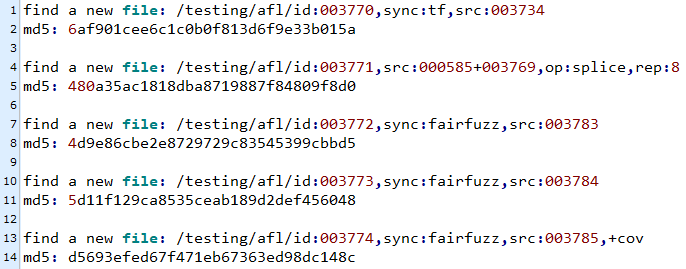
\includegraphics[width=15cm]{watchdog.png}
    \caption{文件名MD5映射表}
    \label{watch_dog}
\end{figure}

图\ref{uniq_exec}展示了去重之后的种子执行情况,第一列为种子的MD5值,第二列为种子的总执行次数,该信息能够用于根据执行次数的高低给种子分组。

\begin{figure}[!htbp]
    \vspace{6pt}
    \centering
    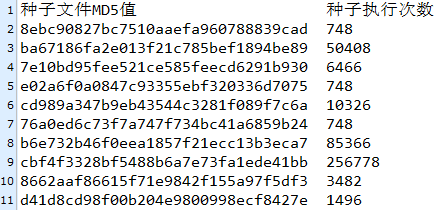
\includegraphics[width=10.5cm]{uniq_exec.png}
    \caption{种子去重后执行次数}
    \label{uniq_exec}
\end{figure}

\subsection{模糊测试效率信息收集能力验证}

通过处理图\ref{uniq_exec}所示的信息,即可以对种子依据执行次数进行排序分组,如图\ref{run_log}的3-6行,系统计算出了第2组到第5组的门限值。根据门限值和5.2.1小节的数据,可以统计上一个时间段内,不同分组下的种子的执行次数与发现新种子的数量,进而计算出各分组的测试效率。图\ref{kv}展示了种子的预测效率情况,其中第一列为种子的MD5哈希值,第二列为种子的潜在测试效率。种子潜在效率的数值能够间接指导模糊测试实例选择更有价值的种子。

\begin{figure}[!htbp]
    \vspace{6pt}
    \centering
    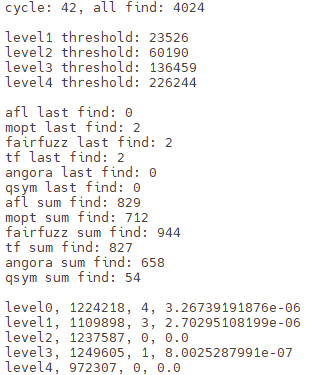
\includegraphics[width=8.5cm]{run_log.png}
    \caption{系统运行日志}
    \label{run_log}
\end{figure}

\begin{figure}[!htbp]
    \vspace{6pt}
    \centering
    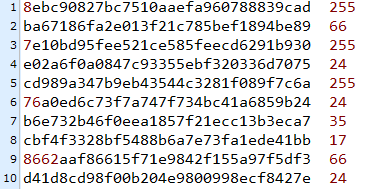
\includegraphics[width=10.5cm]{kv-eff.png}
    \caption{种子效率数据库}
    \label{kv}
\end{figure}

除此之外,系统还收集了一定时间段内各模糊测试实例的种子发现情况,该统计方法不是使用模糊测试实例自行打印的日志信息,因为在一个时间范围内,不同模糊测试实例对发现新种子可能存在重复,因此使用全局的种子路径分析来确定种子发现情况。如图\ref{run_log}的8-13行,工具输出了每个模糊测试实例的种子发现数量。该数据是指导系统资源动态分配模块的必要输入。

\section{系统资源动态分配能力验证实验}

上一节展示了本文设计的系统对各模糊实例测试情况的收集能力,本节将验证本系统的系统资源动态分配能力。为了直观地展示动态分配资源的有效性,实验收集了不使用系统资源动态分配策略与使用系统资源动态分配策略这两种情况下各模糊测试实例的总执行次数。表\ref{table_alloc}展示了对不同软件进行测试时,测试效果最好的模糊测试实例和它在资源分配前后的执行次数。AFL对as的测试效果最好,资源分配后执行次数提高了4.2\%,Tortoisefuzz对nm的测试效果最好,资源分配后执行次数提高了2.6\%,Fairfuzz对objdump和readelf的测试效果最好,资源分配后执行次数分别提高了11.2\%和5.1\%。由表中数据可以得出结论,本系统的系统资源动态分配模块能够有效地提高测试效果好的模糊测试实例的执行次数。

\begin{table}[!htbp]
    \caption{模糊测试实例执行情况}
    \begin{tabular}{lllll}
    \toprule
    软件 & 测试效果最好的实例 & 原始执行次数 & 资源分配后执行次数 & 执行次数变化 \\
    \midrule
    as & AFL & 5310944 & 5531604 & +4.2\% \\
    nm & Tortoisefuzz & 26727003 & 27430418 & +2.6\% \\
    objdump & Fairfuzz & 14209630 & 15806944 & +11.2\% \\
    readelf & Fairfuzz & 26695239 & 28059036 & +5.1\% \\
    \bottomrule
    \end{tabular}
    \label{table_alloc}
    \vspace{6pt}
\end{table}

\section{跨实例种子调度能力验证实验}
本节将验证跨实例种子调度的有效性。为了直观的展示跨实例种子调度策略的效果,本文对于四款软件(as、nm、objdump和readelf)进行测试,收集不使用跨实例种子调度策略与使用跨实例种子调度策略这两种情况下并行模糊测试每个种子的执行次数,将种子按照执行次数分入对应的分组($[0, 2000)$、$[2000, 4000)$、$[4000, 6000)$、$[6000, 8000)$、$[8000, 10000)$和$[10000, \infty)$)中,再统计每个分组中种子数量与总种子数量的占比。表\ref{table_ss}展示了具体的分组占比情况。通过表中的数据可以发现,对于四款被测试的软件,使用跨实例种子调度策略后,执行次数较高的分组占比降低,而执行次数较低的分组占比有所提升。因此能够得出结论,跨实例种子调度策略能够让模糊测试实例偏向于选择并执行较低执行次数的种子,降低了种子被过度执行的概率。
\begin{table}[!htbp]
    \caption{种子执行次数分布}
    \begin{tabular}{lllll}
    \toprule
    软件 & 执行次数范围 & 原始策略 & 跨实例种子调度 & 变化\\
    \midrule
    \multirow{6}{30pt}{as} & $[0, 2000)$ & 71.4\% & 73.5\% & +2.1\%   \\
    & $[2000, 4000)$ & 18.1\% & 17.3\% & -0.8\%  \\
    & $[4000, 6000)$ & 4.9\% & 4.2\% & -0.7\%  \\
    & $[6000, 8000)$ & 2.6\% & 2.1\% & -0.5\%\\
    & $[8000, 10000)$ & 2.4\% & 2.4\% & 0\%  \\
    & $[10000, \infty)$ & 0.6\% & 0.5\% & -0.1\% \\
    \specialrule{0.05em}{3pt}{3pt} 
    \multirow{6}{30pt}{nm} & $[0, 2000)$ & 49.1\% & 52.7\% & +3.6\%   \\
    & $[2000, 4000)$ & 9.6\% & 11.4\% & +1.8\%  \\
    & $[4000, 6000)$ & 5.1\% & 6.4\% & +1.3\%  \\
    & $[6000, 8000)$ & 3.2\% & 4.2\% & +1.0\%\\
    & $[8000, 10000)$ & 3.4\% & 4.0\% & +0.6\%  \\
    & $[10000, \infty)$ & 29.6\% & 21.3\% & -8.3\% \\
    \specialrule{0.05em}{3pt}{3pt} 
    \multirow{6}{50pt}{objdump} & $[0, 2000)$ & 33.8\% & 34.9\% & +1.1\%   \\
    & $[2000, 4000)$ & 21.9\% & 22.8\% & +0.9\%  \\
    & $[4000, 6000)$ & 13.9\% & 14.9\% & -1.0\%  \\
    & $[6000, 8000)$ & 8.8\% & 7.5\% & -1.3\%\\
    & $[8000, 10000)$ & 5.8\% & 5.4\% & -0.4\%  \\
    & $[10000, \infty)$ & 15.8\% & 14.5\% & -1.3\% \\
    \specialrule{0.05em}{3pt}{3pt} 
    \multirow{6}{30pt}{readelf} & $[0, 2000)$ & 46.7\% & 48.5\% & +1.8\%   \\
    & $[2000, 4000)$ & 29.4\% & 31.0\% & +1.6\%  \\
    & $[4000, 6000)$ & 11.9\% & 11.0\% & -0.9\%  \\
    & $[6000, 8000)$ & 4.5\% & 4.4\% & -0.1\%\\
    & $[8000, 10000)$ & 2.7\% & 2.6\% & -0.1\%  \\
    & $[10000, \infty)$ & 4.8\% & 2.5\% & -2.3\% \\
    \bottomrule
    \end{tabular}
    \label{table_ss}
    \vspace{6pt}
\end{table}

\section{测试效率提升验证实验}

本节将通过对目标程序真实的测试来体现动态策略并行模糊测试系统中两大动态策略功能对测试性能的影响。由于本系统的两种动态策略的实施并不会相互干扰,因此实验将比较原始并行策略(Collabfuzz)、系统资源动态分配策略(DSPFuzzer-RA)、跨实例种子调度策略(DSPFuzzer-SS)和两种策略相结合的策略(DSPFuzzer-FULL),分析它们在代码覆盖和崩溃发现数量上的性能差异。为了尽可能消除实验误差,每种类型的测试都将测试12小时,并且重复10次取测试结果的平均值。

\subsection{代码覆盖提升验证}

为了更准确的评估代码覆盖性能,本小节将采用三种代码覆盖的评估指标对实验结果进行分析,分别为行覆盖、分支覆盖和路径覆盖。

% 其中行覆盖和分支覆盖使用gcov工具进行插桩,需要在编译程序时添加"-fprofile-arcs"和"-ftest-coverage"选项。在实验结束后,按种子文件发现的时间顺序依次重新运行插桩后的程序,并在程序源码的主文件夹使用“gcovr -r . -s | grep "[lb][a-z]*:"”命令收集具体的行覆盖和分支覆盖信息。

% 路径覆盖使用AFL工具提供的分析方法,如果当前种子文件存在新执行的边信息时,则认为发现了一条新的路径。

(1)行覆盖

\begin{figure}[!htbp]
    \vspace{6pt}
    \centering
    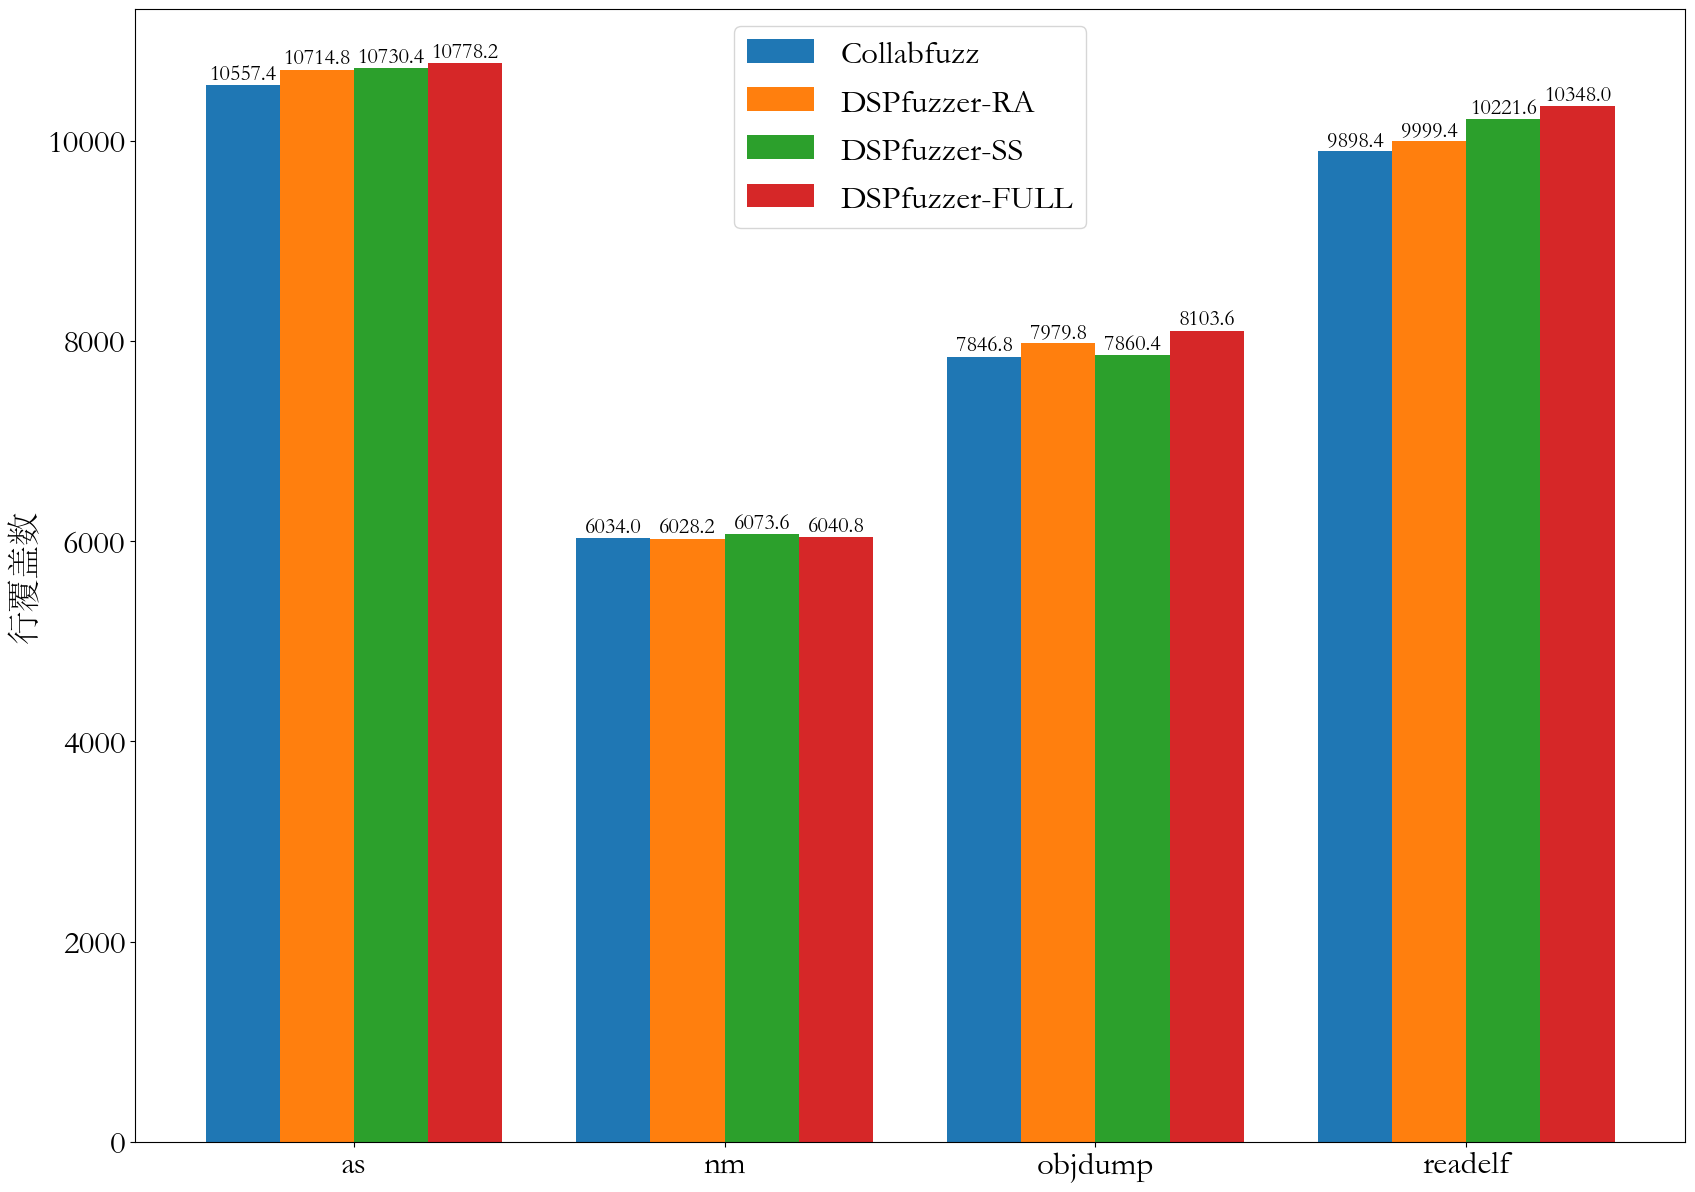
\includegraphics[width=13cm]{line.png}
    \caption{行覆盖指标测试结果}
    \label{line}
\end{figure}
 
行覆盖数的统计使用gcov工具进行插桩,需要在编译程序时添加“-fprofile-arcs”和“-ftest-coverage”选项。在实验结束后,按种子文件发现的时间顺序依次重新运行插桩后的程序,并在程序源码的主文件夹使用“gcovr -r . -s | grep "[l][a-z]*:"”命令收集具体的行覆盖信息。

通过实验可以得到四款被测试程序的行覆盖数,实验数据如图\ref{line}所示。对于被测试的四款软件,本系统的优化策略都比基准方法(Collabfuzz方法)的行覆盖数性能更优。三种优化策略相较基准方法,对被测软件的平均提升幅度为1.2\%、1.8\%和2.8\%。其中对as、objdump和readelf这三款软件的提升幅度相对较大,而对于nm,本系统的优化策略与基准测试接近,并没有观察到在行覆盖度量方面的显著提升。通过实验结果可以发现nm的行覆盖数明显少于其他三款软件,说明nm软件本身可覆盖的代码空间较小,因此能够提升的空间也十分有限。

(2)分支覆盖

分支覆盖数的统计同样使用gcov工具进行插桩,在编译程序时添加“-fprofile-arcs”和“-ftest-coverage”选项。在实验结束后,按种子文件发现的时间顺序依次重新运行插桩后的程序,并在程序源码的主文件夹使用“gcovr -r . -s | grep "[b][a-z]*:"”命令收集具体的行覆盖信息。

\begin{figure}[!htbp]
    \vspace{6pt}
    \centering
    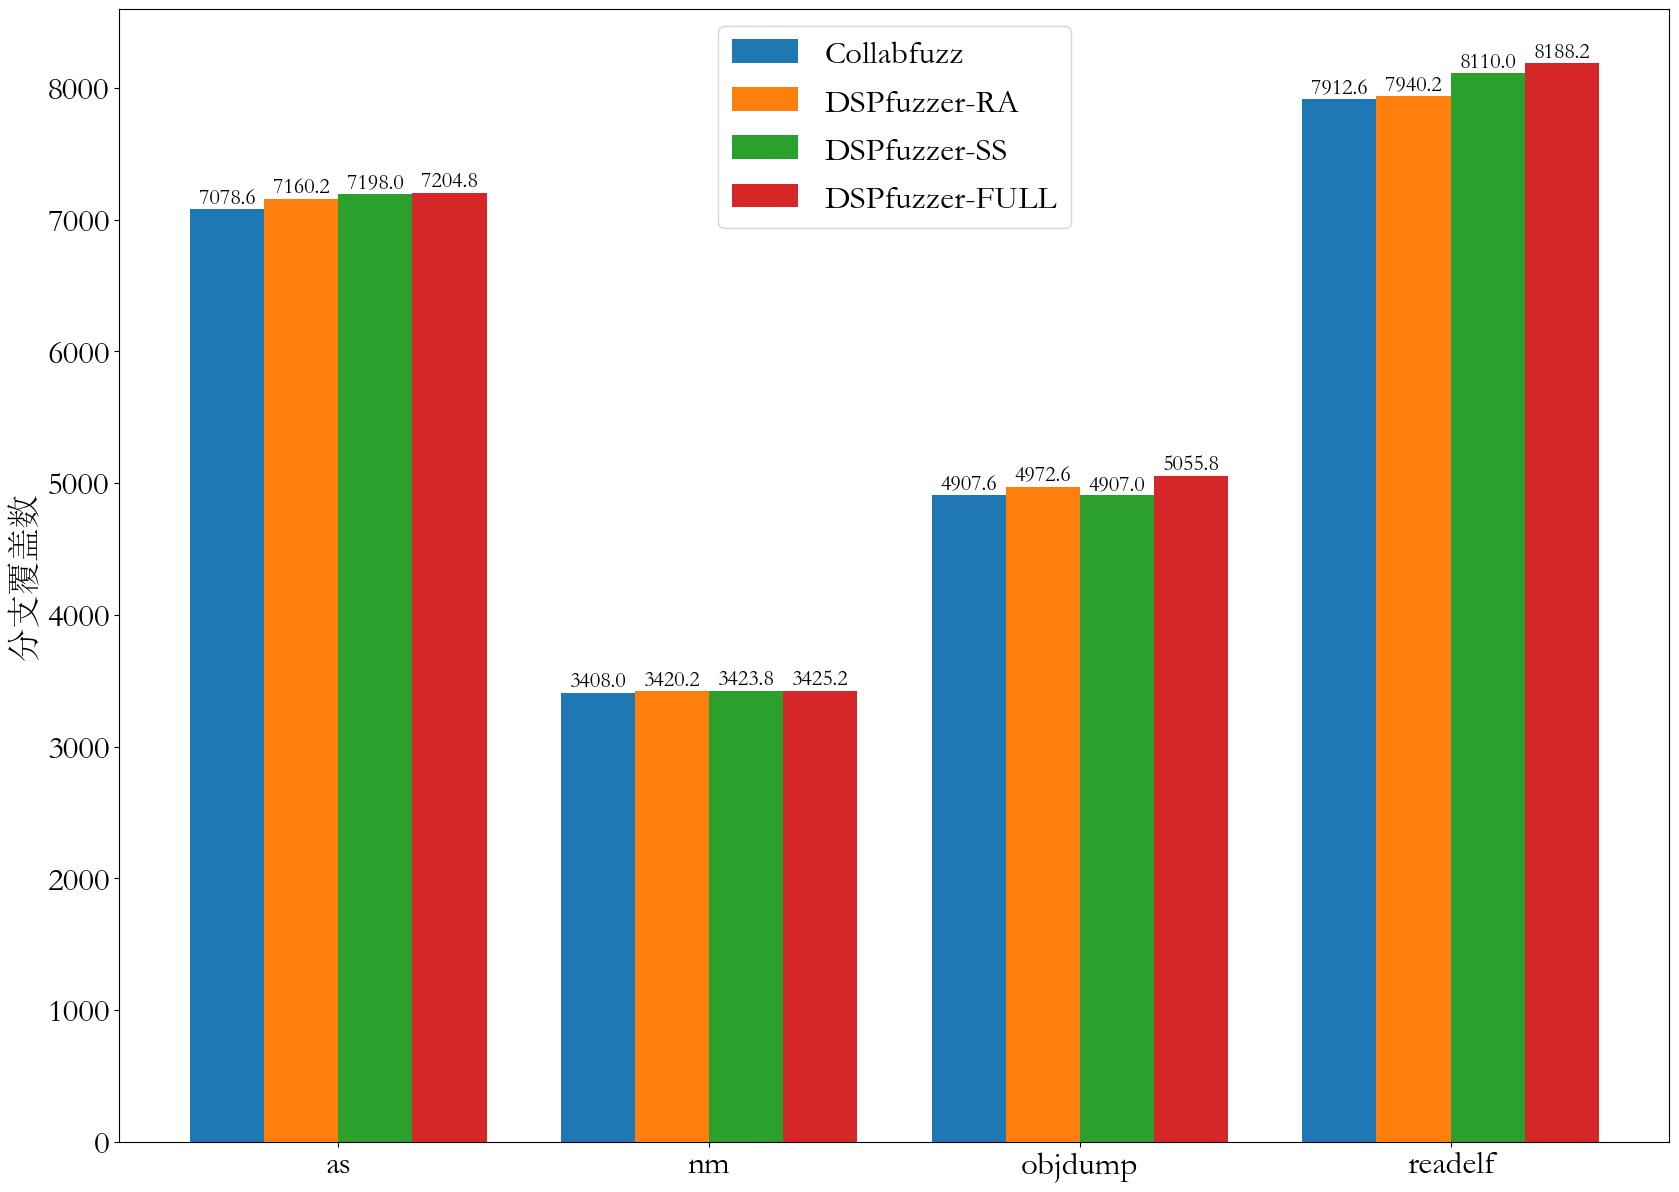
\includegraphics[width=13cm]{branch.png}
    \caption{分支覆盖指标测试结果}
    \label{branch}
\end{figure}

% AUC 指标显示覆盖率随时间的演变。在活动早期发现的覆盖范围越多,AUC 就越高。另一方面,稍后达到相同的结束覆盖将导致较低的 AUC 指标。为了使 AUC 指标更加具体,我们从中导出了一些样本。也就是说,查看实现部分覆盖范围的延迟是用户在使用有限的时间和资源进行模糊测试时可以预期的真实世界加速的有用指示。我们显示了达到总覆盖率的第 90、95、97 和 99 个百分位数的延迟差异。例如,如表 2 所示,EnFuzz 调度程序达到其末端覆盖率的 90\%,比成本效益快 13\%。

通过实验可以得到四款被测试程序的分支覆盖数,实验数据如图\ref{branch}所示。对于被测试的四款软件,本系统的优化策略都比基准方法(Collabfuzz方法)的分支覆盖数性能更优。三种优化策略相较基准方法,对被测软件的平均提升幅度为1.2\%、1.7\%和2.6\%。其中对as、objdump和readelf这三款软件的提升幅度相对较大,而对于nm,本系统的优化策略与基准测试接近,并没有观察到在行覆盖度量方面的显著提升。nm提升效果不明显的原因与行覆盖的结果相同。

(3)路径覆盖

路径覆盖数的统计使用AFL工具提供的分析方法,如果当前种子文件存在新执行的边信息,则认为发现了一条新的路径,路径覆盖数加一。

通过实验可以得到四款被测试程序的路径覆盖数,实验数据如图\ref{path_all}所示。对于被测试的四款软件,本系统的优化策略都比基准方法(Collabfuzz方法)的路径覆盖数性能更优。三种优化策略相较基准方法,对被测软件的平均提升幅度为4.5\%、4.7\%和6.9\%。其中对as、objdump和readelf这三款软件的提升幅度相对较大,而对于nm,本系统的优化策略与基准测试接近,并没有观察到在行覆盖度量方面的显著提升。nm提升效果不明显的原因与行覆盖的结果相同。可以发现,路径覆盖指标的提升高于行覆盖与分支覆盖,这是因为路径覆盖的粒度更细,更能反映出程序执行情况的多样性。

\begin{figure}[t]
    \vspace{6pt}
    \centering
    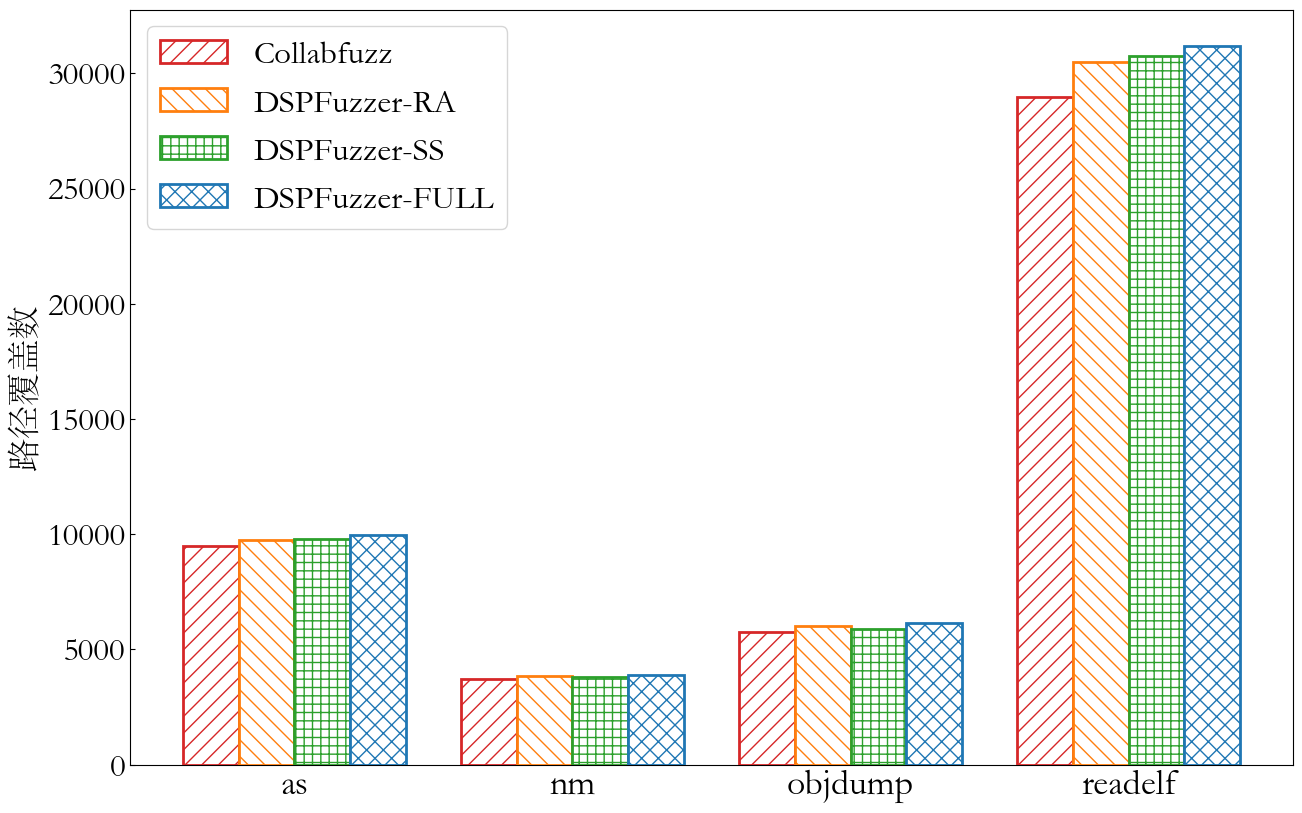
\includegraphics[width=15cm]{path_all.png}
    \caption{路径覆盖指标测试结果}
    \label{path_all}
\end{figure}

通过使用三种覆盖信息统计方式对测试结果进行评估,可以发现本系统的优化策略对测试大多数软件的代码覆盖信息有所提升,并且两种优化策略相结合能起到比单独实施一种策略更好的效果。对于测试覆盖结果提升不明显的软件nm,从三种覆盖统计数据可以发现明显少于其他三个软件,说明其可探索空间较小,因此本身能够提高的空间可能较为有限。


\subsection{崩溃数提升验证}

模糊测试中被测程序的崩溃数是另一个常用于评估模糊测试性能的指标,由于导致崩溃的原因可能相同,因此需要使用去重后的崩溃数作为指标,其中主流的去重方式有AFL使用的独特崩溃数统计方法和使用ASAN根据崩溃时的函数调用栈信息进行去重。

(1)独特崩溃数

其中独特崩溃数是AFL引入的指标,其统计逻辑与AFL的路径覆盖统计逻辑相同,如果当前崩溃的执行路径中存在之前崩溃情况中不曾存在的边信息时,认为这是一个独特的崩溃。可以在测试的过程中实时统计是它的一个较为明显的优点。

\begin{figure}[!htbp]
    \vspace{6pt}
    \centering
    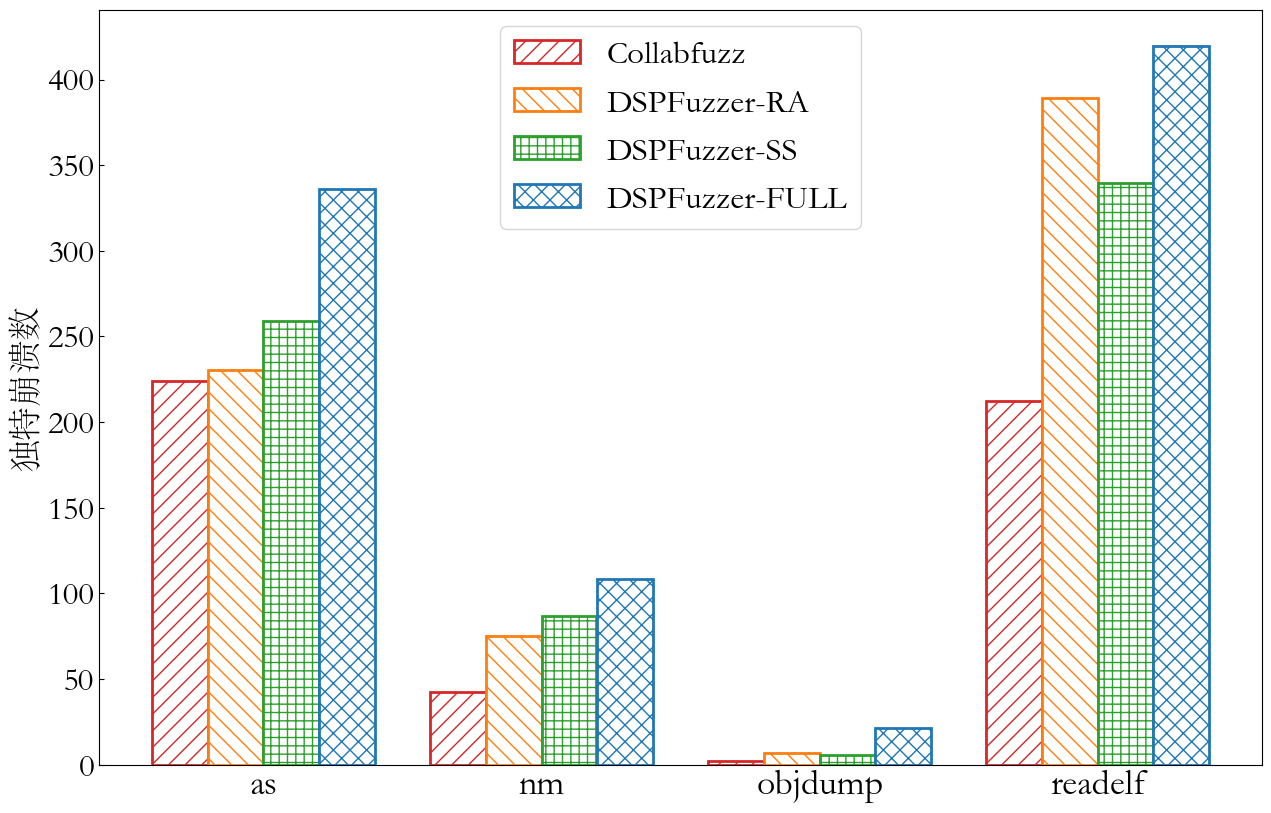
\includegraphics[width=14cm]{unique_bug.png}
    \caption{独特崩溃数指标测试结果}
    \label{unique_bug}
\end{figure}

通过实验可以得到四款被测试程序的独特崩溃数,实验数据如图\ref{unique_bug}所示。可以发现,独特崩溃数这项指标的统计结果波动较大,但是总体来说,本系统的优化策略比基准方法(Collabfuzz方法)的发现独特崩溃数更多。三种优化策略相较基准方法,对as、nm、objdump和readelf四款软件的平均提升幅度为46.1\%、43.8\%和84.5\%。

(2)ASAN去重崩溃数

内存消毒剂(Address Sanitizer,ASAN)也可以对崩溃情况进行去重,需要使用ASAN工具对源代码进行插桩,软件崩溃后会自动打印当前的函数调用栈,本次评估将对软件崩溃时最靠近栈顶的三个函数帧进行哈希,通过哈希值进行去重。

\begin{figure}[!htbp]
    \vspace{6pt}
    \centering
    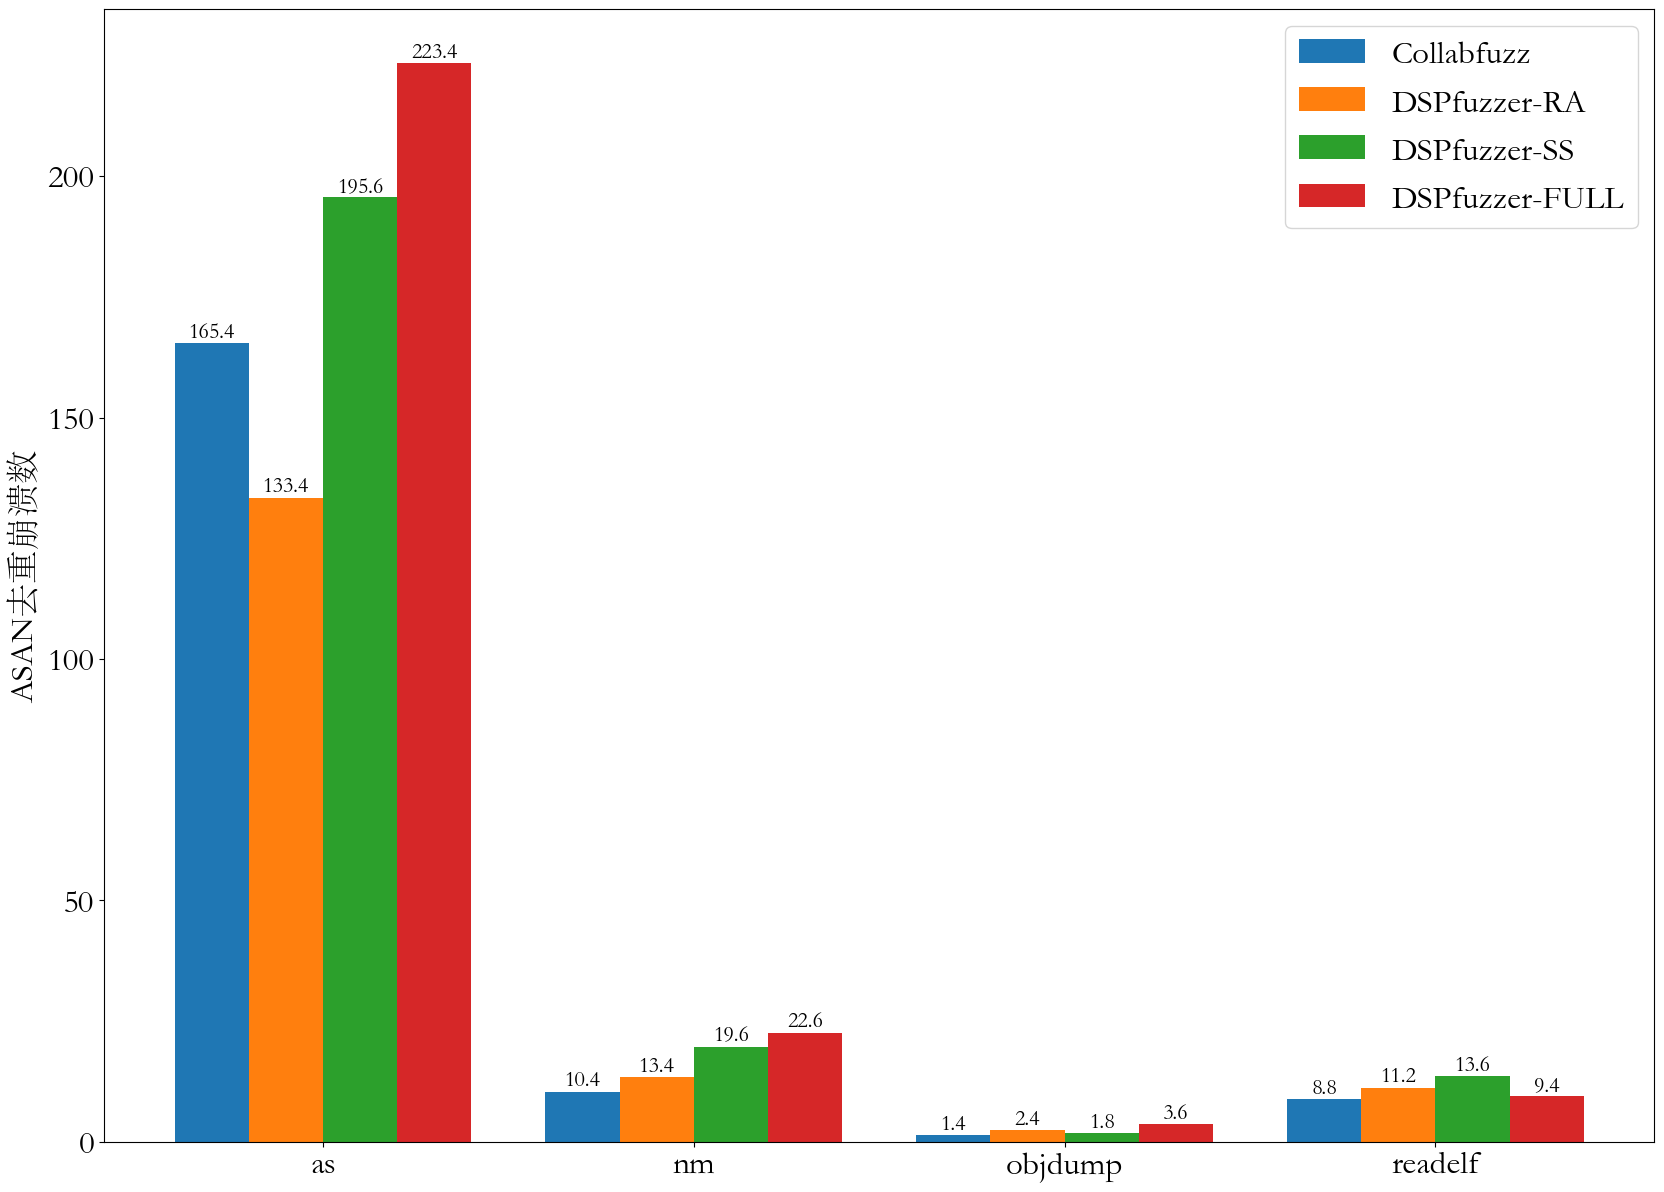
\includegraphics[width=14cm]{asan.png}
    \caption{ASAN去重崩溃数指标测试结果}
    \label{asan_bug}
\end{figure}

通过实验可以得到四款被测试程序ASAN去重后的崩溃数,实验数据如图\ref{unique_bug}所示。可以发现,ASAN去重后的崩溃数与独特崩溃数这一指标相比,它的绝对数值有了明显的下降,体现了良好的去重效果,消除了崩溃文件集的冗余。总体来说,本系统的优化策略比基准方法(Collabfuzz方法)发现的ASAN去重后崩溃数更多。三种优化策略相较基准方法,对as、nm、objdump和readelf四款软件的平均提升幅度为16.9\%、22.3\%和41.5\%。

通过使用两种崩溃数统计方式对测试结果进行评估,可以发现本系统的优化策略对测试大多数软件发现崩溃的能力有所提升,并且两种优化策略相结合能起到比单独实施一种策略更好的效果。

综上所述,本系统的优化策略在代码覆盖和崩溃数两个指标下,都有一定的提升效果,表明了动态策略并行模糊测试系统在测试性能上比已有工具有所提升。

\section{本章小结}

本章首先介绍了动态策略并行模糊测试系统验证实验的实验环境、选取的被测试软件和选取的模糊测试实例。接下来对测试系统细粒度信息收集能力进行验证,分析了收集数据的可用性。然后对测试系统的系统资源动态分配能了和跨实例种子调度能力进行验证,验证了系统功能的正确性。最后对测试系统测试效率提升能力进行验证,分别从代码覆盖率和崩溃数发现两个维度,对Binutils工具集下的四款软件(as、nm、objdump和readelf)进行测试与评估,结果表明动态策略并行模糊测试系统在12小时内,能够探索到更多的路径数、触发更多的崩溃数。 

\chapter{总结与展望}

\section{本文工作总结}

本文的核心工作是研究并实现动态策略并行模糊测试系统,系统相较于已有方法在测试效率上有所提升。主要研究成果和结论如下:

(1)给出了动态策略并行模糊测试系统整体框架。本文对当前并行模糊测试方案的优缺点进行分析,提出了动态策略并行模糊测试系统的设计目标,分别为收集细粒度信息、动态分配系统资源和跨实例调度种子,针对三大目标设计了动态策略并行模糊测试系统整体框架。

(2)给出了动态策略并行模糊测试系统关键技术。1)为了收集并行模糊测试中更多的测试数据,通过数据指导后续优化的实施,研究并实现信息收集与同步模块,能够对不同的模糊测试实例提取运行时的细粒度信息和同步种子文件。2)为了促进系统资源的高效利用,提高并行模糊测试整体的测试效率,研究并实现了系统资源动态分配模块。该模块能够根据并行模糊测试的历史执行情况有效预测未来时间段各模糊测试实例的效率,并根据预测结果对各模糊测试实例占用的系统资源进行调整,使得效率高的模糊测试实例能够执行更多的模糊测试。3)为了减少并行模糊测试中的测试冗余,提高并行模糊测试整体的测试效率,分析并得到种子效率与种子执行次数成负相关的关系,实现了跨实例种子调度模块,通过全局数据库使得模糊测试实例能够减少高执行次数种子的选择概率。

(3)开展了动态策略并行模糊测试系统验证实验。首先,以nm软件的测试过程为例,展示了并行模糊测试中能够获取并利用的信息。然后对测试系统的系统资源动态分配能了和跨实例种子调度能力进行验证,验证了系统功能的正确性。最后,将系统对Binutils工具集中as、nm、objdump和readelf四款软件的测试结果进行分析,并将测试结果与Collabfuzz的测试结果进行对比:1)对于代码覆盖率提升的验证,在行覆盖、分支覆盖和路径覆盖上分别提升2.8\%、2.6\%和6.9\%;2)对于崩溃数的验证,在独特崩溃数和ASAN去重后崩溃数上分别提升84.5\%、41.5\%,结果表明,本文设计的动态资源并行模糊测试系统能够有效提取测试中的细粒度信息,并提高并行模糊测试整体的测试效率。

\section{后续研究方向}

本文主要从收集细粒度信息、提高测试效率两个方面对并行模糊测试技术进行探讨,未来的研究可以从以下方面开展:1)在本文设计的并行模糊测试系统中,模糊测试实例在测试前已选择并不能更改,由于模糊测试工具提升测试能力的方向和技术的不同,不一定能够选择出最佳的测试组合,因此可以在测试过程中动态挑选并更改运行的模糊测试实例组合,以达到最佳的测试效果。2)同构并行模糊测试相较于异构并行模糊测试有测试冗余小的优势,因此可以在同构并行模糊测试的框架下,研究不同模糊测试技术的综合应用方式。

\thesisacknowledgement

光阴似箭,日月如梭,转眼间我即将完成我的硕士研究生学业。在这段求学的岁月里,我收获了太多太多。

首先,我要向我的导师孙罡教授表达我最诚挚的感激之情。在我的硕士研究生期间,他一直给予我细致入微的指导和耐心的教诲,不仅在学术研究方面为我提供了宝贵的建议和指导,更为我树立了良好的人生导向。在这条研究之路上,他的教诲成为了我前行的指路明灯,他的谆谆教诲也将会伴随我今后的一生。

其次,我要感谢我的家人。是他们默默地支持我,承受着我离家在外的寂寞,他们的爱与支持给我带来了无限的力量。他们不仅在物质上给予我支持,还鼓励我,支持我,在研究的起伏中始终给我信心,给我支持和帮助,让我在求学的道路上有了更坚实的基础和更好的信念。

同时,我也要感谢我的同学和朋友们。在这段学习的岁月里,我得到了很多同学的支持和帮助,他们共同分享了我在这个学术领域的经验,一起讨论,一起进步。在我遇到困难时,他们始终给予我鼓励和支持,让我更有信心和勇气面对学术挑战。

最后,我要向所有在这段学习中给予我支持和帮助的人们表示最真诚的感谢。没有你们的鼓励、支持和帮助,我无法走到今天的成果,你们是我不断前行的动力和勇气。感谢你们在这段学习中的陪伴和支持,我将永远铭记于心。

\thesisbibliography{reference} % 参考文献

\titlespacing{\section}{-24pt}{18pt}{6pt}
\begin{thesistheaccomplish}
	
	
	\section*{发表论文:}
	\bibitem[1]{} 王晓楠,\textbf{符劲轩},虞红芳,孙罡,陈海兵.基于抽象原则和模型检测的网络协议安全分析[J].北京邮电大学学报,2021,44(02):40-46.
	\bibitem[2]{} Li S, Li J, \textbf{Fu J}, et al. Protocol Fuzzing With Specification Guided Message Generation[C]. 2021 International Conference on UK-China Emerging Technologies (UCET). IEEE, 2021: 164-170.

	
	\section*{参与项目:}
	\bibitem[1]{} 中国电子科技集团公司第三十研究所合作项目“协议建模与代码分析软件”,项目编号:200237,2019年9月—2020年12月.
	
\end{thesistheaccomplish}
\titlespacing{\section}{0pt}{18pt}{6pt}

% \begin{thesistheaccomplish}
%     \section{发表论文:}
%     \bibitem{SGXDedup} 王晓楠,\textbf{符劲轩},虞红芳,孙罡,陈海兵.基于抽象原则和模型检测的网络协议安全分析[J].北京邮电大学学报,2021,44(02):40-46.
%     \bibitem{SGXDedup} Li S, Li J, \textbf{Fu J}, et al. Protocol Fuzzing With Specification Guided Message Generation[C]. 2021 International Conference on UK-China Emerging Technologies (UCET). IEEE, 2021: 164-170.
%     \section{参与项目:}
%     \bibitem{CN111338572B} 中国电子科技集团公司第三十研究所合作项目“协议建模与代码分析软件”,项目编号:200237,2019年9月—2020年12月.
% \end{thesistheaccomplish}

\end{document}
